%% LaTeX2e class for student theses
%% sections/apendix.tex
%% 
%% Karlsruhe Institute of Technology
%% Institute for Program Structures and Data Organization
%% Chair for Software Design and Quality (SDQ)
%%
%% Dr.-Ing. Erik Burger
%% burger@kit.edu
%%
%% Version 1.3.6, 2022-09-28

\iflanguage{english}
{\chapter{Appendix}}    % english style
{\chapter{Anhang}}      % german style
\label{chap:appendix}


%% -------------------
%% | Example content |
%% -------------------
\section{Proof of Data points trained using Active Learning}
\label{sec:appendix:FirstSection}
\begin{theorem}
Let $X$ be a set of data points of size $n$, $b < n, n \mod b = 0$ be the batch size. Then a machine learning model trained
using pool-based Active Learning is trained $\frac{n}{b}$ times on the current labeled pool of data points. Overall, the model
is trained on $\frac{n(n+b)}{2b}$ data points
\end{theorem}
\begin{proof}
    The first part is trivial, given that the model is trained until the labeled pool is exhausted and in each iteration $b$
    points are queried for their label. To determine the total number of points used, we need to sum up the number of points
    used in each iteration. 
    \begin{equation}
        \sum_{i=1}^{\frac{n}{b}} i \cdot b
    \end{equation}
    Using the formula for the sum of the first $n$ natural numbers, we get
    \begin{equation}
        \sum_{i=1}^{\frac{n}{b}} i \cdot b = b \cdot \sum_{i=1}^{\frac{n}{b}} i = b \cdot \frac{\frac{n}{b} (\frac{n}{b} + 1)}{2}
        = \frac{n (\frac{n}{b} + 1)}{2} = \frac{n(n+b)}{2b}
    \end{equation}
\end{proof}

\section{Specifications}
\label{sec:Appendix:Specifications}
In this section, we will list tables containing the specifications of the hardware and software used in our experiments.

\begin{table}[h!]
    \begin{tabularx}{\textwidth}{|X | X X X|} 
        \hline
         & GPU x4 & GPU x8 & GPU x4 A100 \\ 
        \hline 
        Processors & Intel Xeon Gold 6230 & Intel Xeon Gold 6248 & Intel Xeon Platinum 8358  \\ 
        Number of sockets & 2 & 2 & 2  \\ 
        Processor frequency (GHz) & 2.1 & 2.6 & 2.5  \\ 
        Total number of cores & 40 & 40 & 64  \\ 
        Main memory & 384 GB & 768 GB & 512 GB  \\ 
        Local SSD & 3.2 TB NVMe & 15TB NVMe & 6.4 TB NVMe  \\ 
        GPUs & 4x NVIDIA Tesla V100 & 8x NVIDIA Tesla V100 & 4x NVIDIA A100  \\ 
        GPU Memory & 32 GB  & 32 GB & 80 GB  \\ 
        Interconnect & IB HDR & IB HDR & IB HDR200  \\ 
        \hline
    \end{tabularx}
    \caption{Hardware configuration for the three nodes used on BWUniCluster. This table only contains
    the nodes we used in our experiments. For a more detailed list of all nodes as well as all further
    information, see \cite{bwUniclusterHardware}}
    \label{fig:HardwareSpec}
\end{table}

\begin{table}[h!]
    \centering
    \begin{tabular}{|l | l l |} 
        \hline
        Library Name & Version & Link \\ 
        \hline 
        numpy & 1.23.0 & \url{https://numpy.org/} \\
        tqdm & 4.64.1 & \url{https://tqdm.github.io/}  \\
        torchvision & 0.14.1 & \url{https://pytorch.org/vision/stable/index.html} \\ 
        torch & 1.13.1 & \url{https://pytorch.org/} \\
        PyYAML & 6.0 & \url{https://pyyaml.org/} \\
        scipy & 1.10.1 & \url{https://scipy.org/} \\
        scikit-learn & 1.2.1 & \url{https://scikit-learn.org/stable/index.html} \\
        wget & 3.2 & \url{https://pypi.org/project/wget/} \\
        \hline
    \end{tabular}
    \caption{Software Libraries used for the experiments}
    \label{fig:Libraries}
\end{table}

\begin{table}[h!]
    \begin{tabularx}{\textwidth}{|l | X | l |} 
        \hline
        Hyperparameter & Description & Value \\ 
        \hline 
        $\lambda$ & Balances between old and new tasks. A higher value \newline indicates more focus 
        on preserving knowledge from \newline the old task & 1.0  \\ 
        Sample size & Relative size of the sample compared to the \newline full training set that is used to 
        compute \newline the Fisher Matrix & 0.05  \\ 
        Gradient Clip & Maximum Value of the $l2$-Norm of the gradient. \newline If the current norm is larger, the \newline
        gradient is clipped to that value & 20.0 \\ 
        \hline
    \end{tabularx}
    \caption{Hyperparameter configuration for \gls{ewc}.}
    \label{fig:EWCparams}
\end{table}

\begin{table}[h!]
    \begin{tabularx}{\textwidth}{| l | X | l |} 
        \hline
        Hyperparameter & Description & Value \\ 
        \hline 
        $\lambda$ & Balances between old and new tasks. A higher value indicates \newline more focus
        on preserving knowledge \newline from the old task & 1.0  \\ 
        Gradient Clip & Maximum Value of the $l2$-Norm of the gradient. If \newline the current norm is larger, the
        gradient \newline is clipped to that value & 2.0 \\ 
        \hline
    \end{tabularx}
    \caption{Hyperparameter configuration for \gls{mas}.}
    \label{fig:MASparams}
\end{table}

\begin{table}[h!]
    \begin{tabularx}{\textwidth}{| l | X | l |} 
        \hline
        Hyperparameter & Description & Value \\ 
        \hline 
        $\lambda$ & Balances between old and new tasks. A higher value indicates \newline more focus
        on preserving knowledge \newline from the old task & 1.0  \\ 
        Gradient Clip & Maximum Value of the $l2$-Norm of the gradient. If \newline the current norm is larger, the
        gradient is clipped to that value & 20.0 \\ 
        $\alpha$ & Weights the importance of the previous tasks. The sum of all $\alpha$ values must be 1.0 & 0.45,0.55 \\
        \hline
    \end{tabularx}
    \caption{Hyperparameter configuration for \gls{imm}.}
    \label{fig:IMMparams}
\end{table}

\begin{table}[h!]
    \centering
    \begin{tabularx}{\textwidth}{| l | X | l |} 
        \hline
        Hyperparameter & Description & Value \\ 
        \hline 
        $a$ & Balances between old and new tasks. A higher value indicates \newline more focus
        on preserving knowledge from the old task & 0.5  \\ 
        $a'$ & Used to update parameter importances in Equation TODO & 0.25  \\
        Gradient Clip & Maximum Value of the $l2$-Norm of the gradient. If \newline the current norm is larger, the
        gradient is clipped to that value & 2.0 \\ 
        $c$ & Determines the overestimation of the loss on the unobserved side & 3.0 \\
        $c'$ & Used to update parameter importances in Equation TODO & 1.5 \\
        \hline
    \end{tabularx}
    \caption{Hyperparameter configuration for \gls{alasso}.}
    \label{fig:AlassoParams}
\end{table}


\begin{table}[h!]
    \centering
    \begin{tabularx}{\textwidth}{|X | X X X X|} 
        \hline
         & MNIST & CIFAR-10 & Tiny \newline ImageNet & Small \newline ImageNet \\ 
        \hline 
        Size of training set & 60000 & 50000 & 100000 & 128116 \\ 
        Size of validation set & 10000 & 10000 & 10000 & 50000\\
        Number of classes & 10 & 10 & 200 & 1000 \\
        Image Dimension & 28x28 & 32x32 & 64x64& 32x32\\
        Number of channels & 1 & 3 & 3 & 3 \\
        Source & torchvision & torchvision & {\small \url{http://cs231n.stanford.edu/tiny-imagenet-200.zip}} & {\small \url{http://www.image-net.org/data/downsample/Imagenet32_32.zip}} \\
        \hline
    \end{tabularx}
    \caption{Information on the datasets used for the experiments.}
    \label{fig:DatasetInformtion}
\end{table}

\begin{figure}[h]
    \centering
    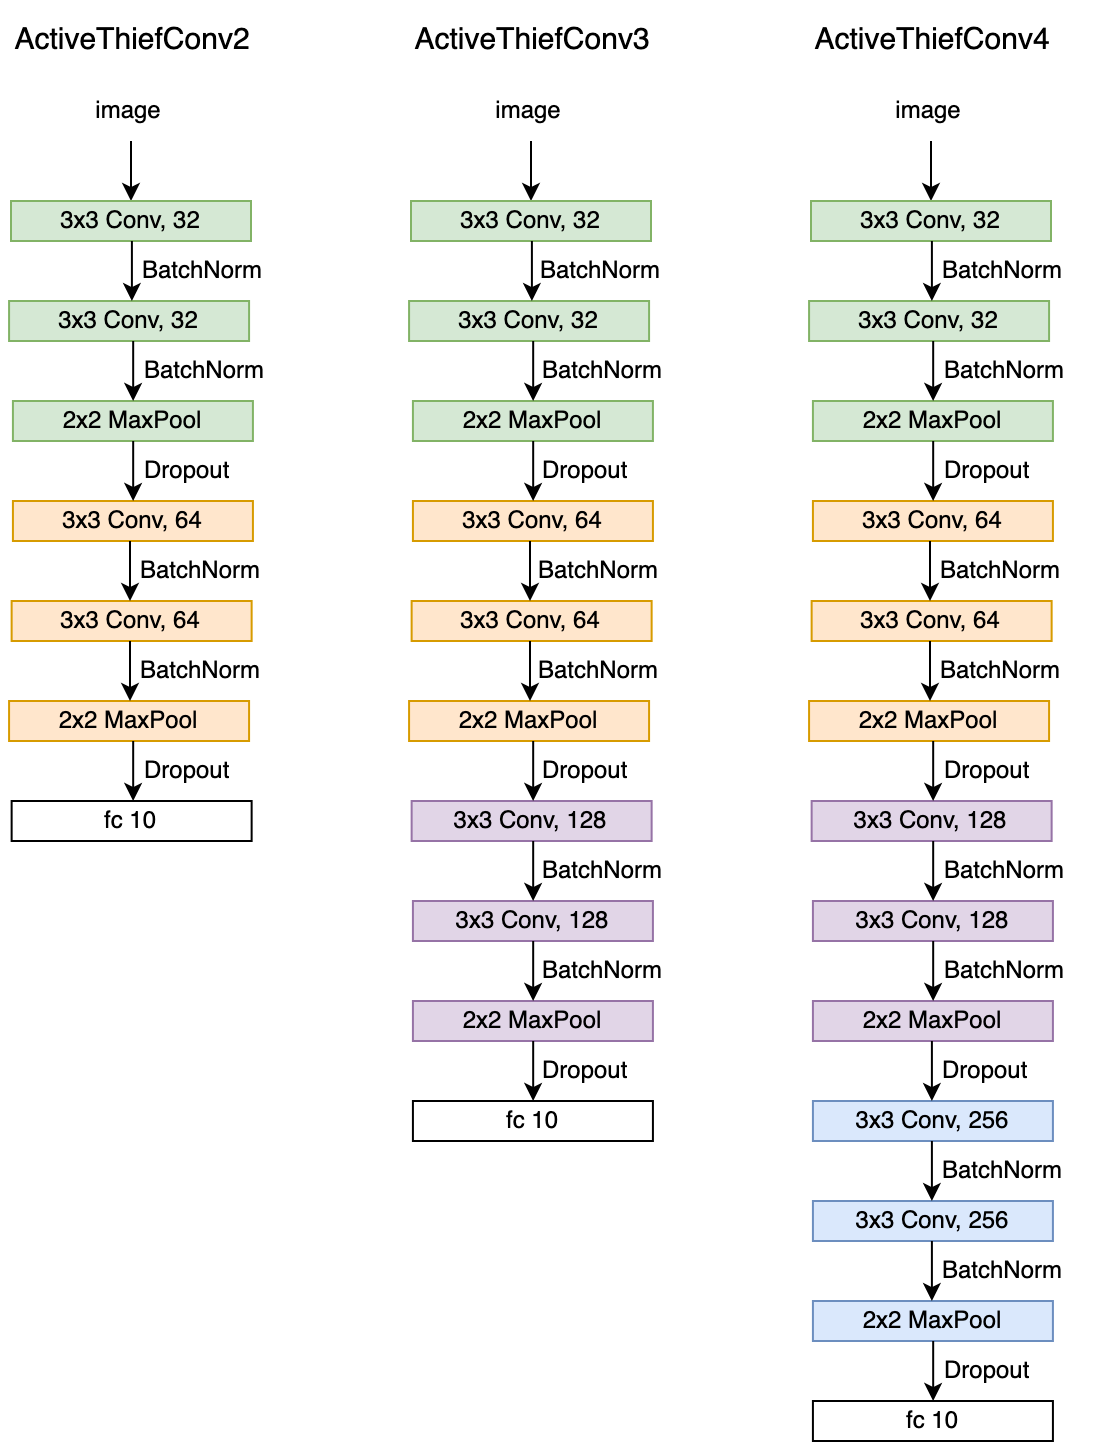
\includegraphics[width=\linewidth]{images/ActiveThiefConvs.png}
    \caption[ActiveThiefConv Architectures]{Example Network Architectures for CIFAR-10.}
    \label{fig:ActiveThiefArchitectures}
\end{figure}



\section{Experimental Results}
\label{sec:Appendix:Results}

\begin{figure}[h]
    \centering
    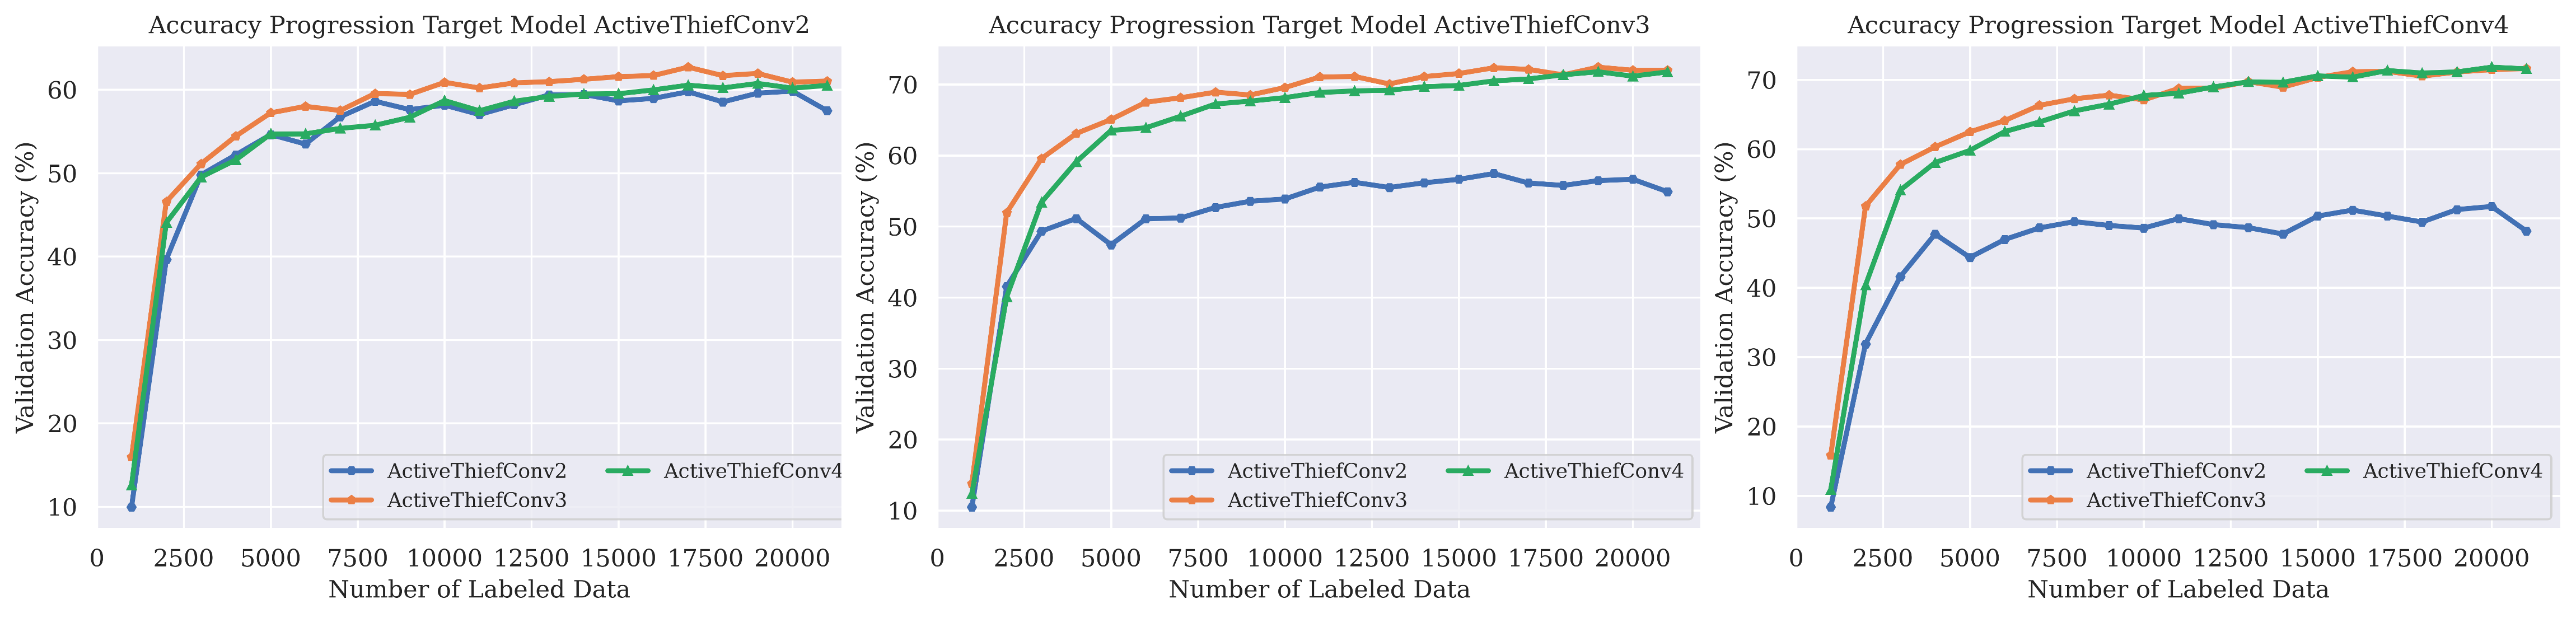
\includegraphics[width=\linewidth]{images/results_CALMS/cifar10_model_comp.png}
    \caption[Agreement Progression for Model Stealing on CIFAR-10 using different ActiveThief models]{Progression of Model
    Agreement (in \%) for Model Stealing Attacks using Active Learning on the CIFAR-10 dataset. We compare the Target and Substitute Model architectures
    ActiveThiefConv2, ActiveThiefConv3 and ActiveThiefConv4.}
    \label{fig:CIFAR10modelComp}
\end{figure}

\begin{figure}[h]
    \centering
    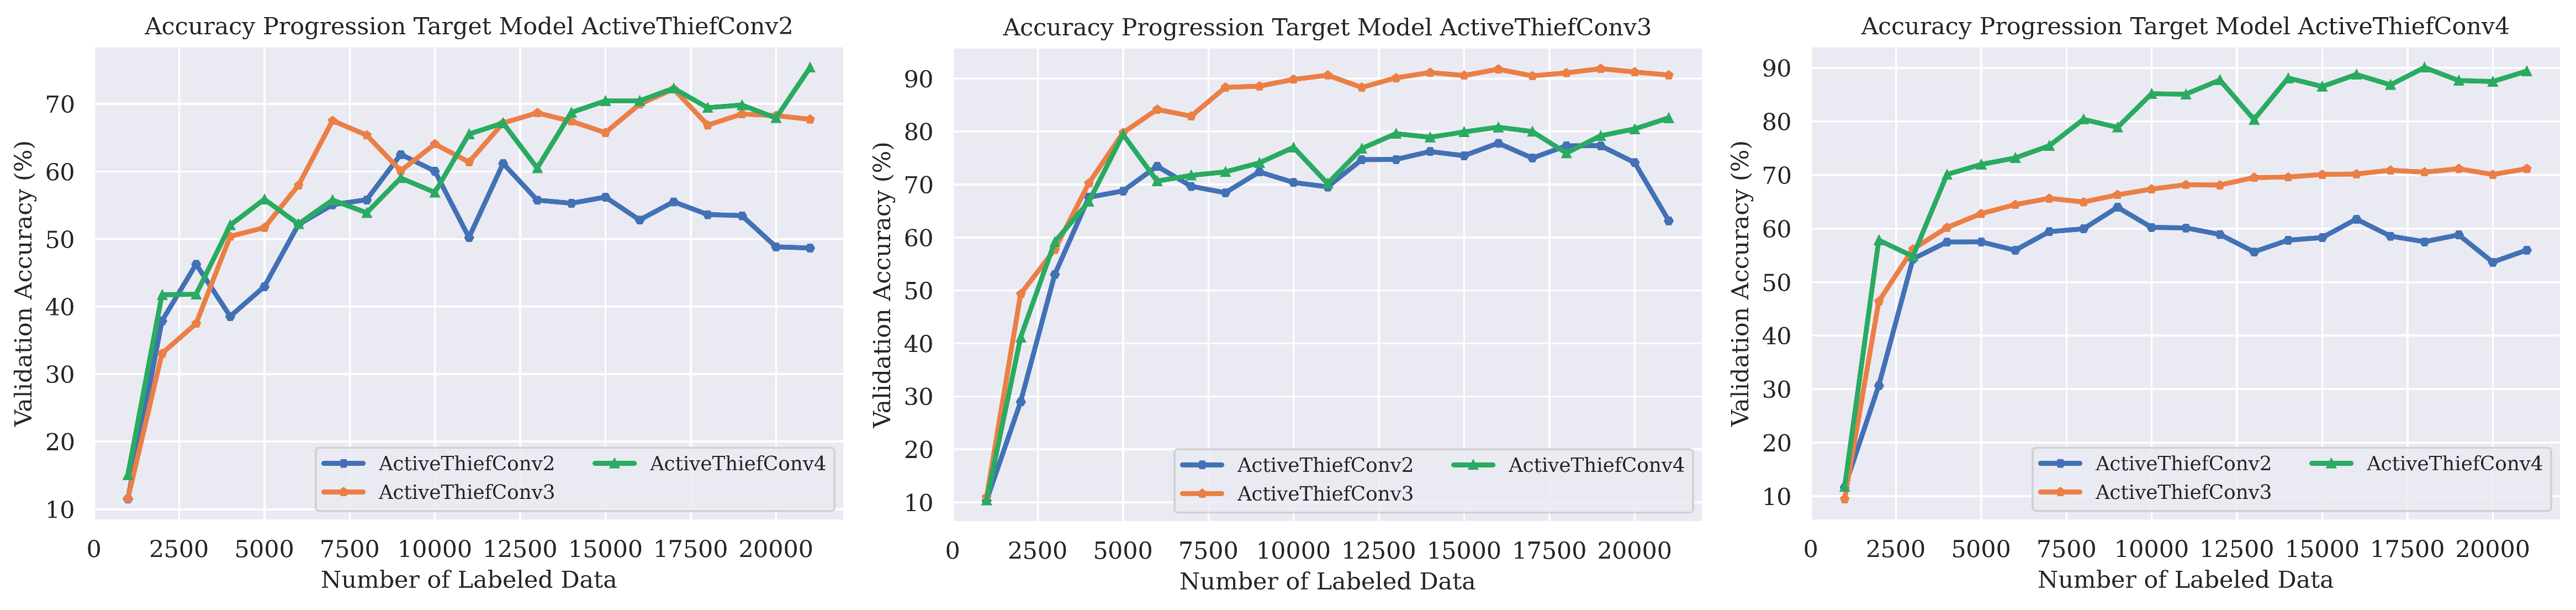
\includegraphics[width=\linewidth]{images/results_CALMS/mnist_model_comp.png}
    \caption[Agreement Progression for Model Stealing on MNIST using different ActiveThief models]{Progression of Model
    Agreement (in \%) for Model Stealing Attacks using Active Learning on the MNIST dataset. We compare the Target and Substitute Model architectures
    ActiveThiefConv2, ActiveThiefConv3 and ActiveThiefConv4.}
    \label{fig:MNISTmodelComp}
\end{figure}


%Tables for Cifar100
\begin{figure}[h]
    \centering
    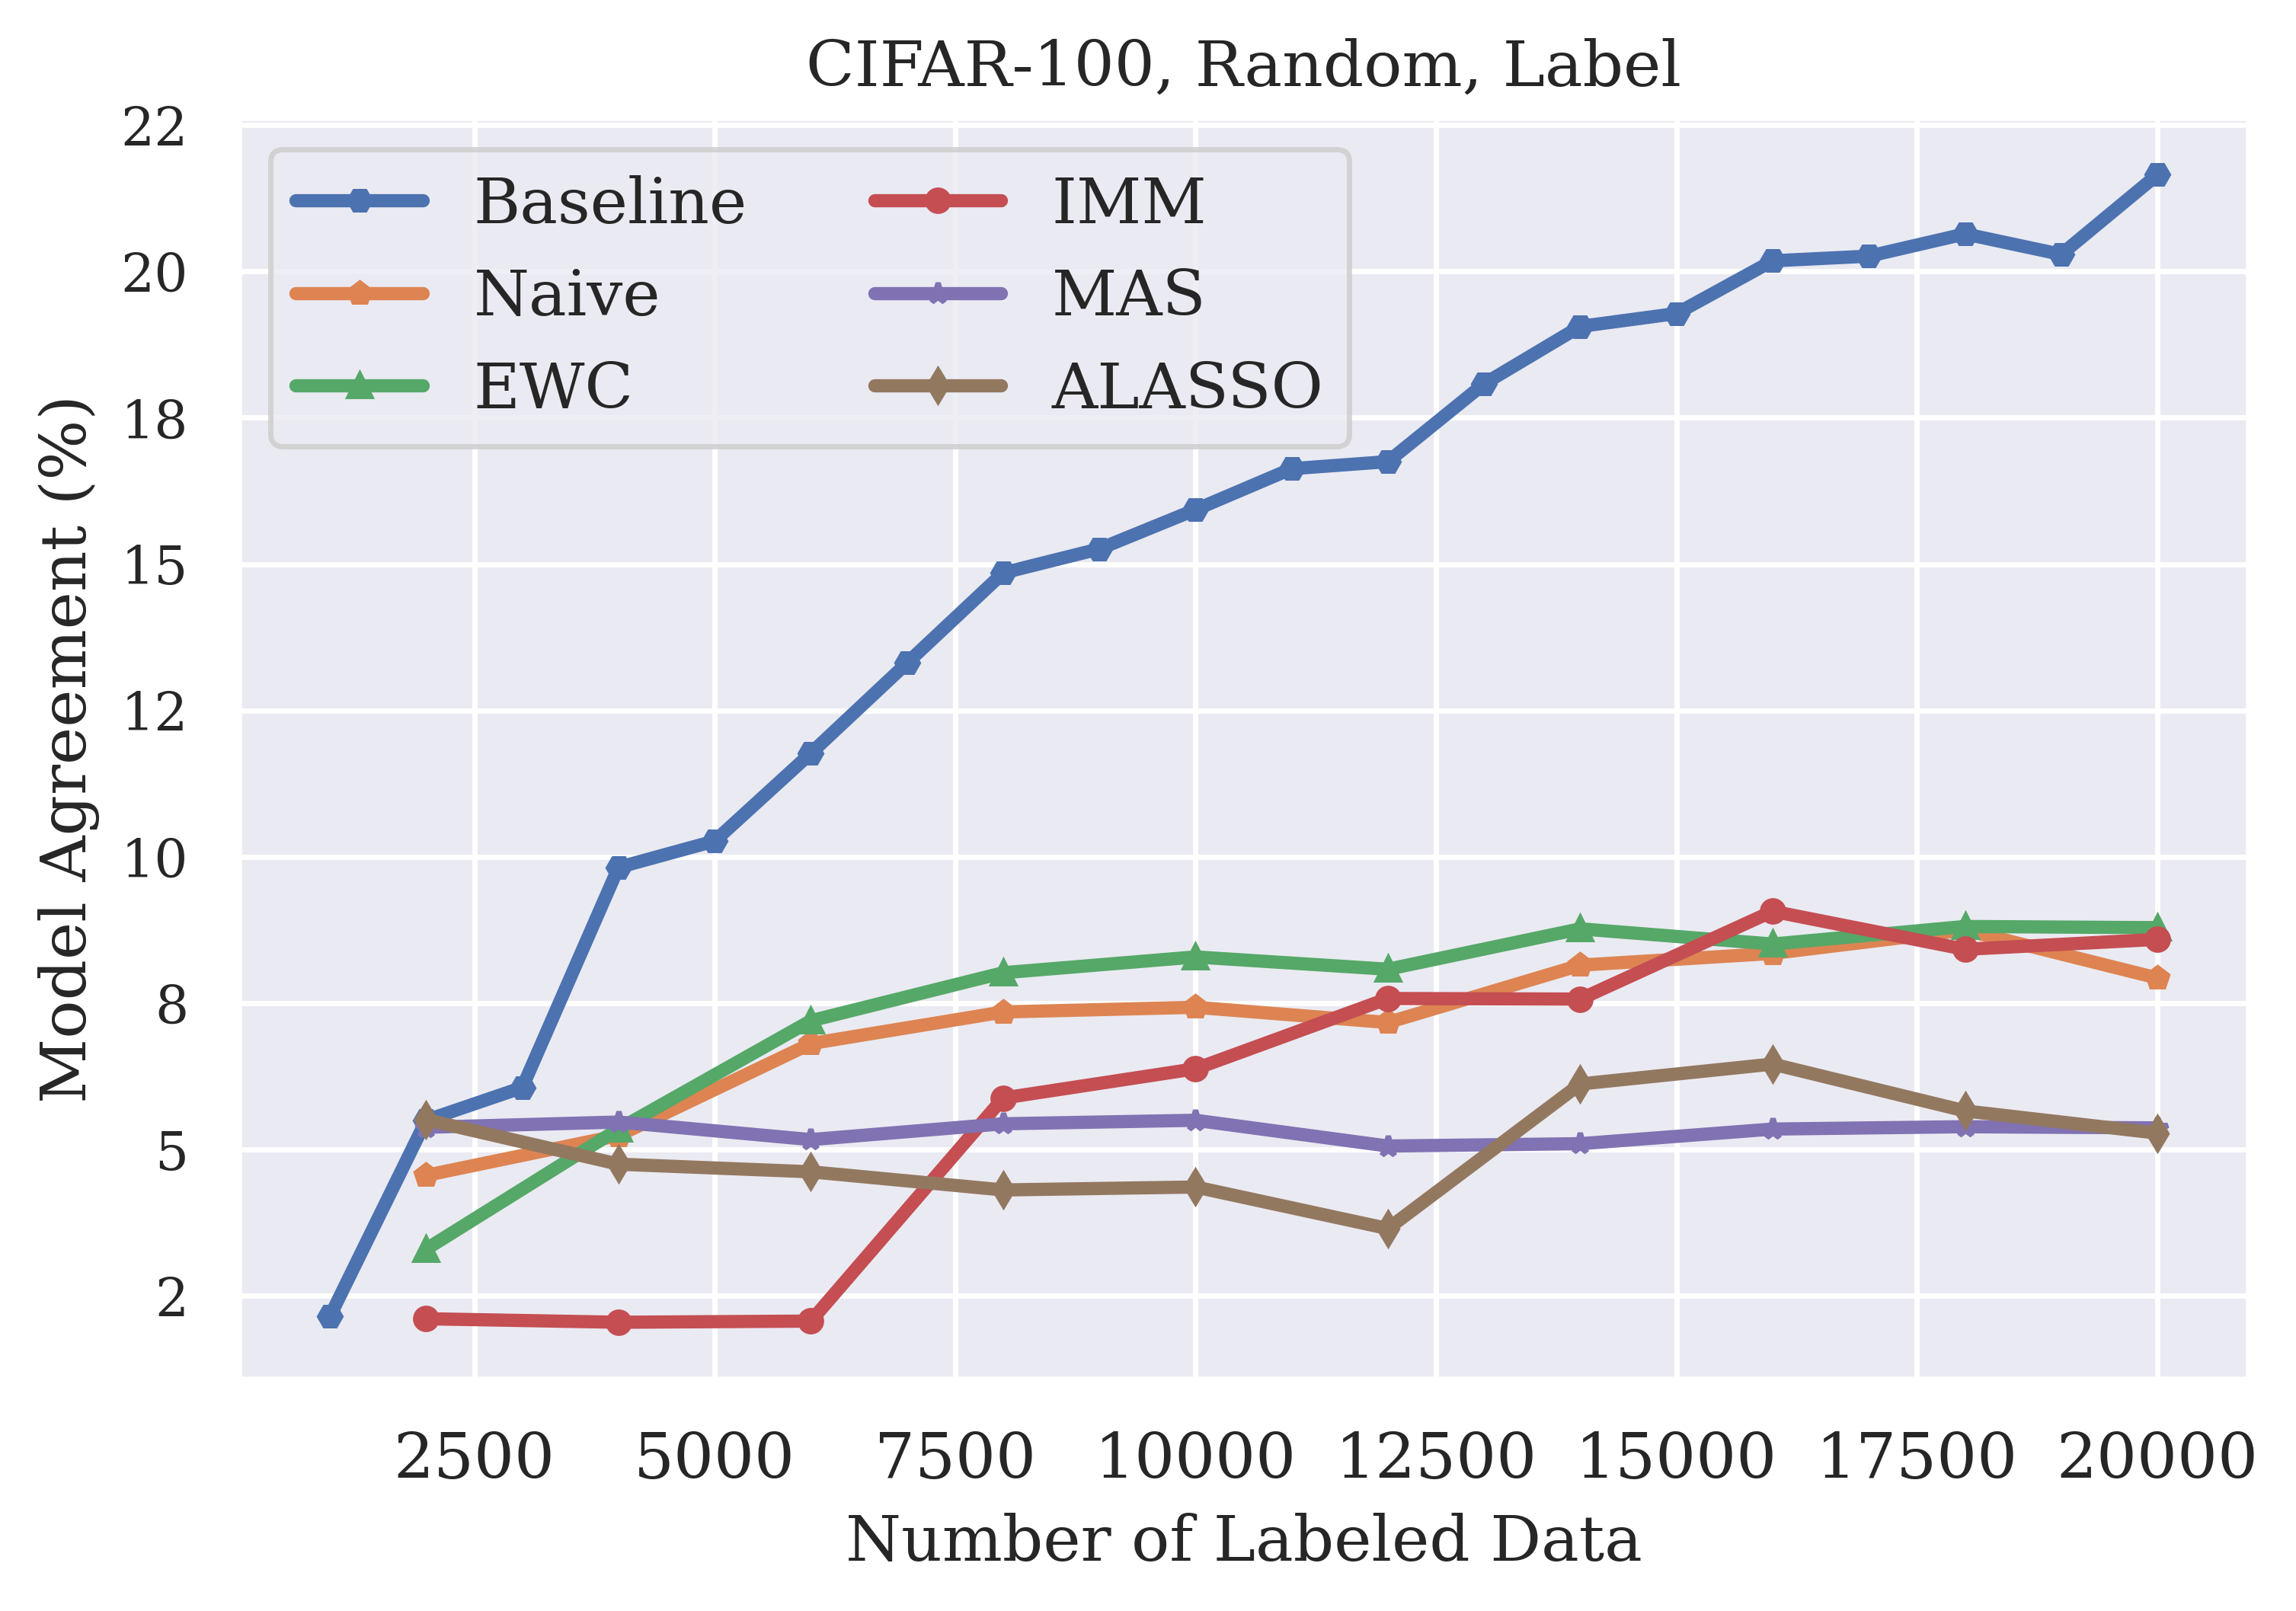
\includegraphics[width=0.7\linewidth]{images/results_CALMS/cifar100_label_random.png}
    \caption[Agreement Comparison for Model Stealing on CIFAR100 using the predicted class label and the Active Learning strategy Random]{Progression of Model
    Agreement (in \%) for Model Stealing Attacks using Continual Active Learning on the CIFAR-100 dataset. We use Model Stealing Attacks with random sampling
    and train using the predicted class label of the Target Model.}
    \label{fig:CALMSCIFAR100LabelRandom}
\end{figure}

\begin{figure}[h]
    \centering
    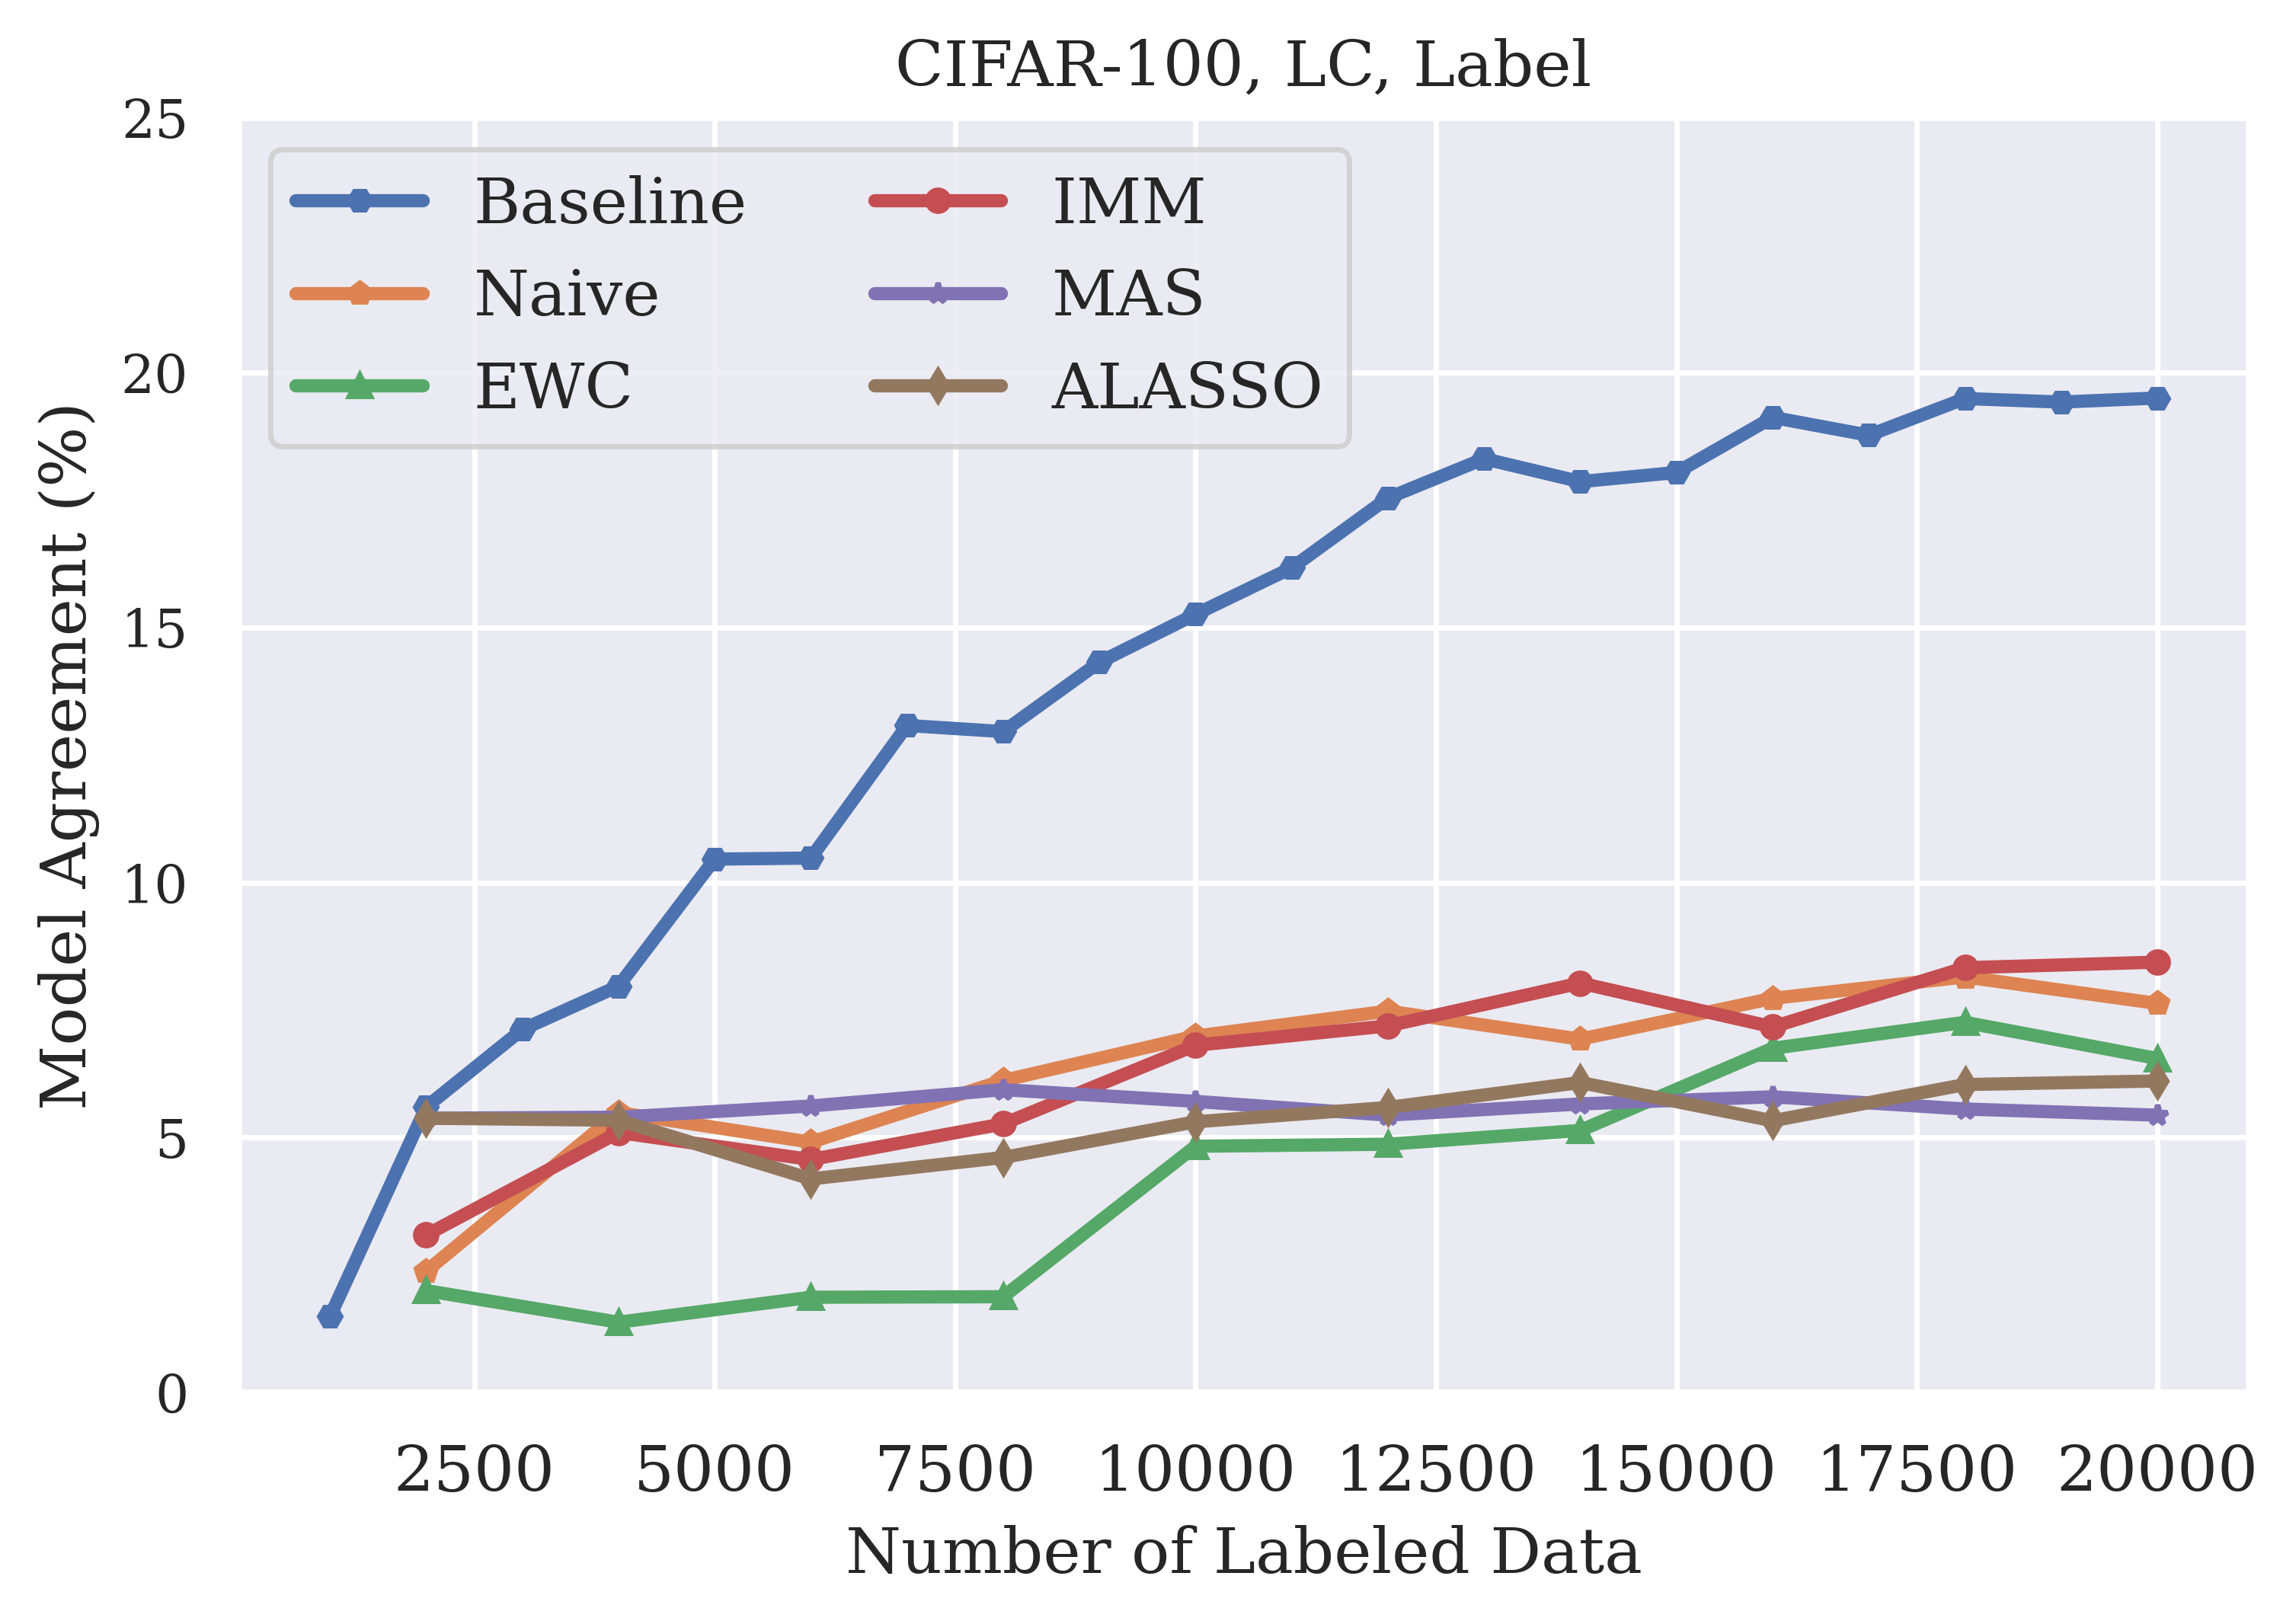
\includegraphics[width=0.7\linewidth]{images/results_CALMS/cifar100_label_lc.png}
    \caption[Agreement Comparison for Model Stealing on CIFAR100 using the predicted class label and the Active Learning strategy LC]{Progression of Model
    Agreement (in \%) for Model Stealing Attacks using Continual Active Learning on the CIFAR-100 dataset. We use Model Stealing Attacks with the Active Learning
    strategy \gls{lc} and train using the predicted class label of the Target Model.}
    \label{fig:CALMSCIFAR100LabelLC}
\end{figure}

\begin{figure}[h]
    \centering
    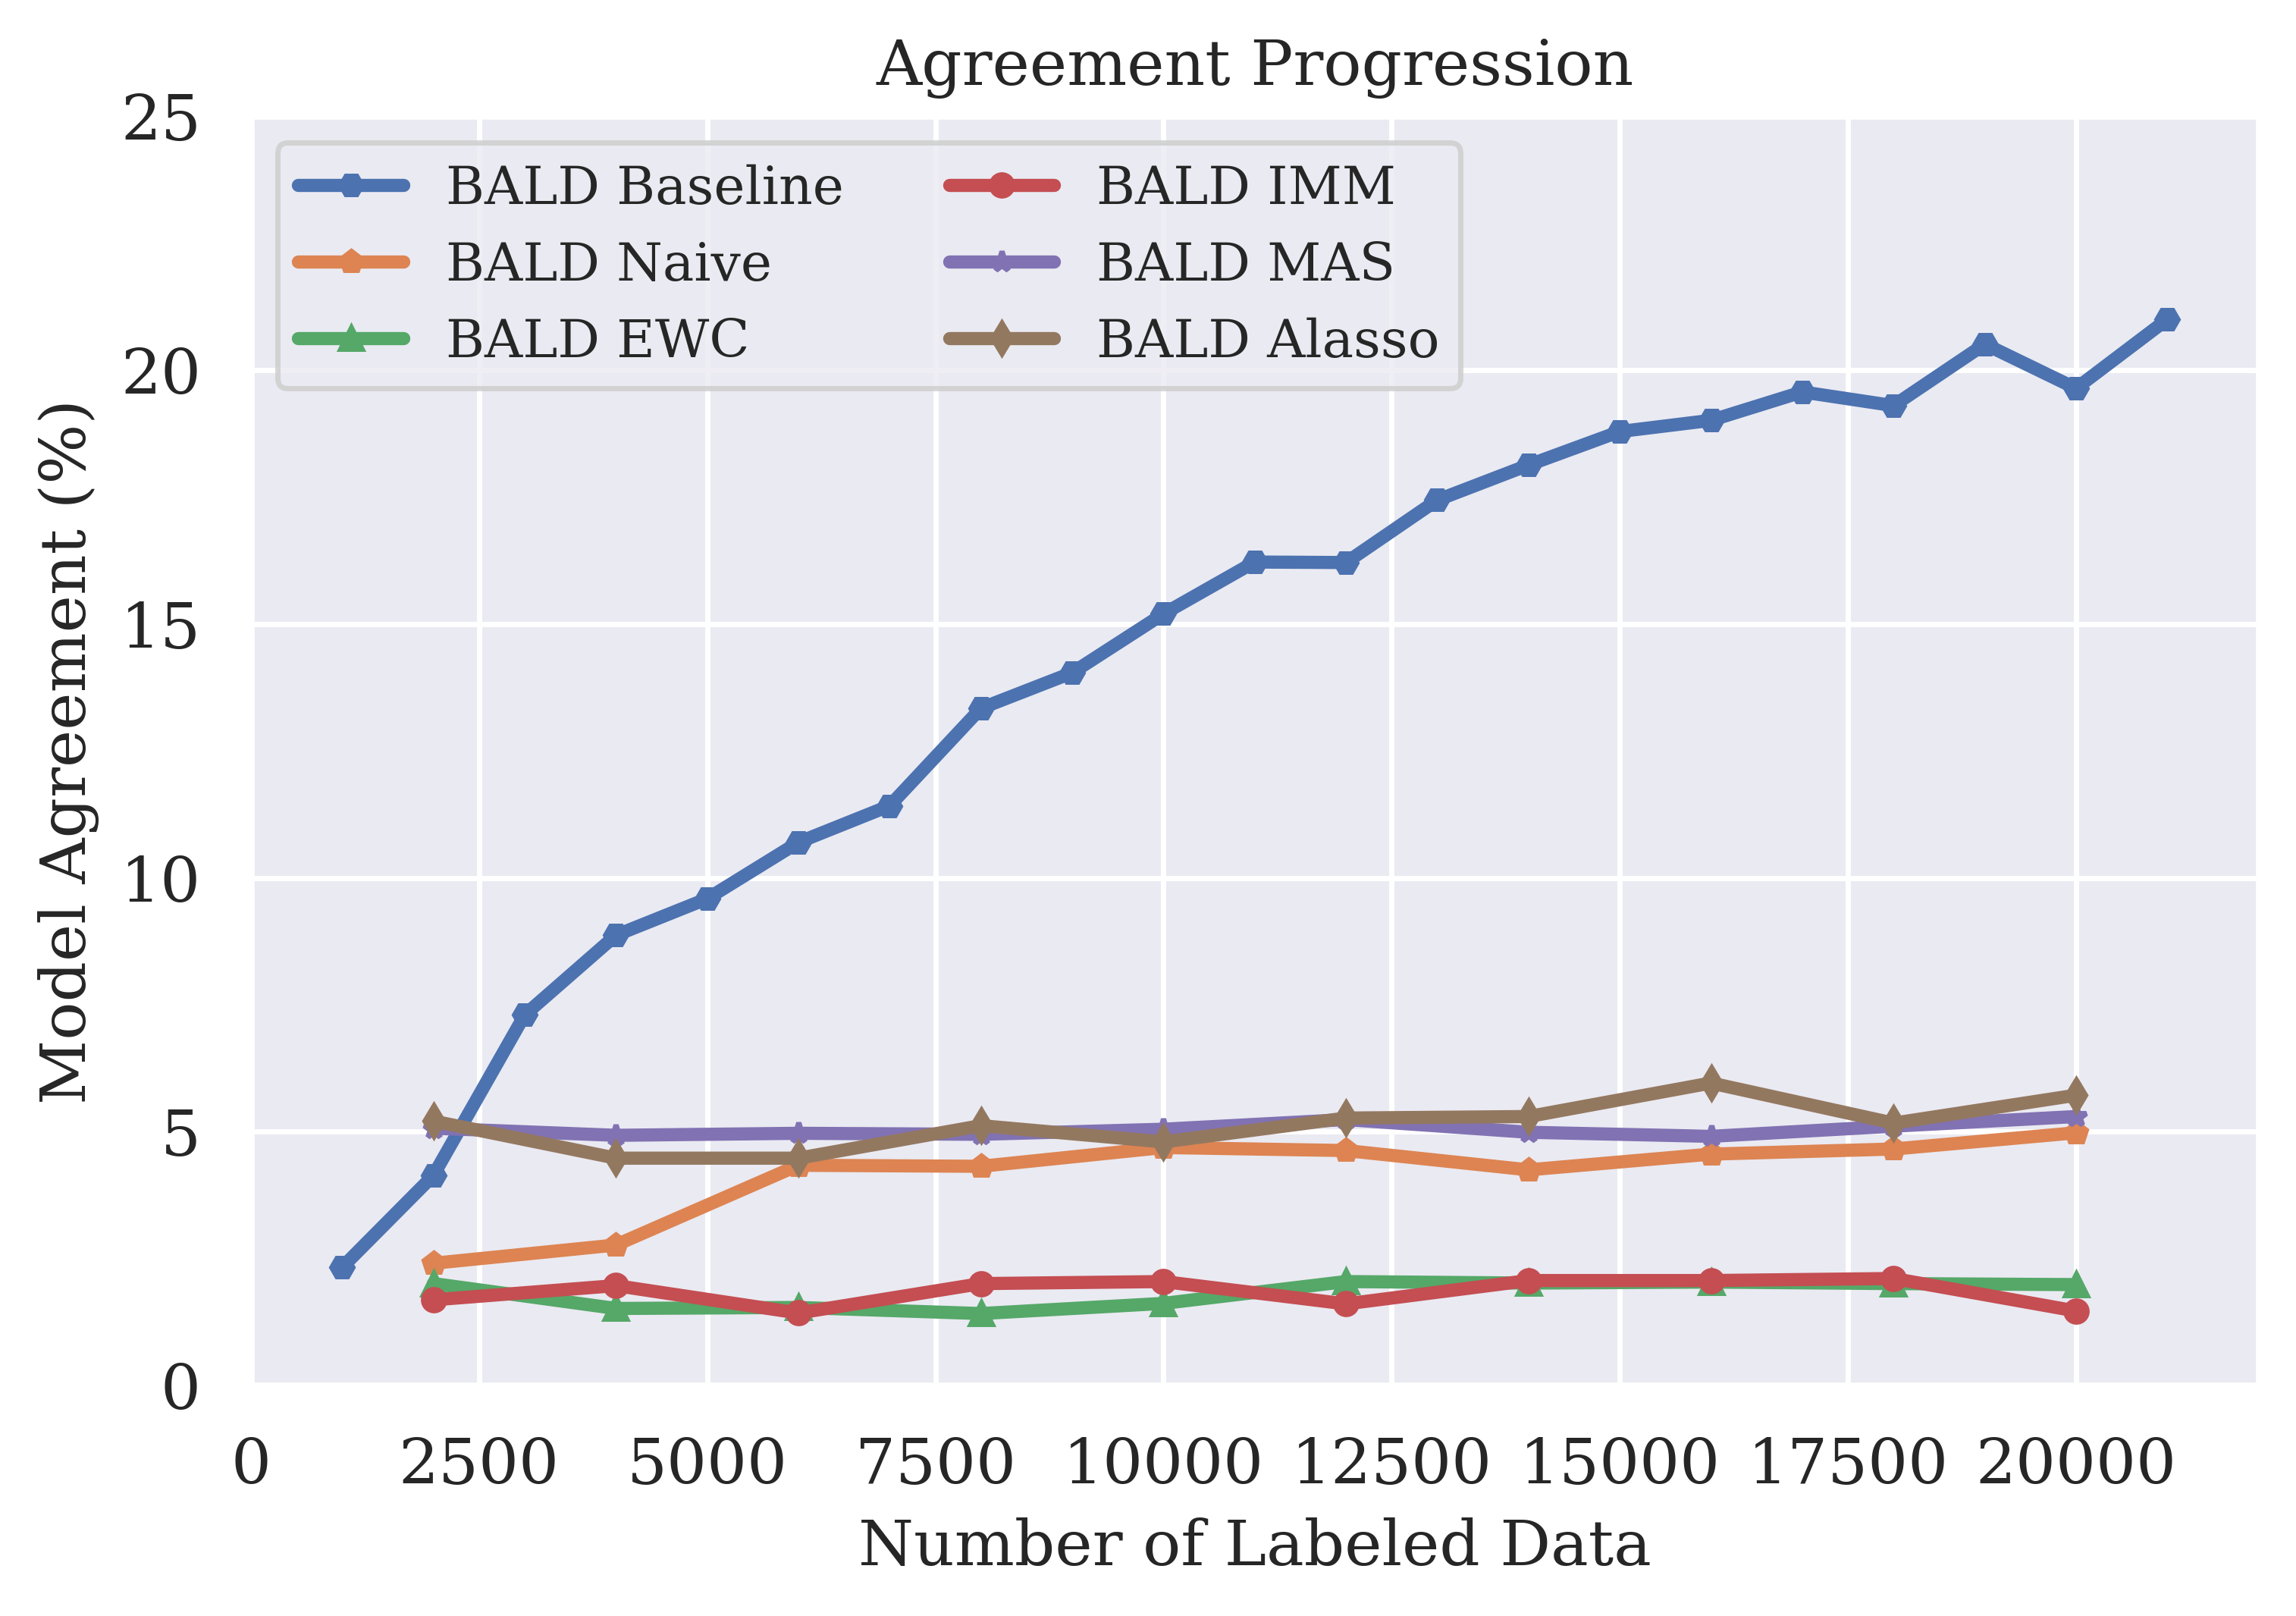
\includegraphics[width=0.7\linewidth]{images/results_CALMS/cifar100_label_bald.png}
    \caption[Agreement Comparison for Model Stealing on CIFAR100 using the predicted class label and the Active Learning strategy BALD]{Progression of Model
    Agreement (in \%) for Model Stealing Attacks using Continual Active Learning on the CIFAR-100 dataset. We use Model Stealing Attacks with the Active Learning
    strategy \gls{bald} and train using the predicted class label of the Target Model.}
    \label{fig:CALMSCIFAR100LabelBALD}
\end{figure}

\begin{figure}[h]
    \centering
    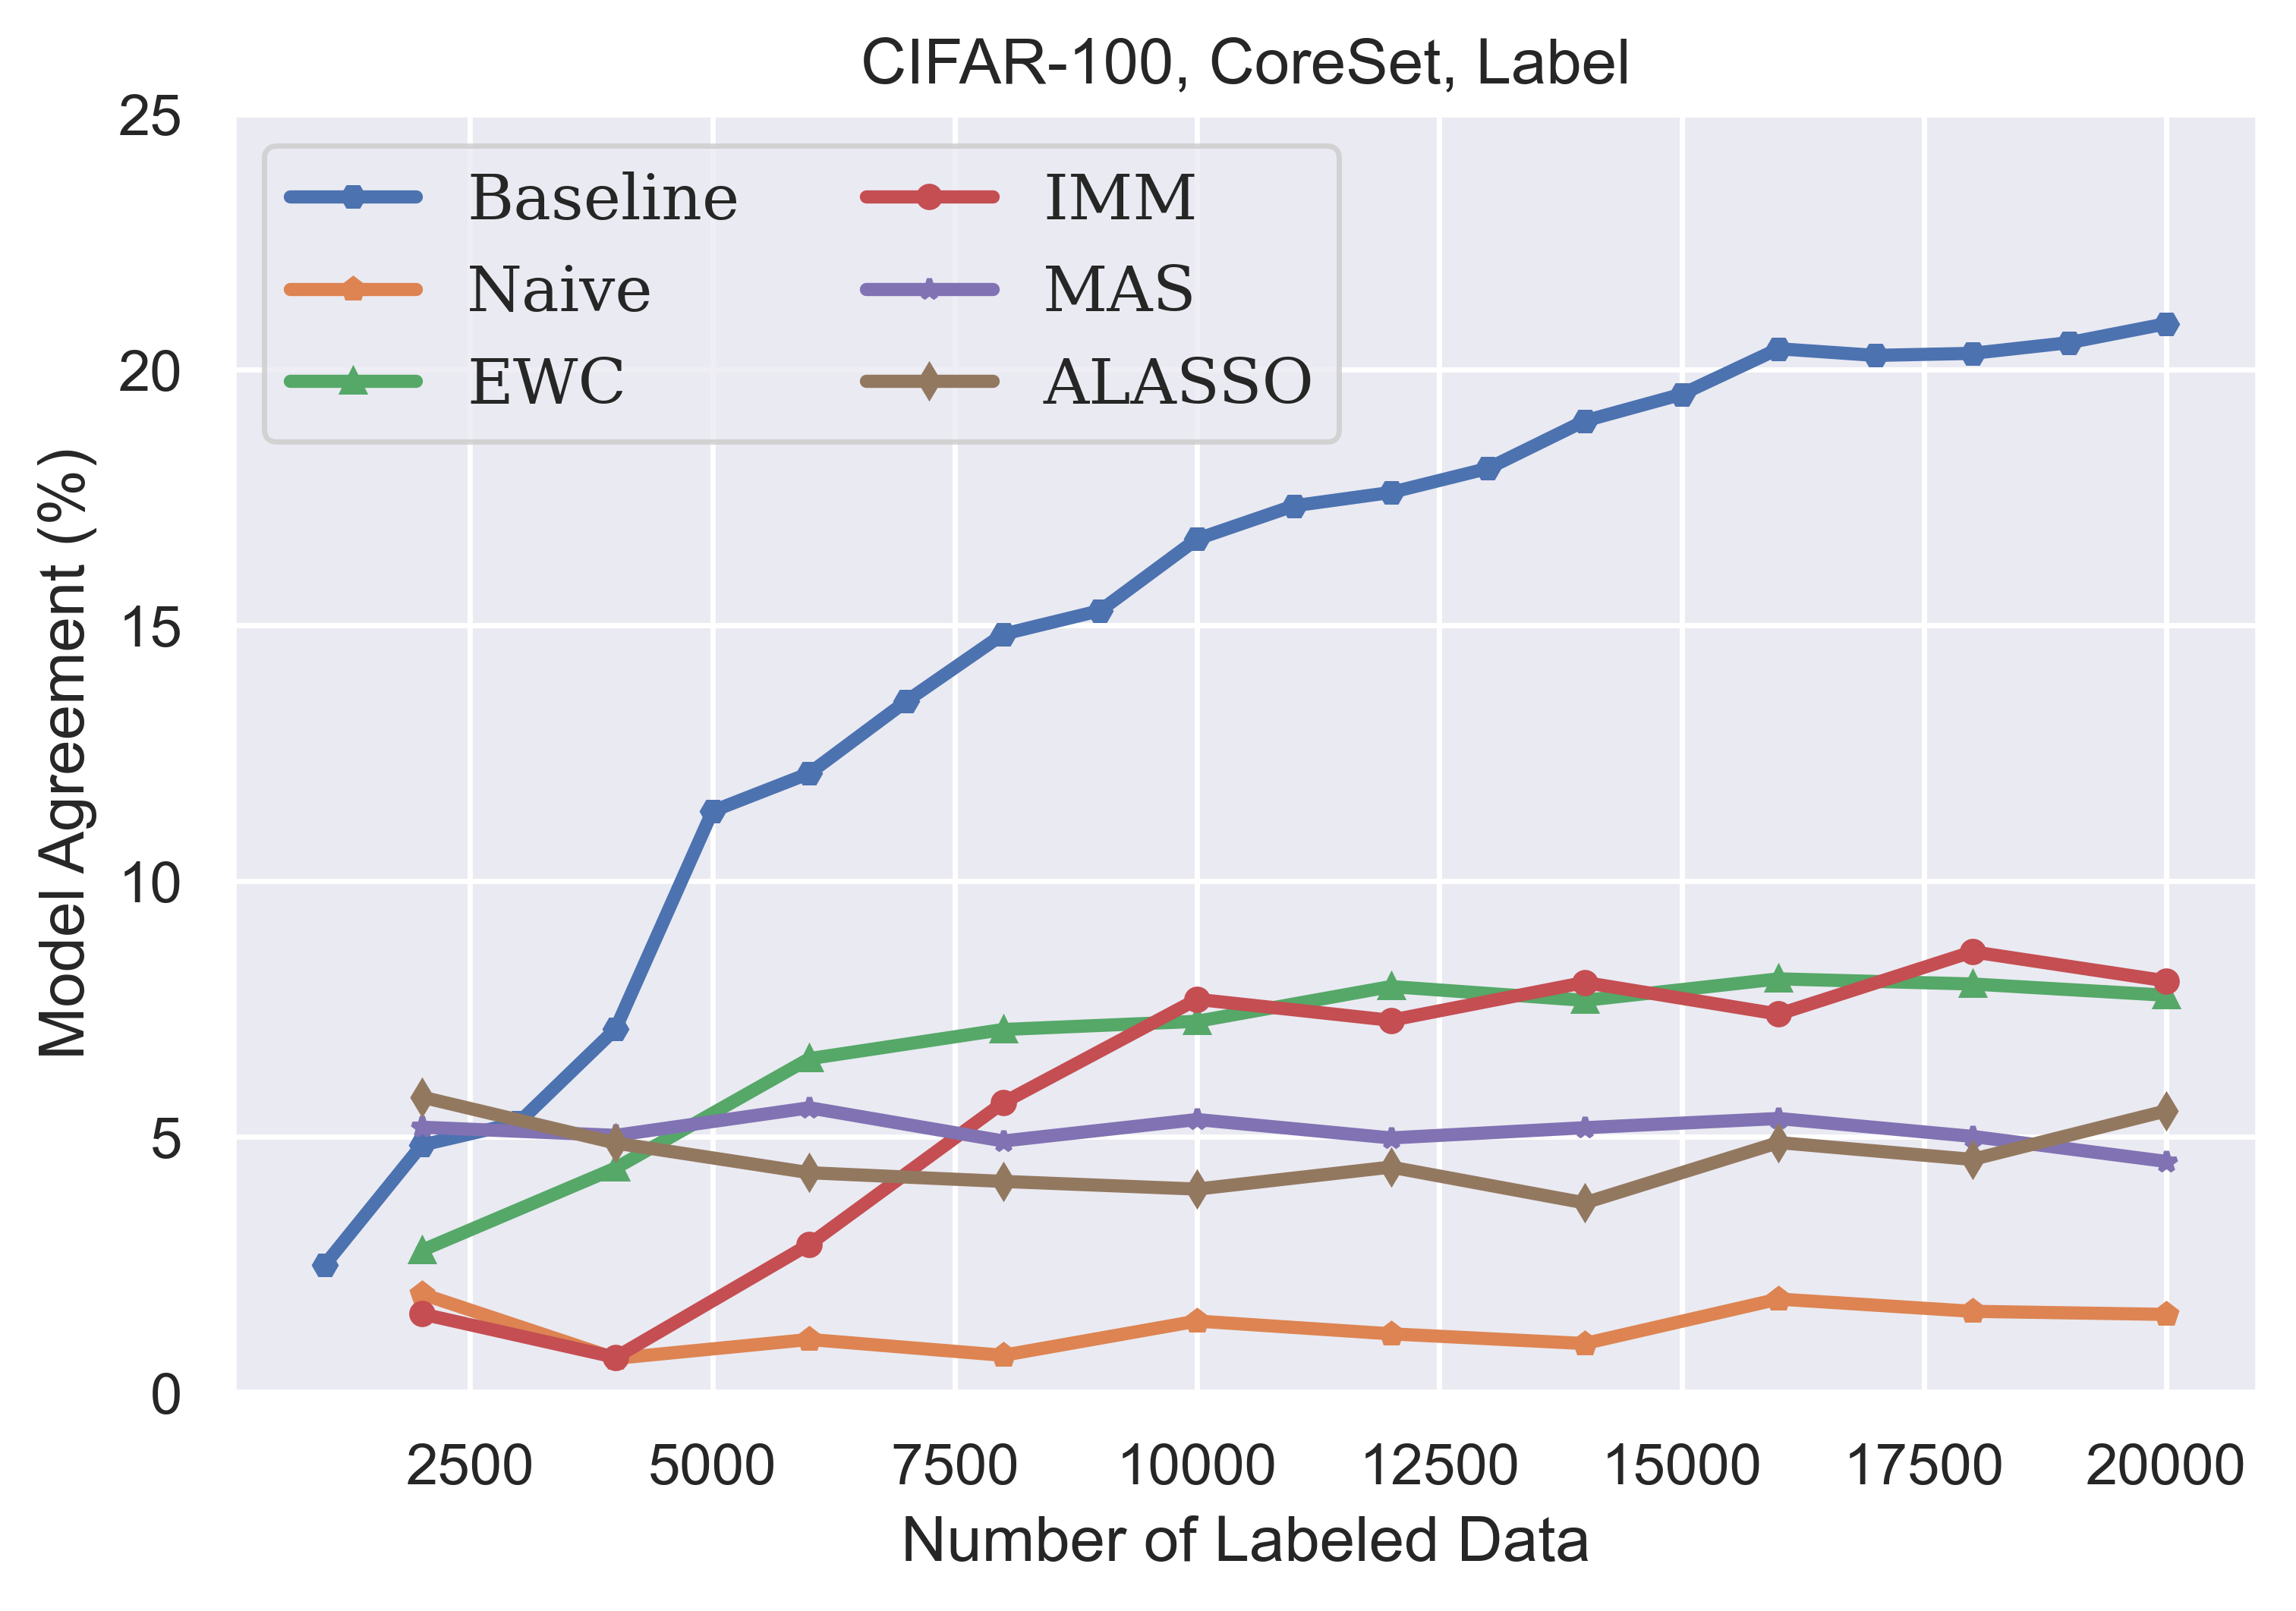
\includegraphics[width=0.7\linewidth]{images/results_CALMS/cifar100_label_coreset.png}
    \caption[Agreement Comparison for Model Stealing on CIFAR100 using the predicted class label and the Active Learning strategy CoreSet]{Progression of Model
    Agreement (in \%) for Model Stealing Attacks using Continual Active Learning on the CIFAR-100 dataset. We use Model Stealing Attacks with the Active Learning
    strategy CoreSet and train using the predicted class label of the Target Model.}
    \label{fig:CALMSCIFAR100LabelCoreSet}
\end{figure}


\begin{figure}[h]
    \centering
    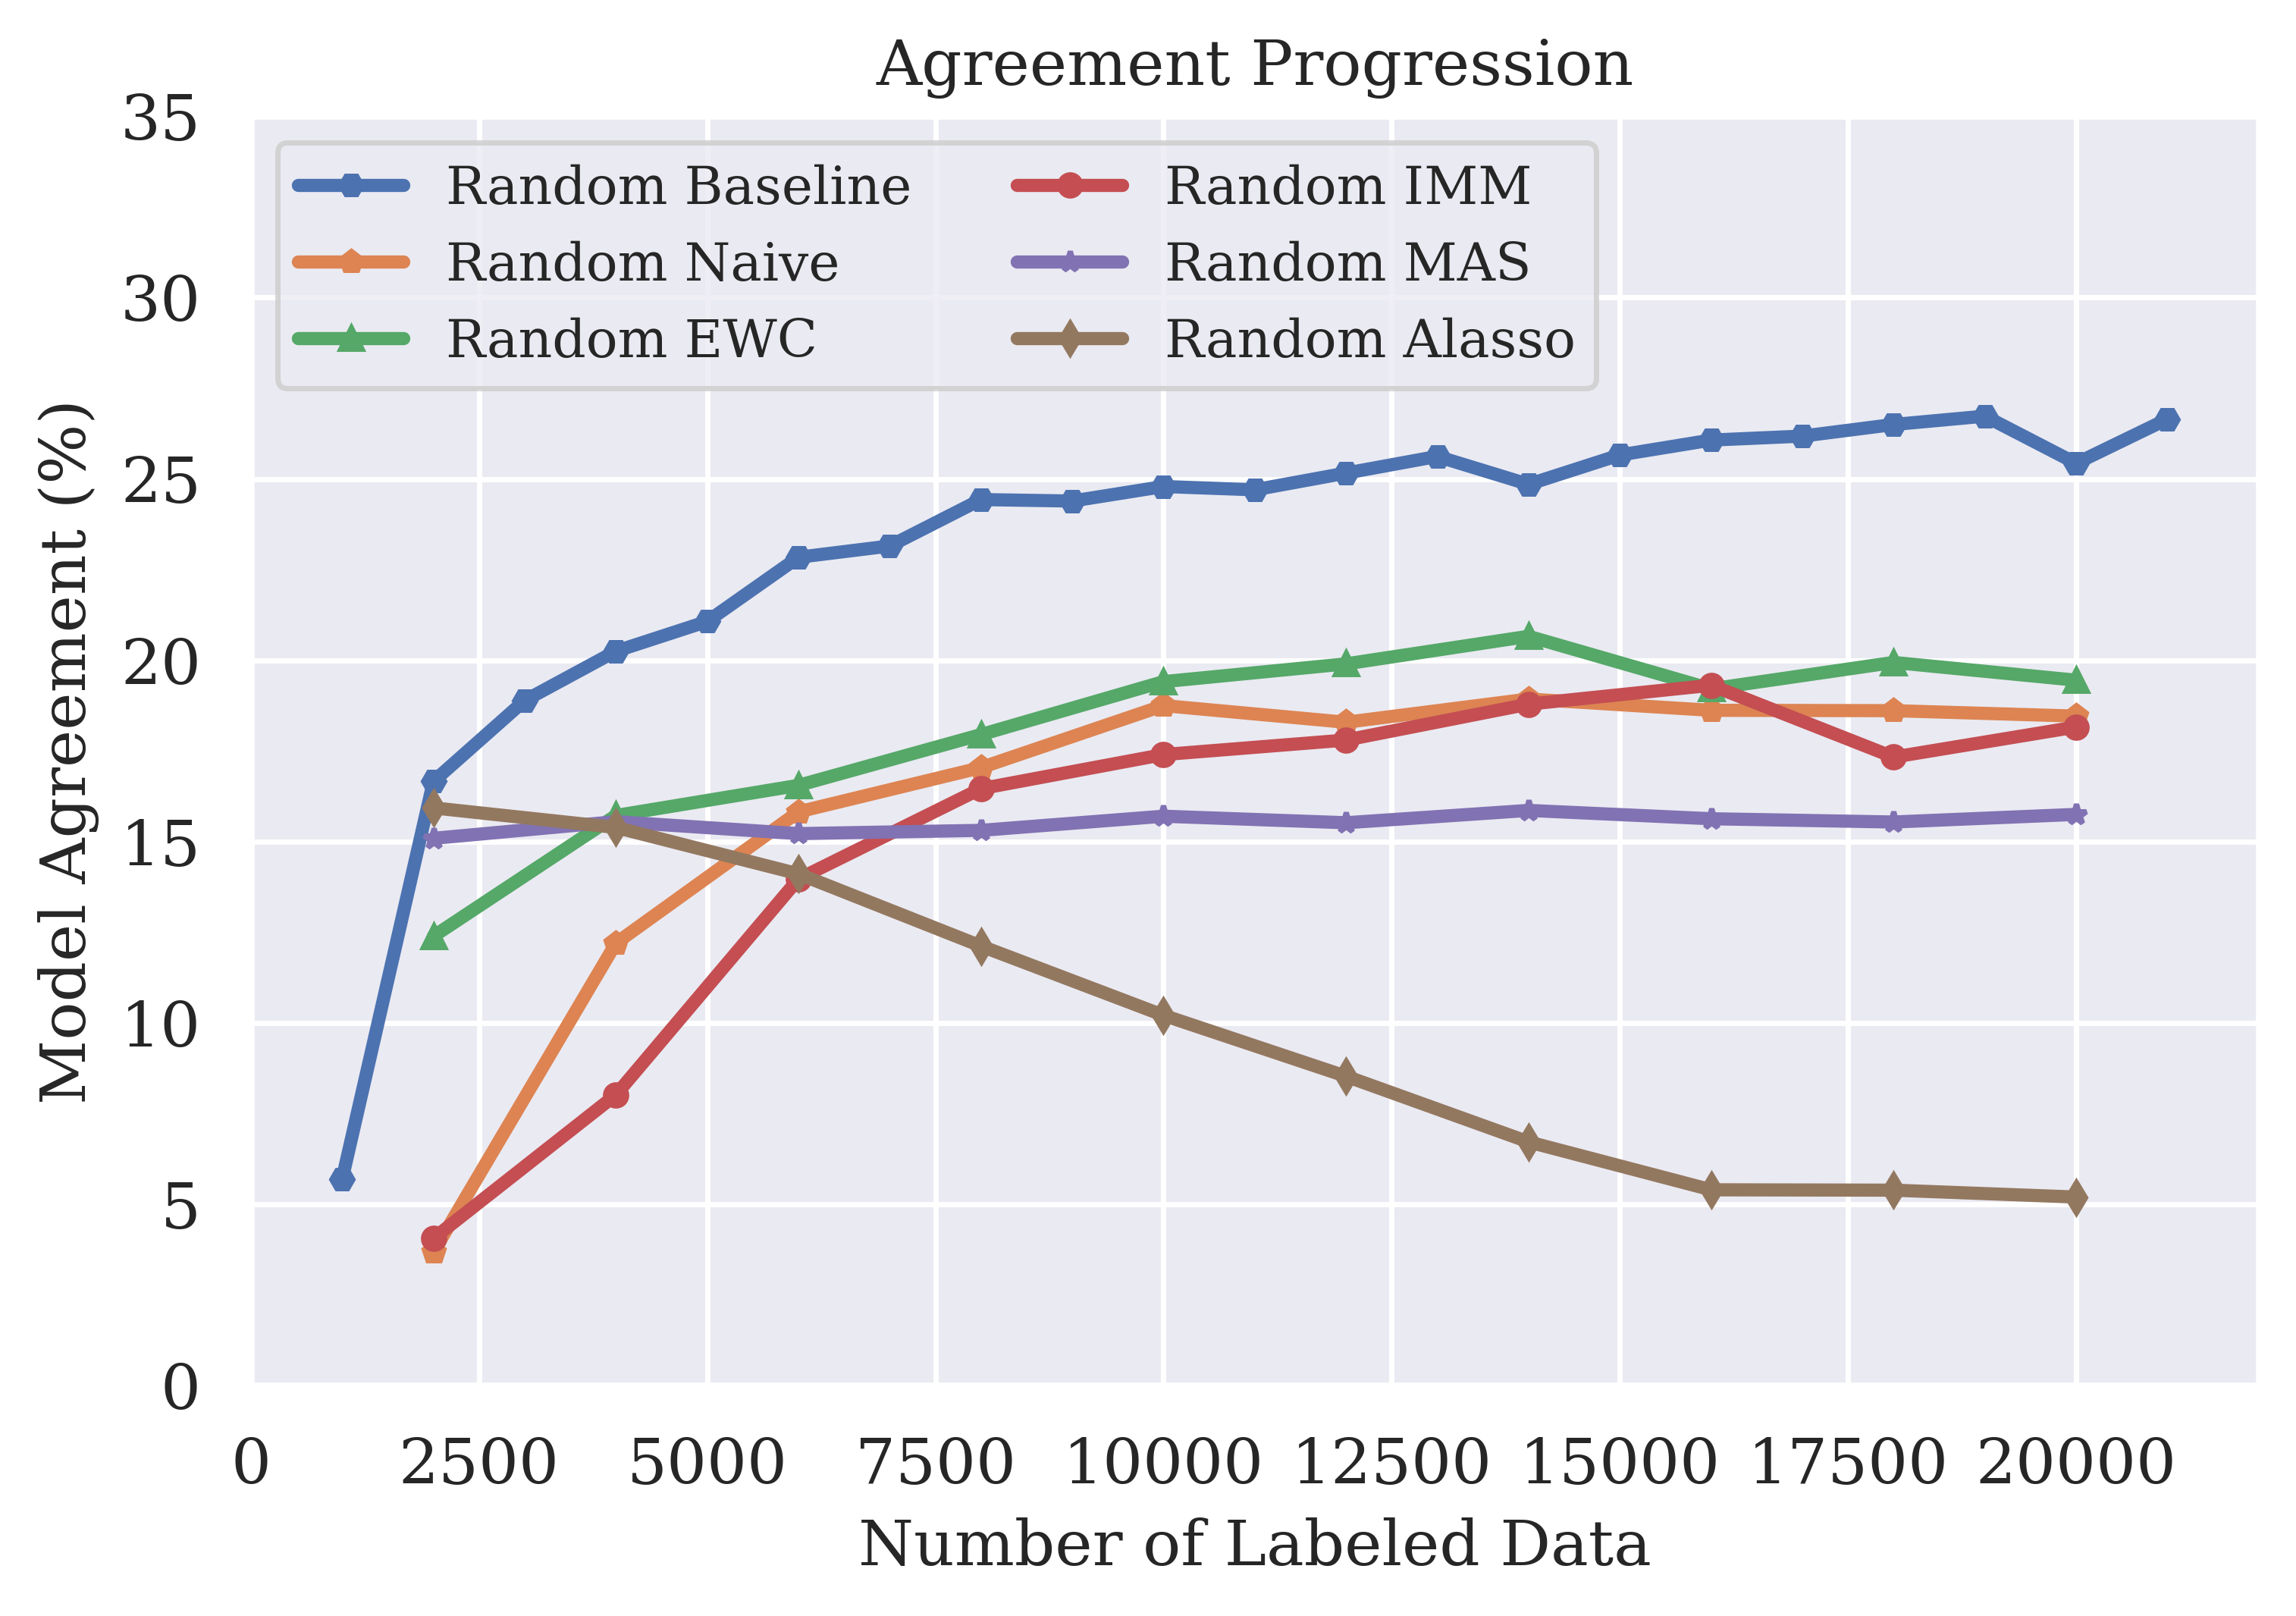
\includegraphics[width=0.7\linewidth]{images/results_CALMS/cifar100_softmax_random.png}
    \caption[Agreement Comparison for Model Stealing on CIFAR100 using the softmax output and the Active Learning strategy Random]{Progression of Model Agreement
    (in \%) for Model Stealing Attacks using Continual Active Learning on the MNIST dataset. We use Model Stealing Attacks with random sampling
    and train using the softmax output of the Target Model.}
    \label{fig:CALMSCIFAR100SoftmaxRandom}
\end{figure}

\begin{figure}[h]
    \centering
    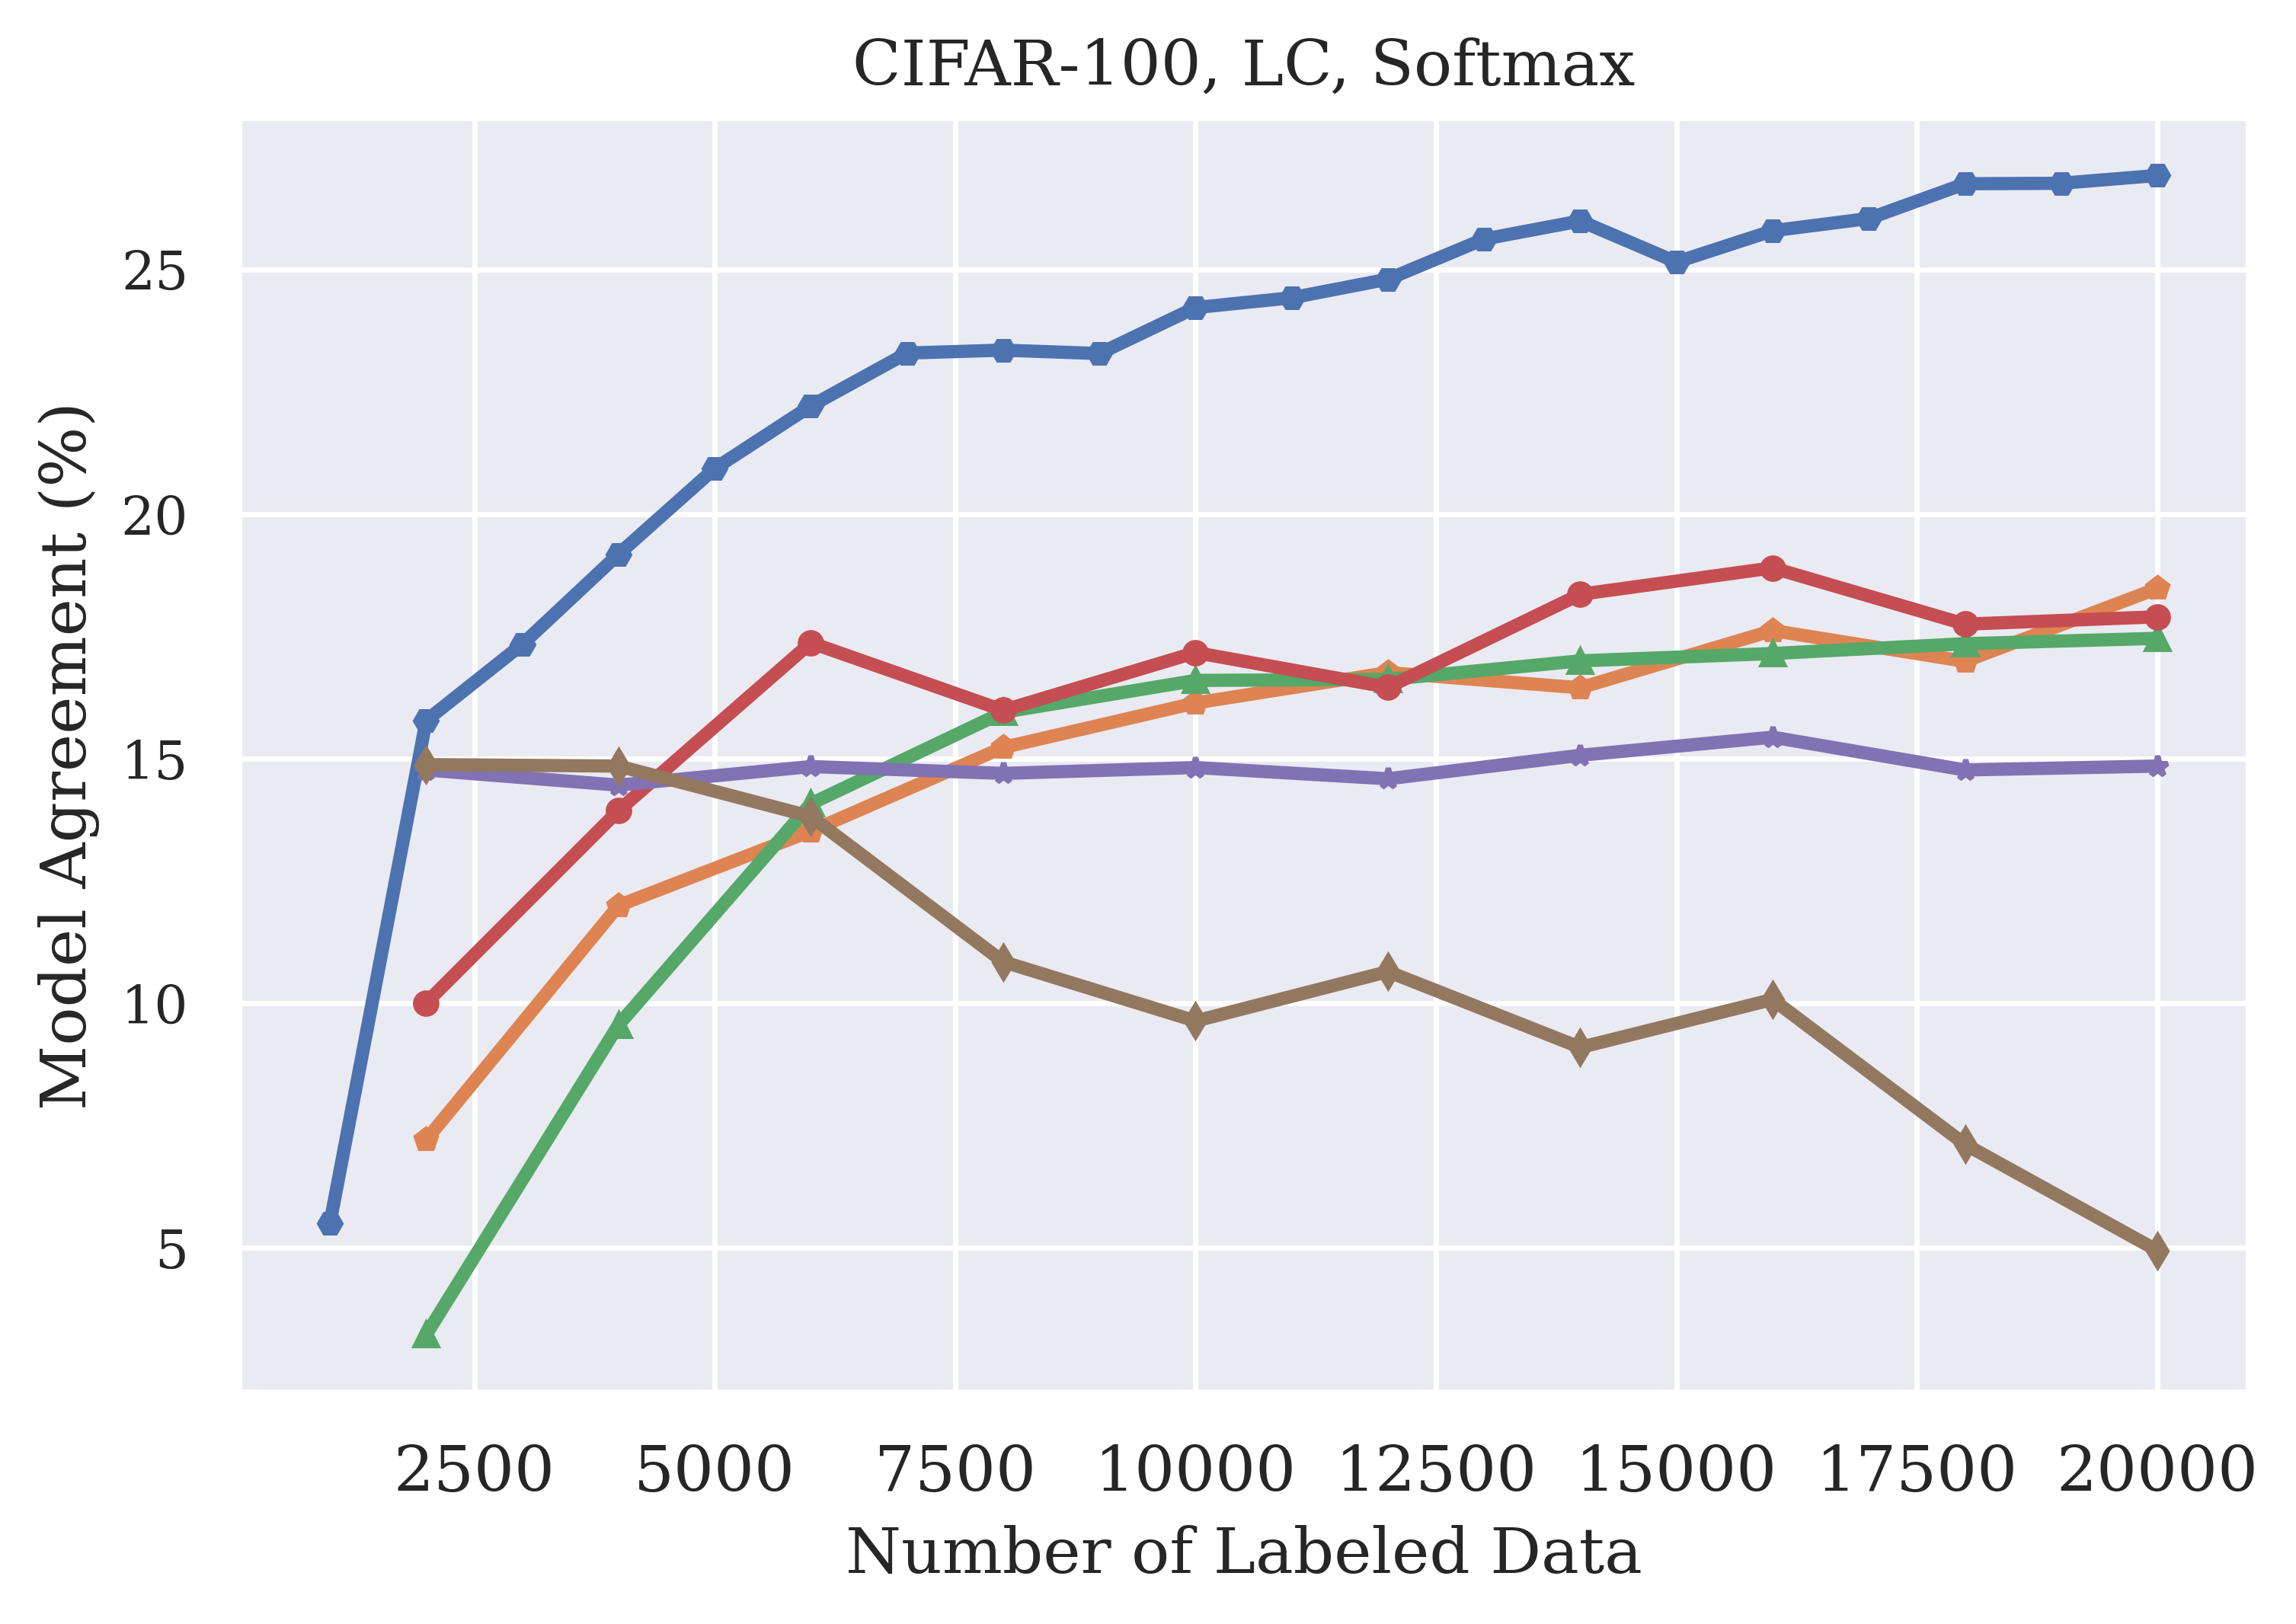
\includegraphics[width=0.7\linewidth]{images/results_CALMS/cifar100_softmax_lc.png}
    \caption[Agreement Comparison for Model Stealing on CIFAR100 using the softmax output and the Active Learning strategy LC]{Progression of Model Agreement
    (in \%) for Model Stealing Attacks using Continual Active Learning on the MNIST dataset. We use Model Stealing Attacks with the Active Learning strategy
    \gls{lc} and train using the softmax output of the Target Model.}
    \label{fig:CALMSCIFAR100SoftmaxLC}
\end{figure}

\begin{figure}[h]
    \centering
    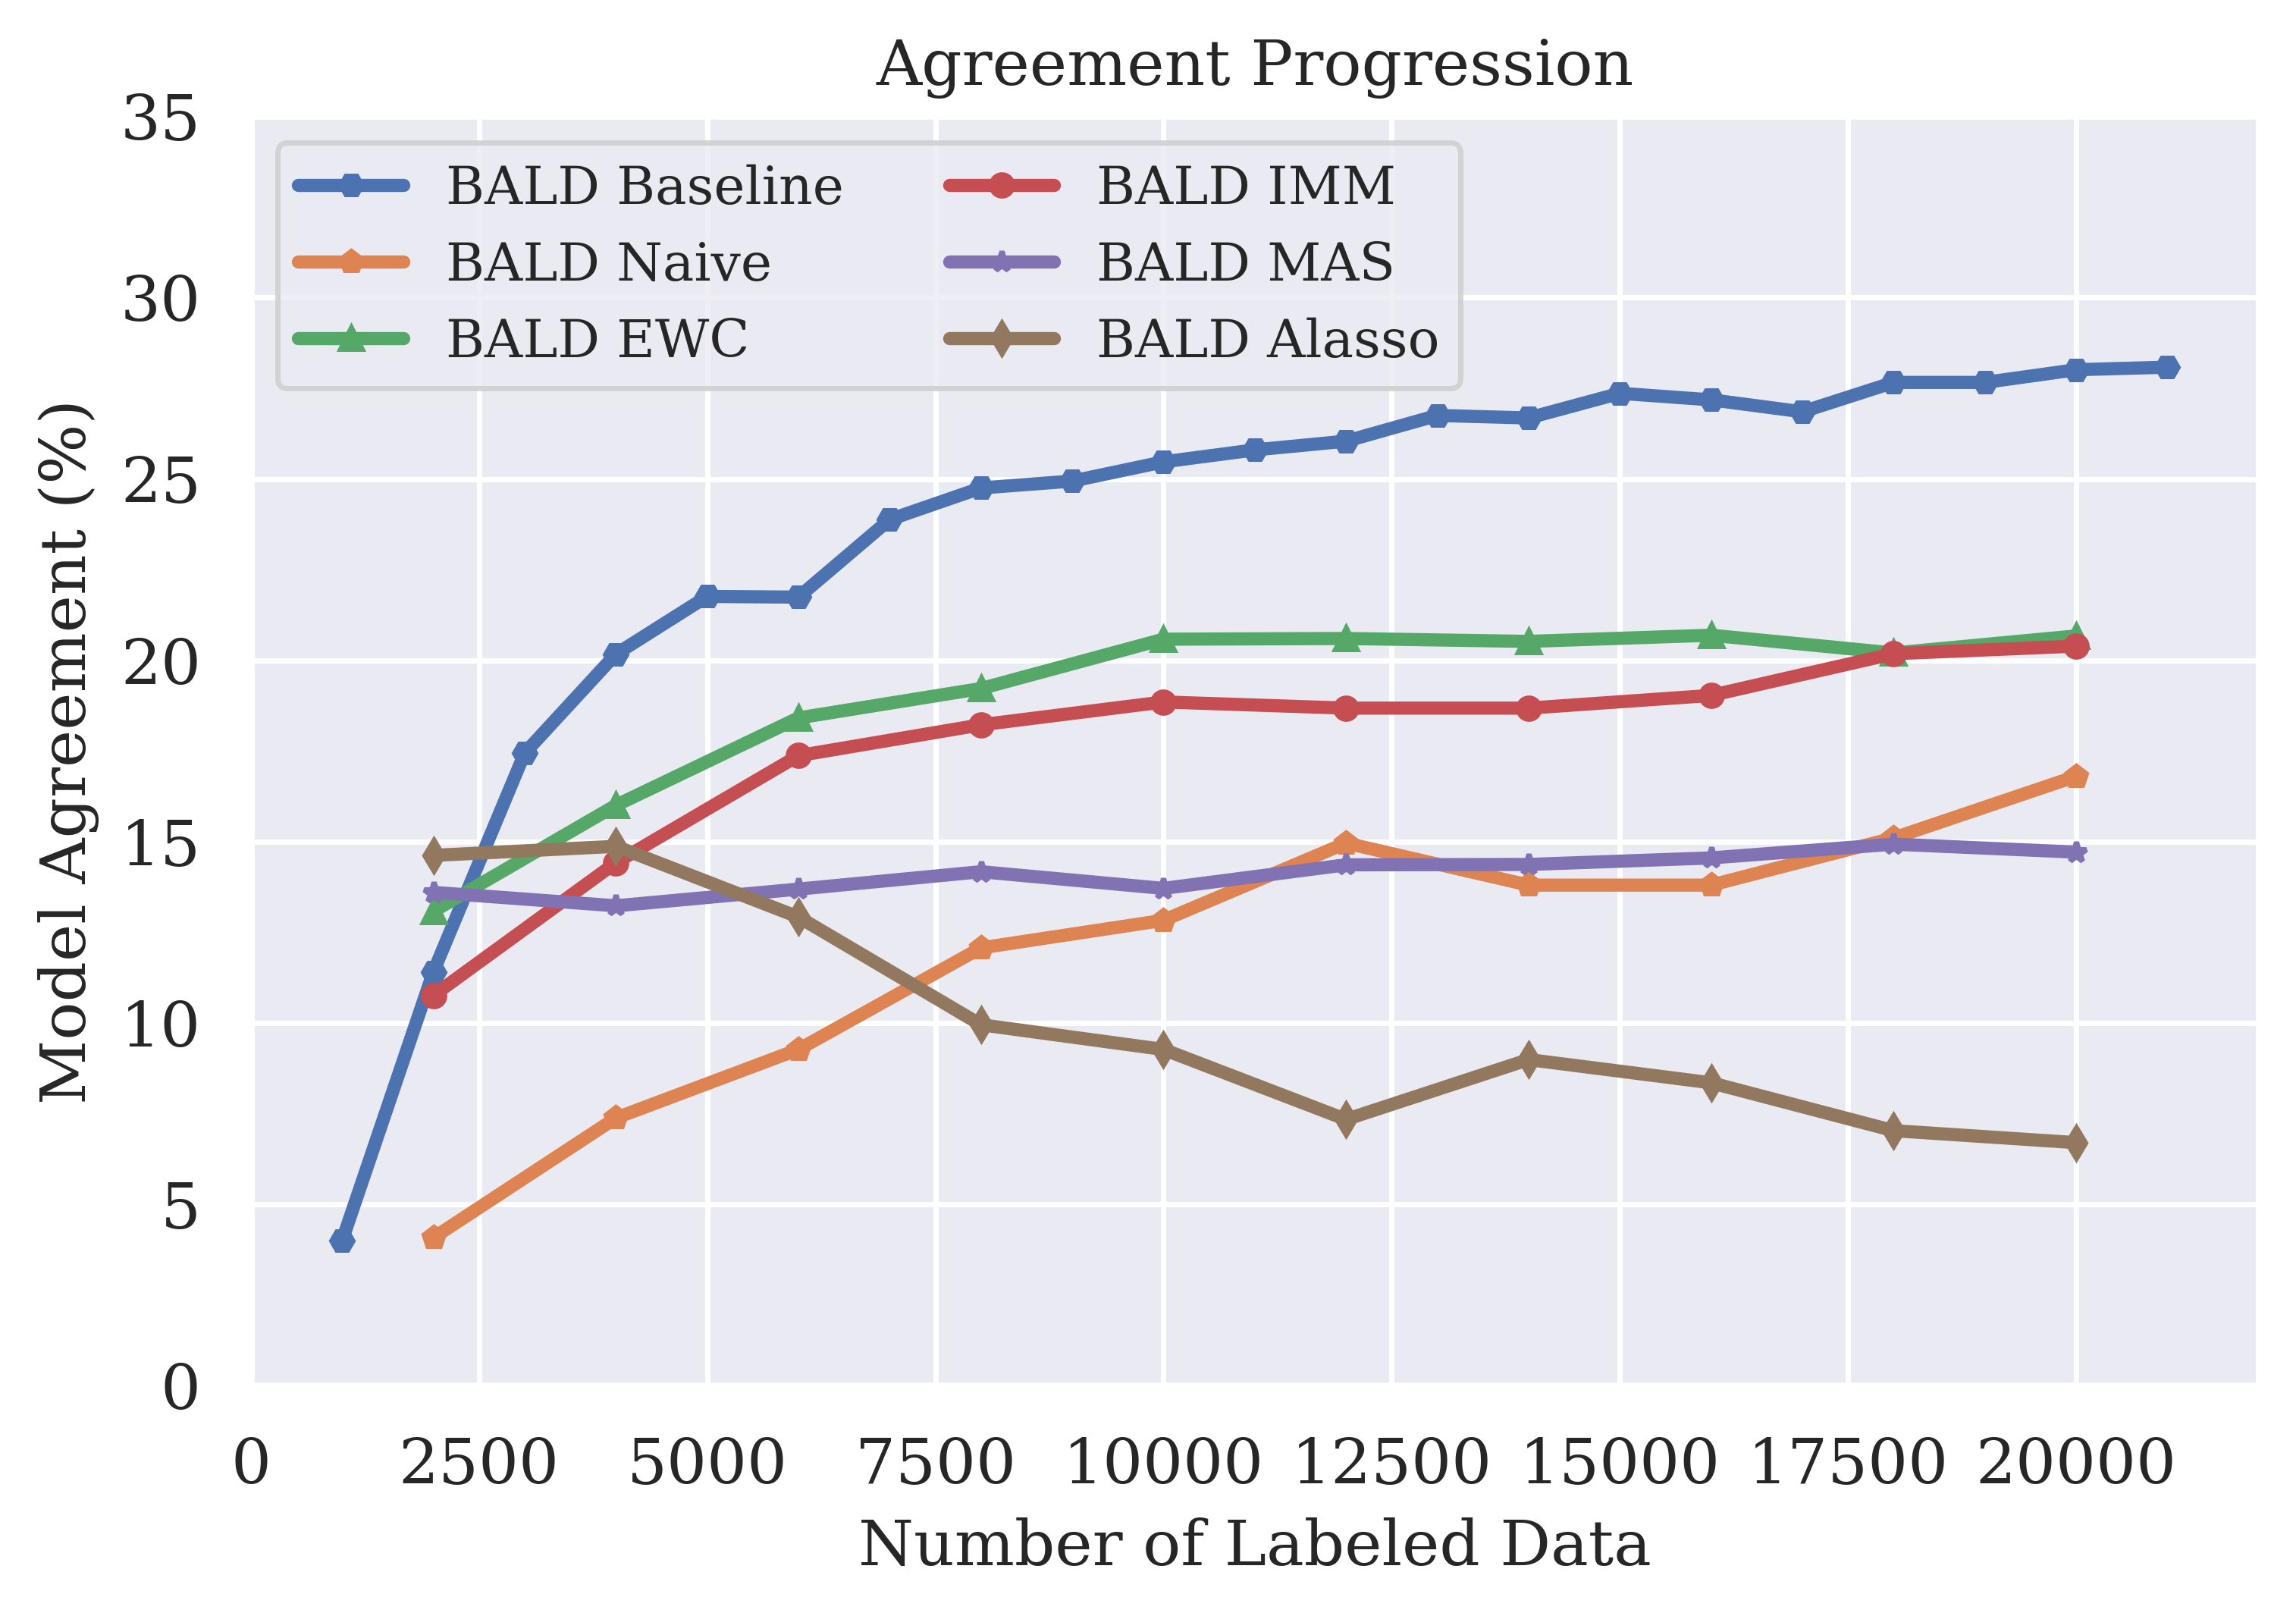
\includegraphics[width=0.7\linewidth]{images/results_CALMS/cifar100_softmax_bald.png}
    \caption[Agreement Comparison for Model Stealing on CIFAR100 using the softmax output and the Active Learning strategy BALD]{Progression of Model Agreement
    (in \%) for Model Stealing Attacks using Continual Active Learning on the MNIST dataset. We use Model Stealing Attacks with the Active Learning strategy
    \gls{bald} and train using the softmax output of the Target Model.}
    \label{fig:CALMSCIFAR100SoftmaxBALD}
\end{figure}

\begin{figure}[h]
    \centering
    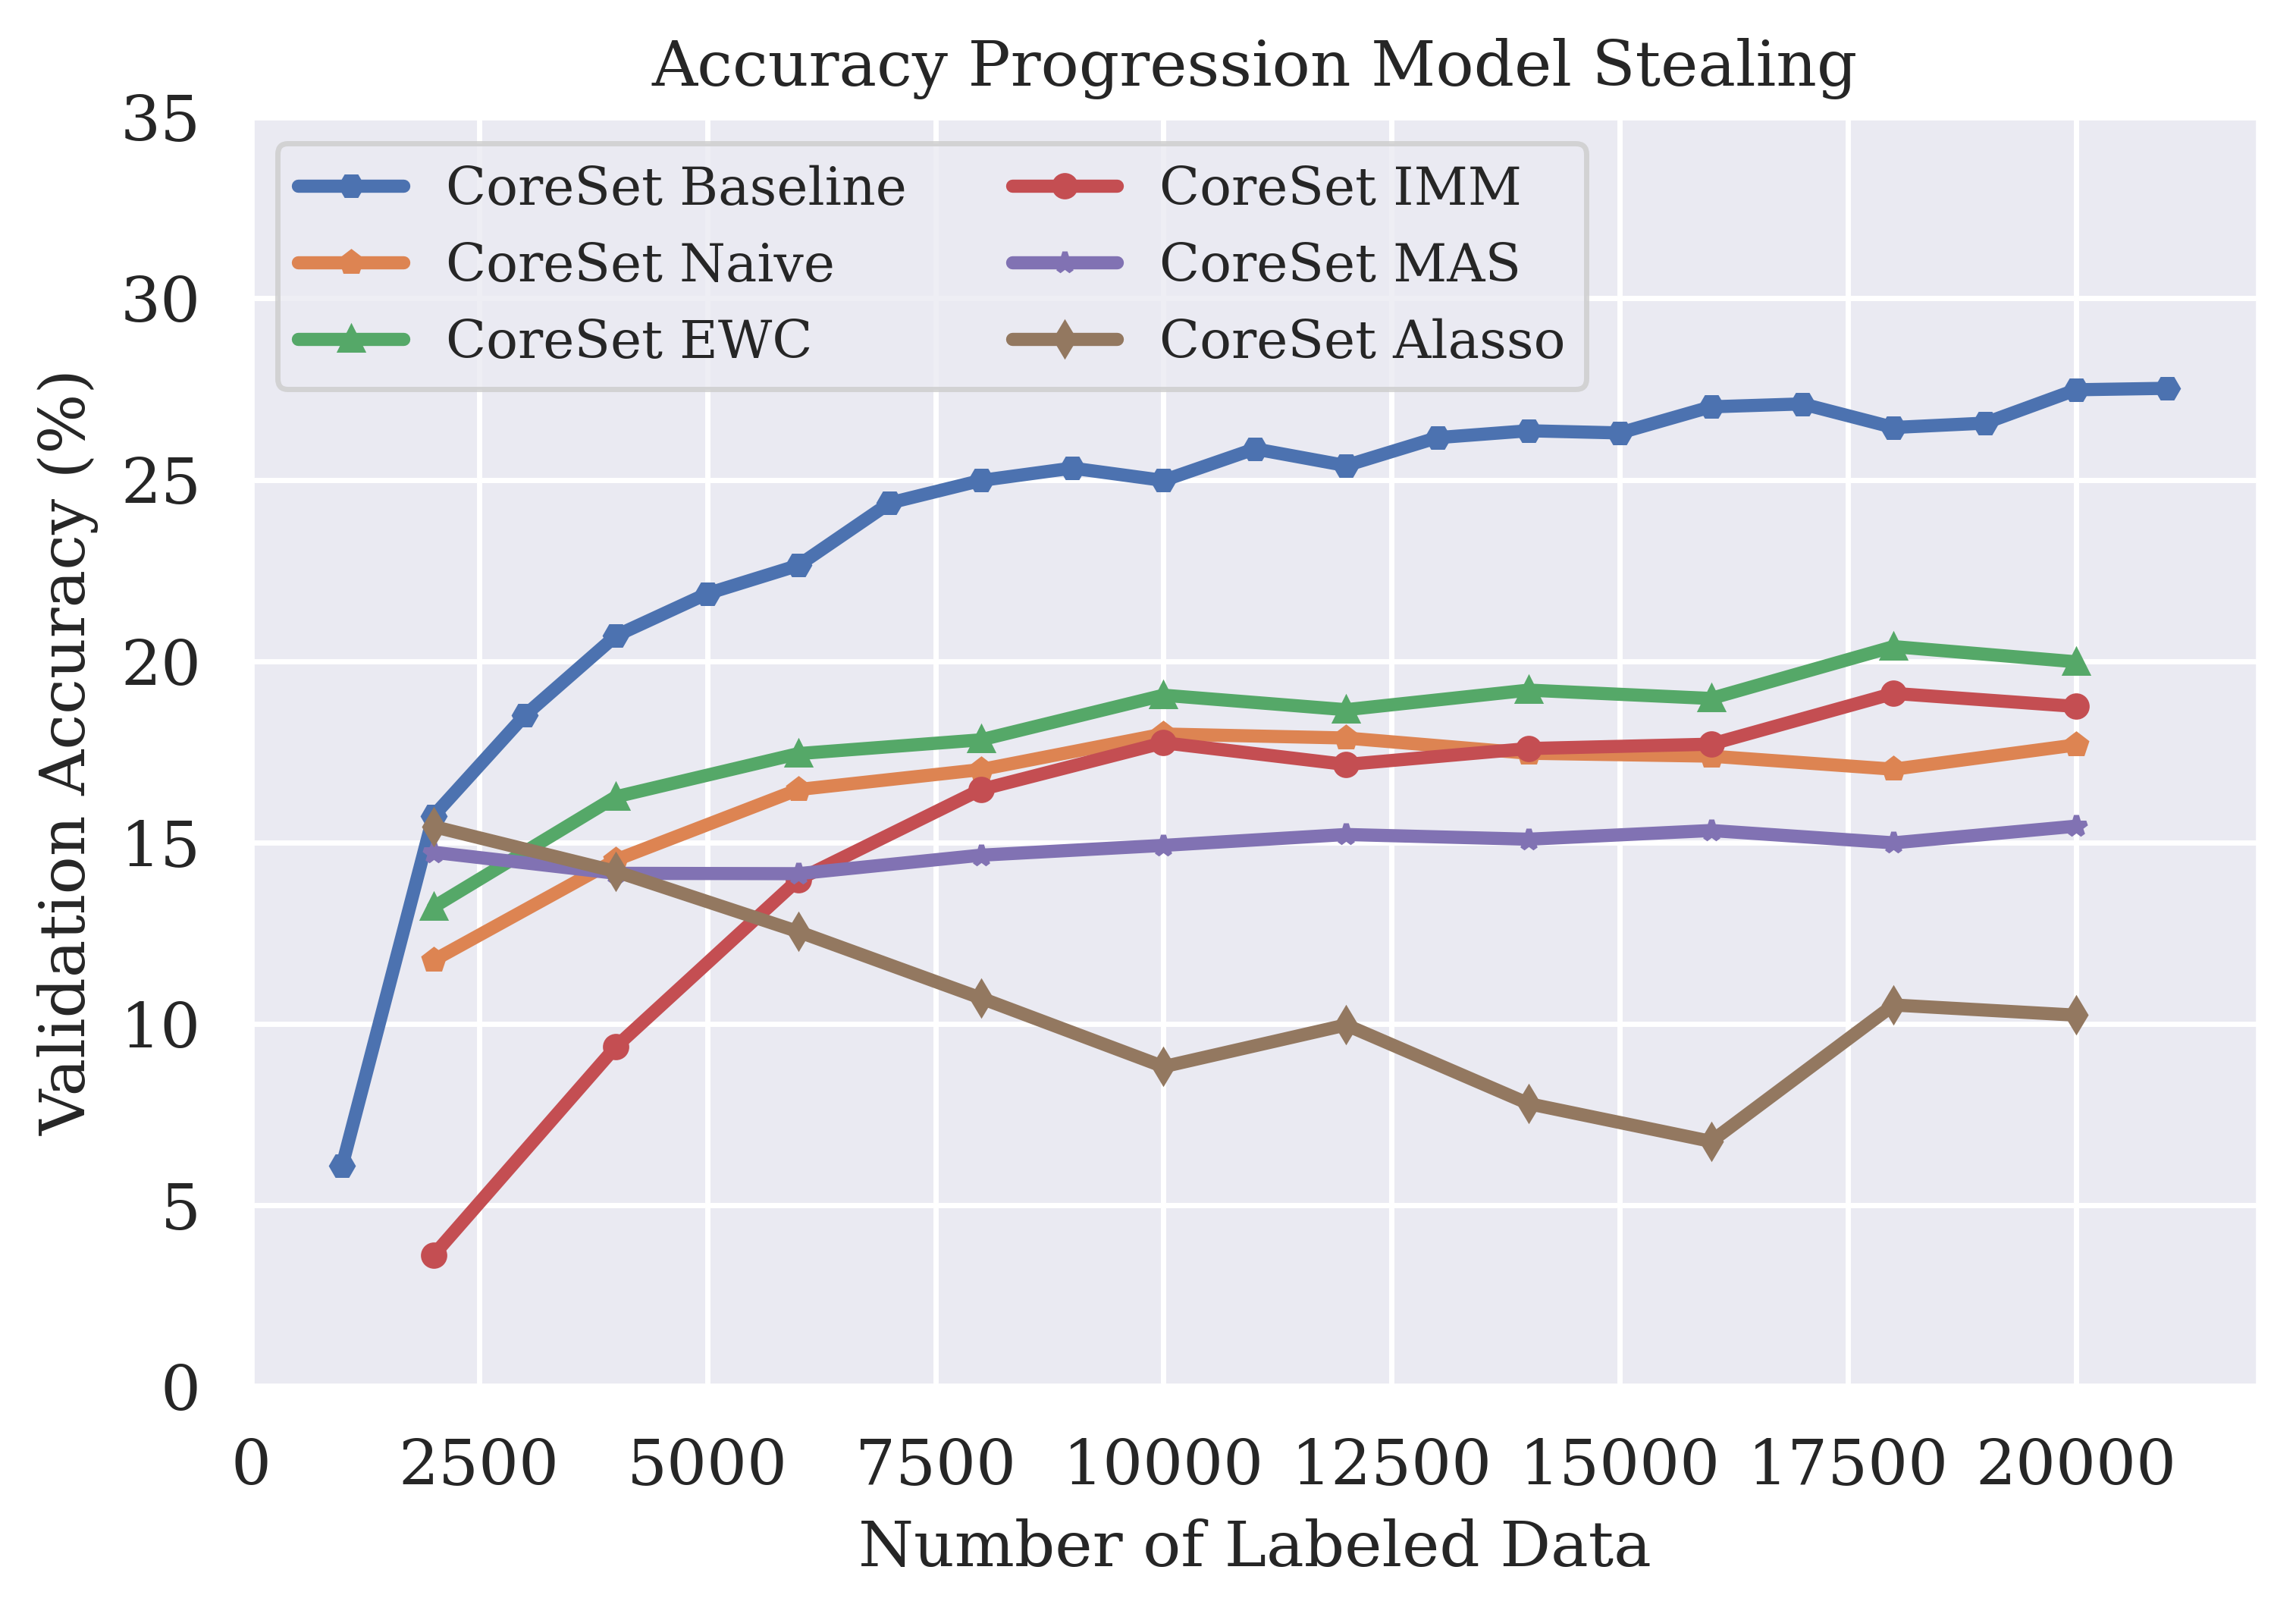
\includegraphics[width=0.7\linewidth]{images/results_CALMS/cifar100_softmax_coreset.png}
    \caption[Agreement Comparison for Model Stealing on CIFAR100 using the softmax output and the Active Learning strategy CoreSet]{Progression of Model Agreement
    (in \%) for Model Stealing Attacks using Continual Active Learning on the MNIST dataset. We use Model Stealing Attacks with the Active Learning strategy
    CoreSet and train using the softmax output of the Target Model.}
    \label{fig:CALMSCIFAR100SoftmaxCoreSet}
\end{figure}

%Tables for Cifar10
%Label
\begin{figure}[h]
    \centering
    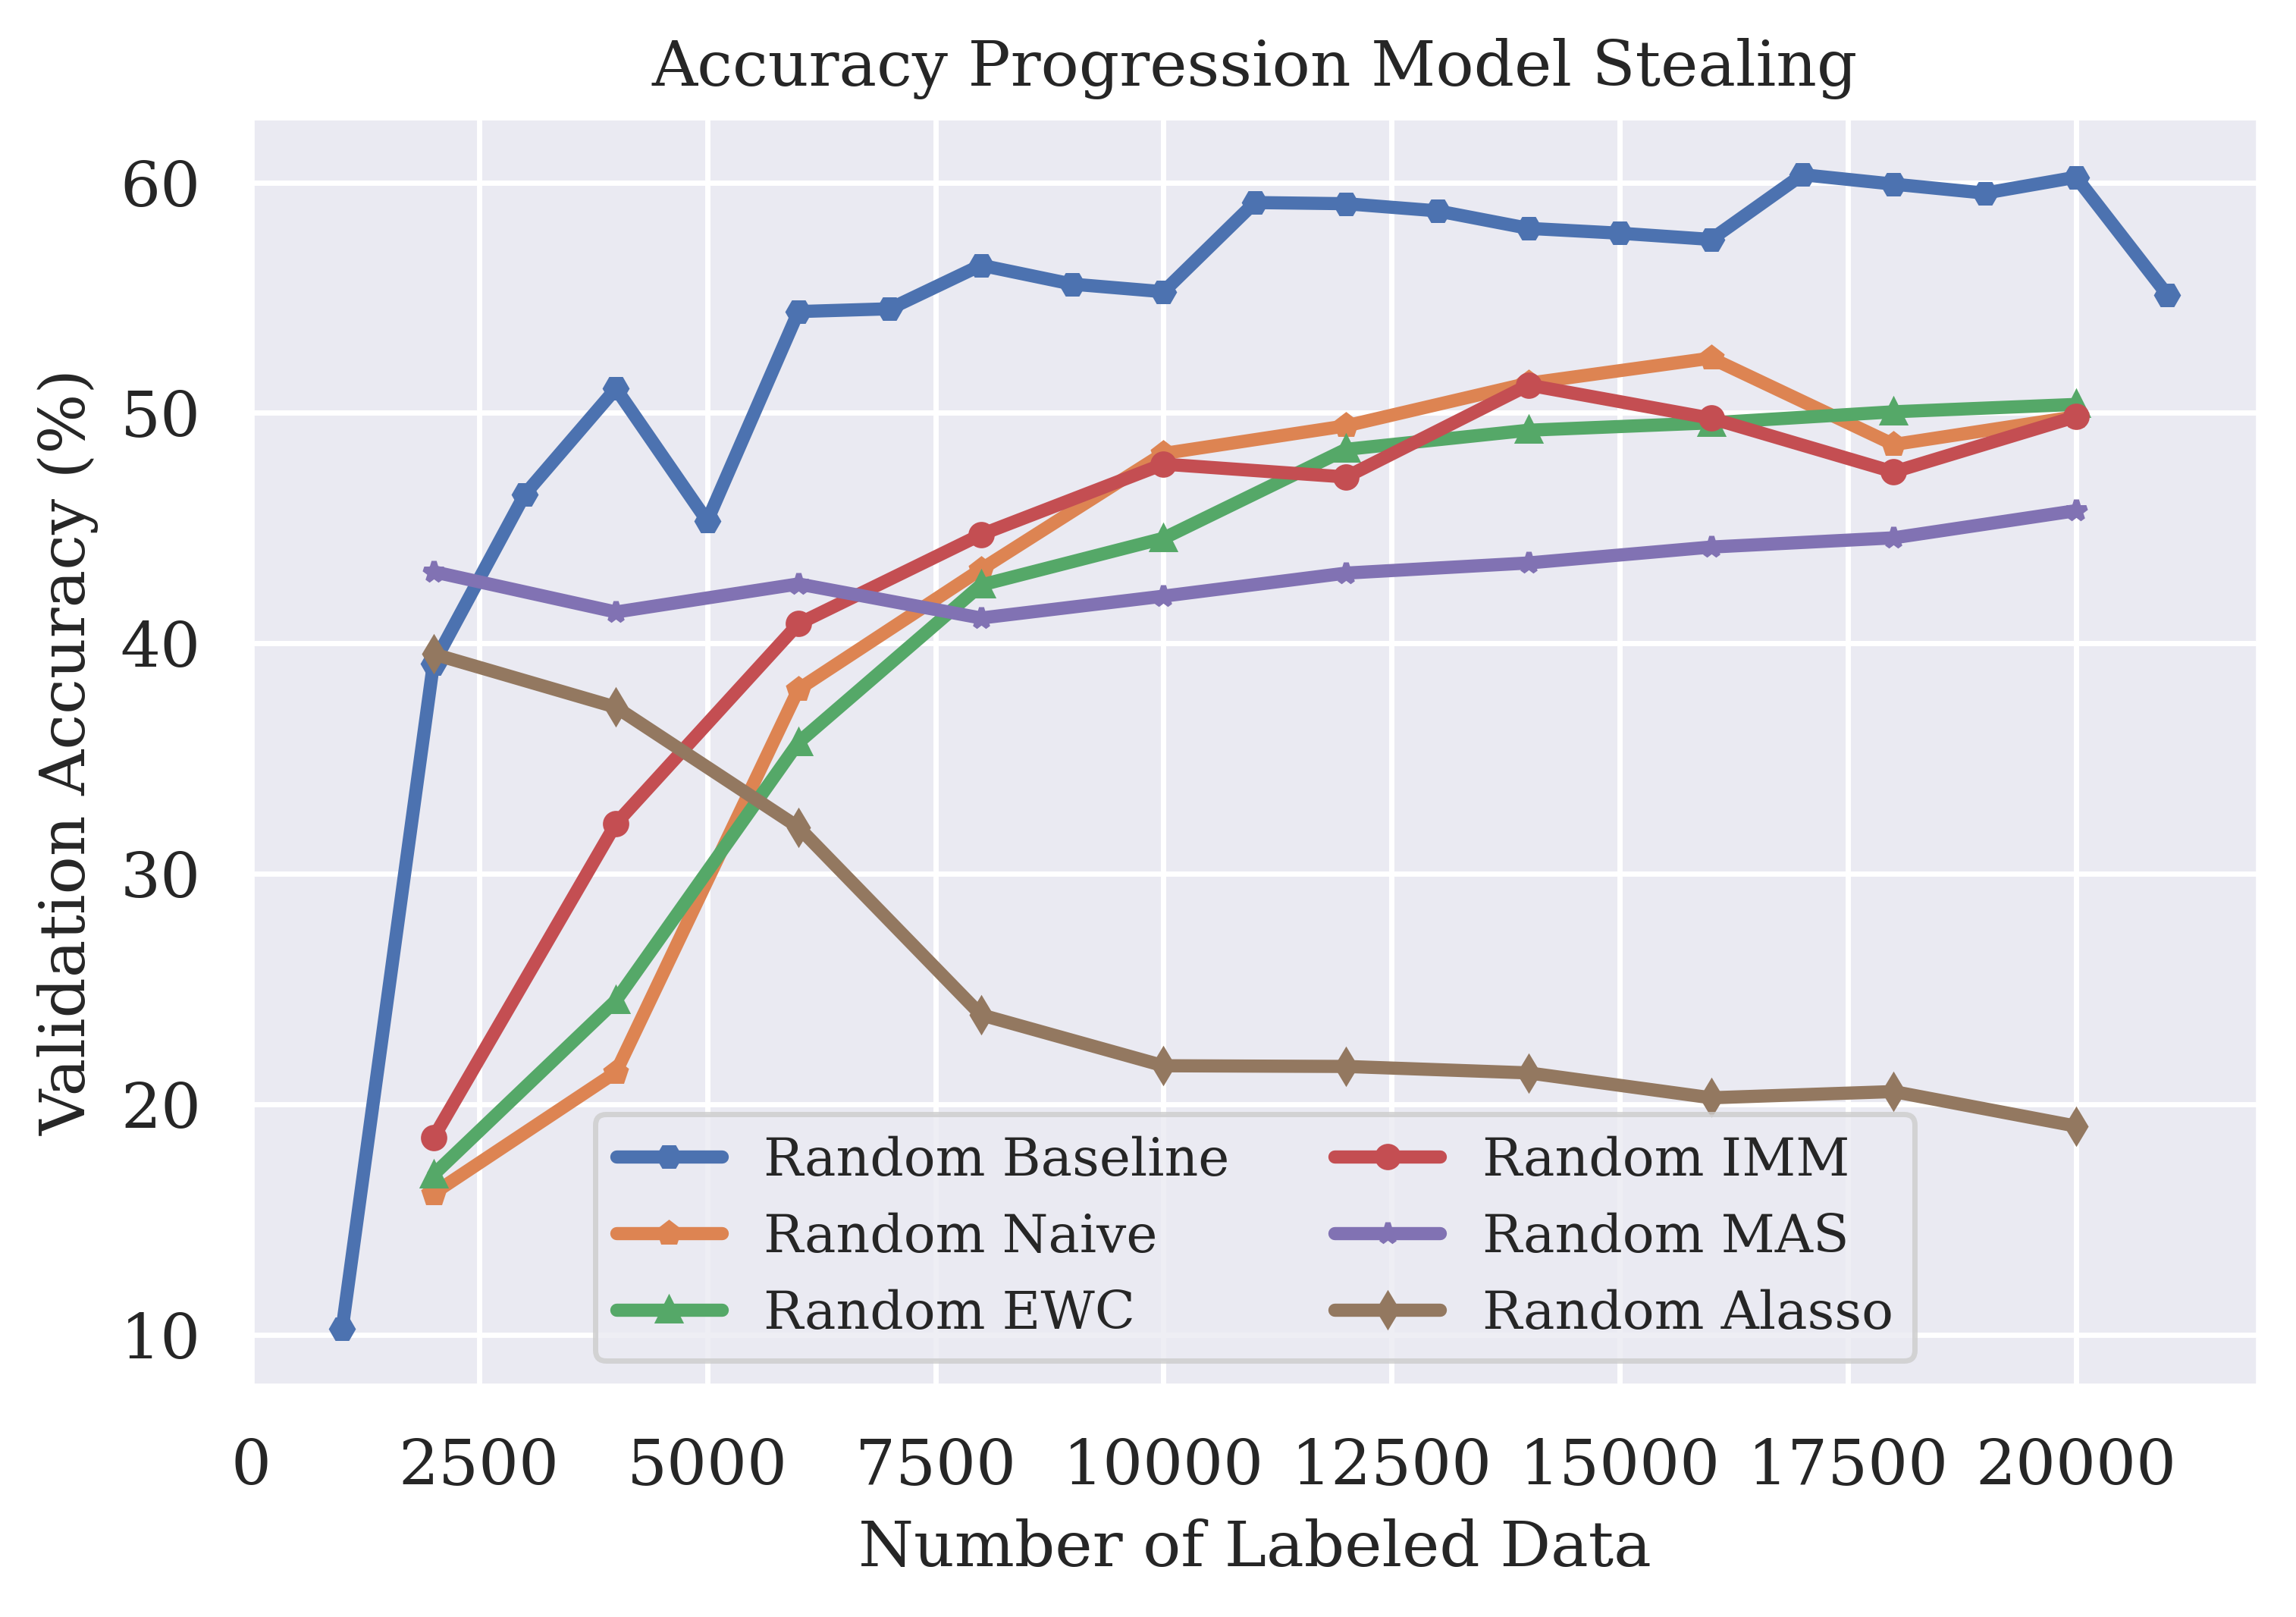
\includegraphics[width=0.7\linewidth]{images/results_CALMS/cifar_label_random.png}
    \caption[Agreement Comparison for Model Stealing on CIFAR10 using the predicted class label and the Active Learning strategy Random]{Progression of Model Agreement
    (in \%) for Model Stealing Attacks using Continual Active Learning on the MNIST dataset. We use Model Stealing Attacks with random sampling
    and train using the predicted class label of the Target Model.}
    \label{fig:CALMSCIFAR10LabelRandom}
\end{figure}

\begin{figure}[h]
    \centering
    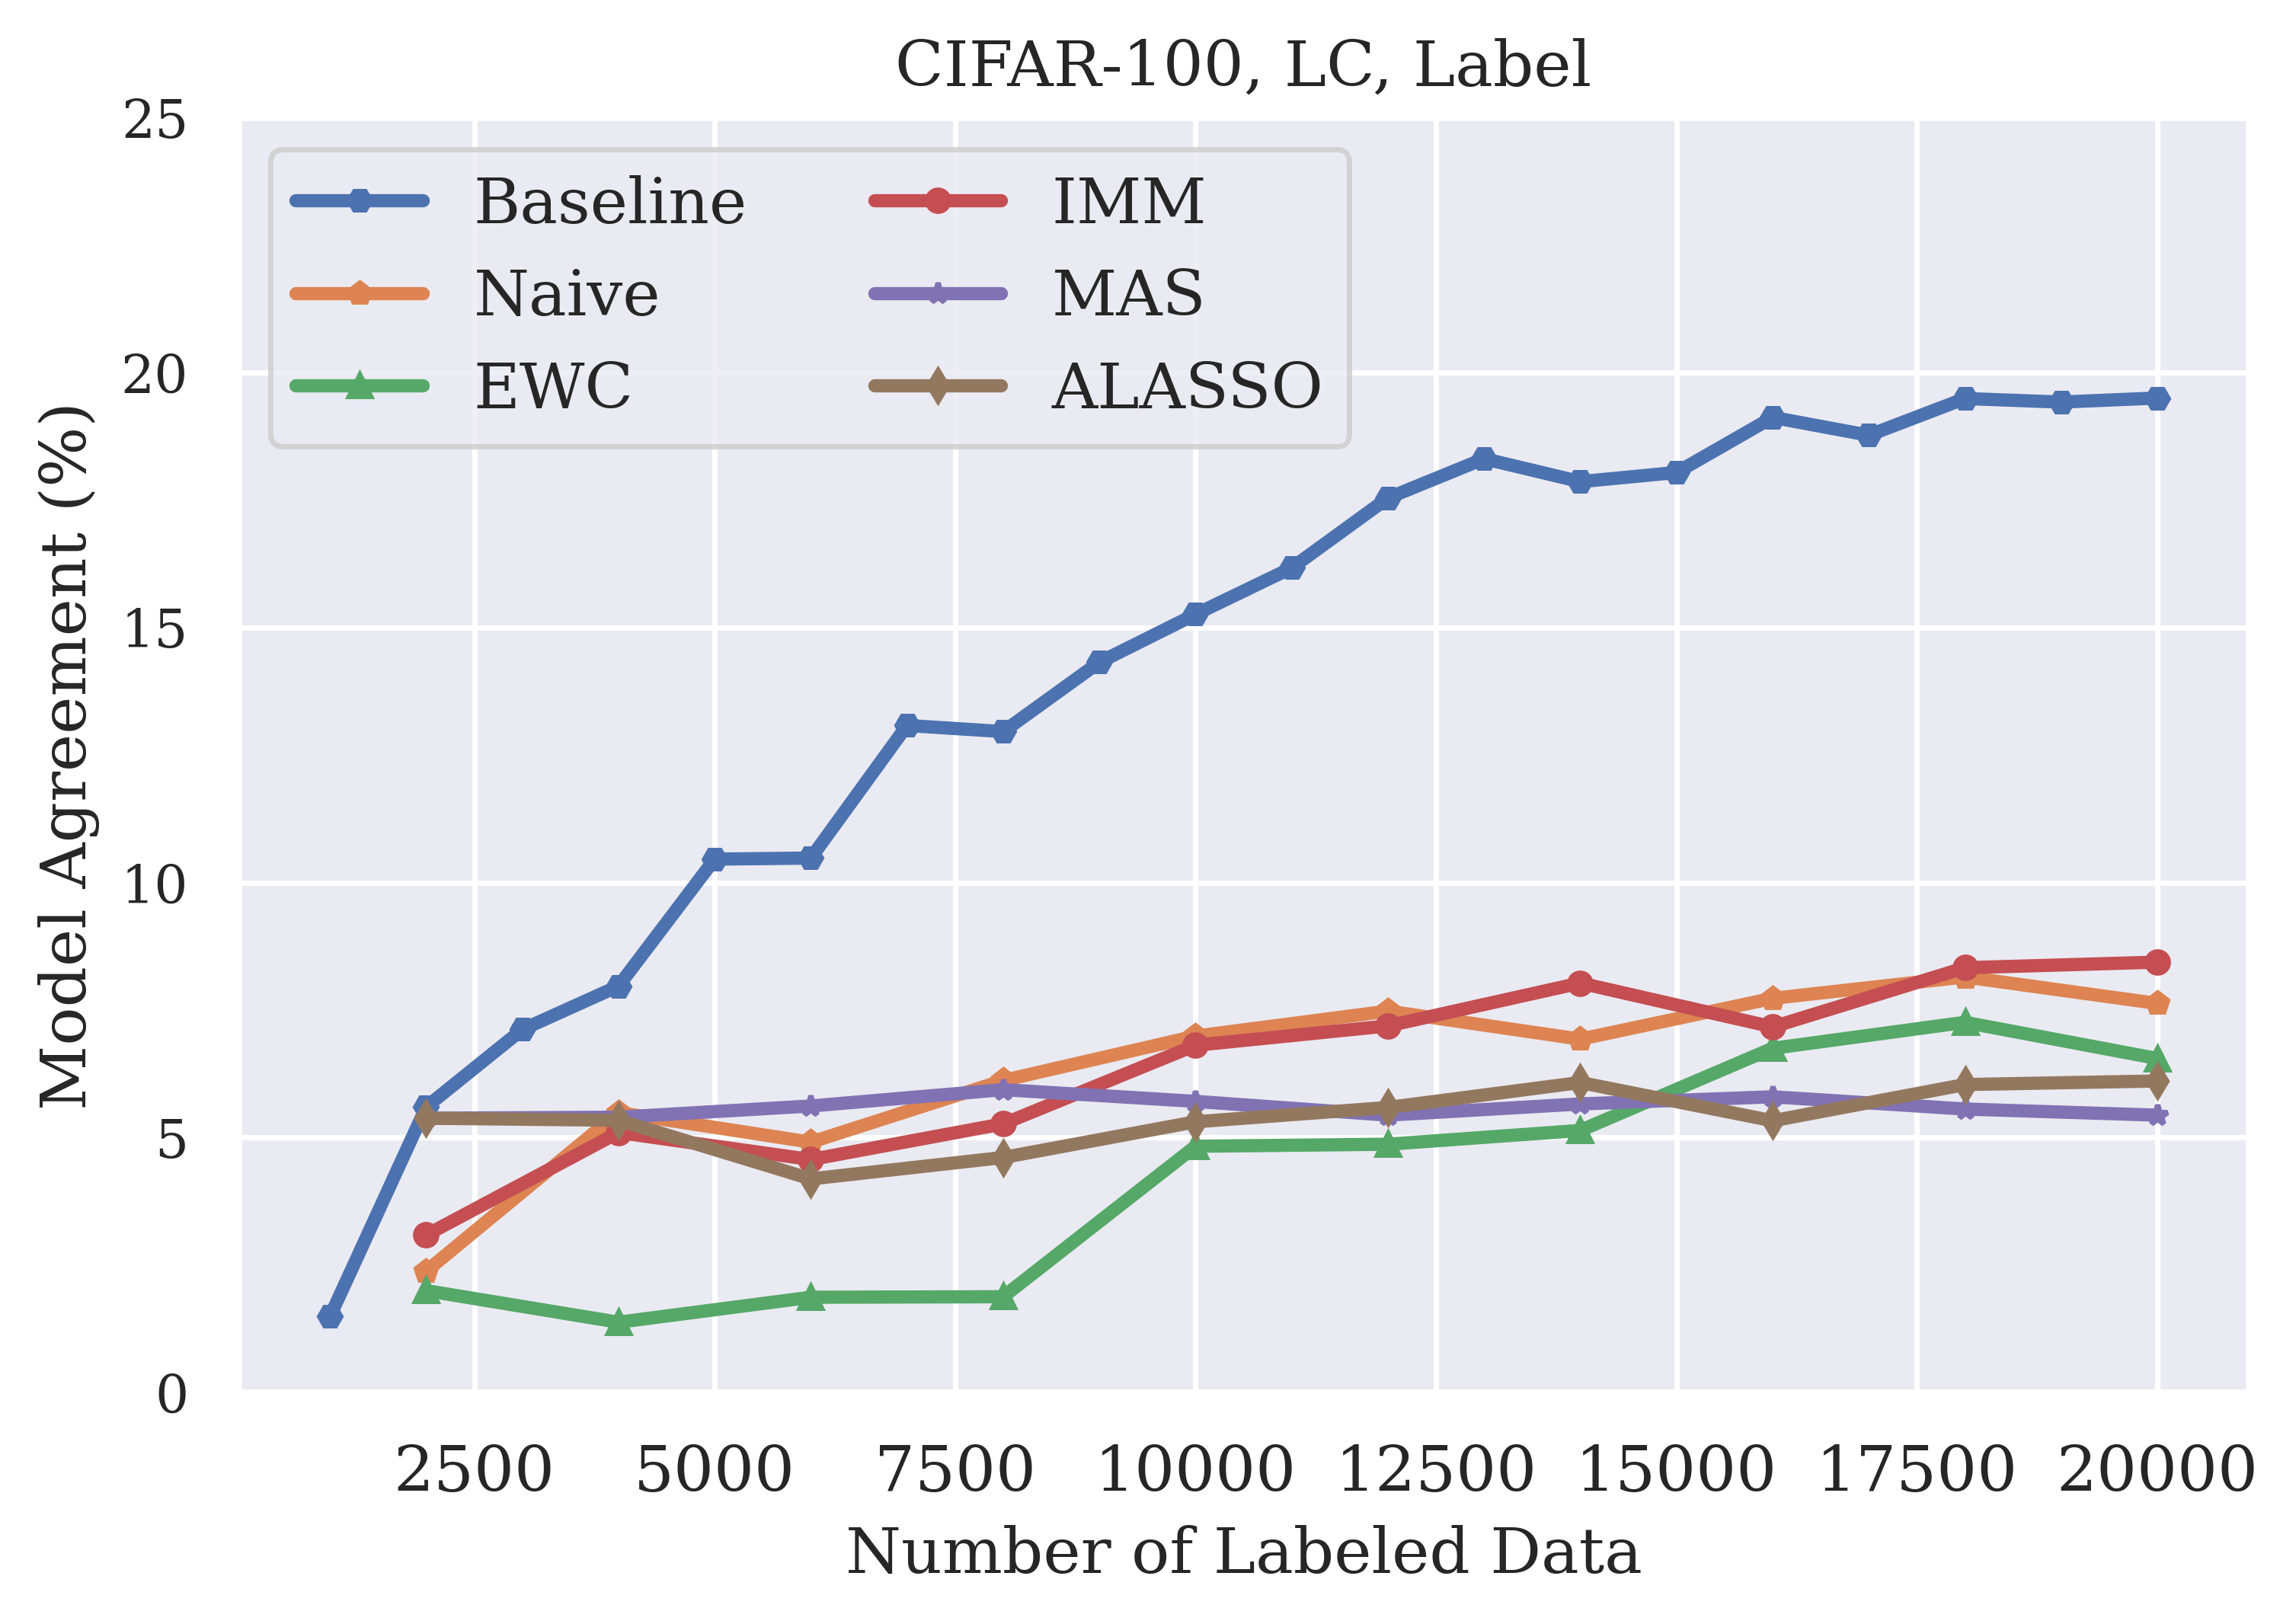
\includegraphics[width=0.7\linewidth]{images/results_CALMS/cifar100_label_lc.png}
    \caption[Agreement Comparison for Model Stealing on CIFAR10 using the predicted class label and the Active Learning strategy LC]{Progression of Model Agreement
    (in \%) for Model Stealing Attacks using Continual Active Learning on the MNIST dataset. We use Model Stealing Attacks with the Active Learning strategy
    \gls{lc} and train using the predicted class label of the Target Model.}
    \label{fig:CALMSCIFAR10LabelLC}
\end{figure}

\begin{figure}[h]
    \centering
    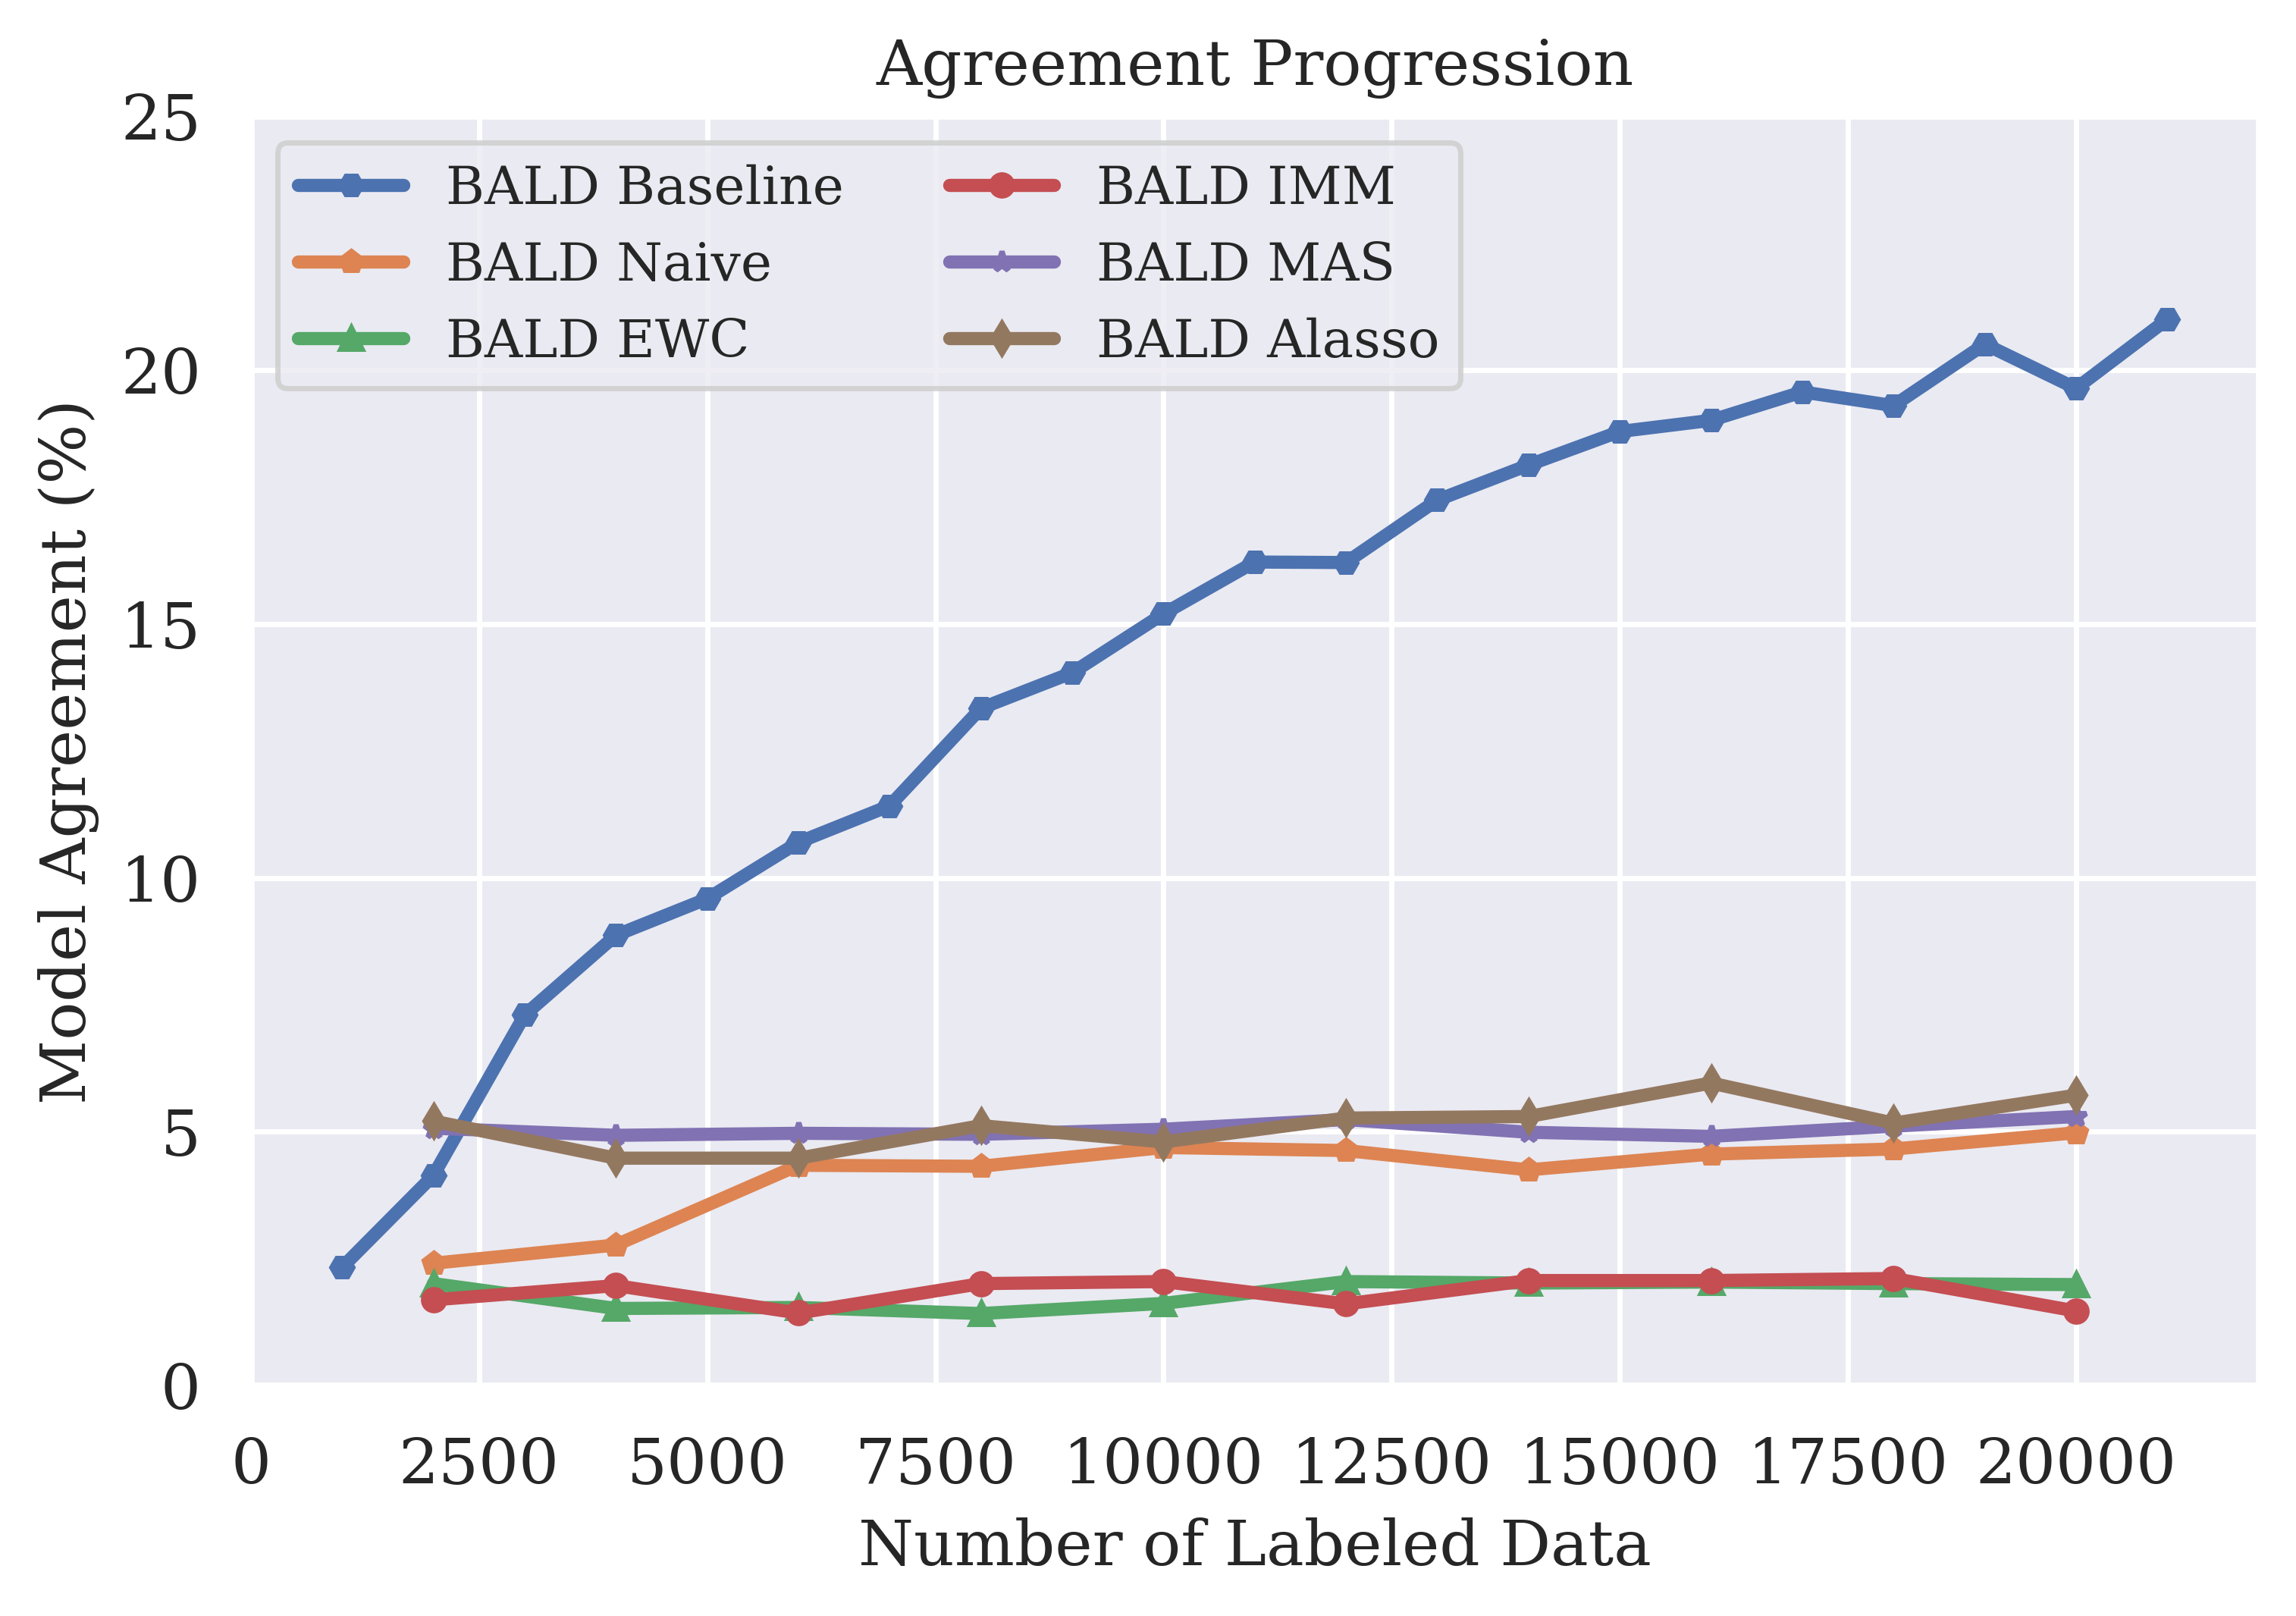
\includegraphics[width=0.7\linewidth]{images/results_CALMS/cifar100_label_bald.png}
    \caption[Agreement Comparison for Model Stealing on CIFAR10 using the predicted class label and the Active Learning strategy BALD]{Progression of Model Agreement
    (in \%) for Model Stealing Attacks using Continual Active Learning on the MNIST dataset. We use Model Stealing Attacks with the Active Learning strategy
    \gls{bald} and train using the predicted class label of the Target Model.}
    \label{fig:CALMSCIFAR10LabelBALD}
\end{figure}

\begin{figure}[h]
    \centering
    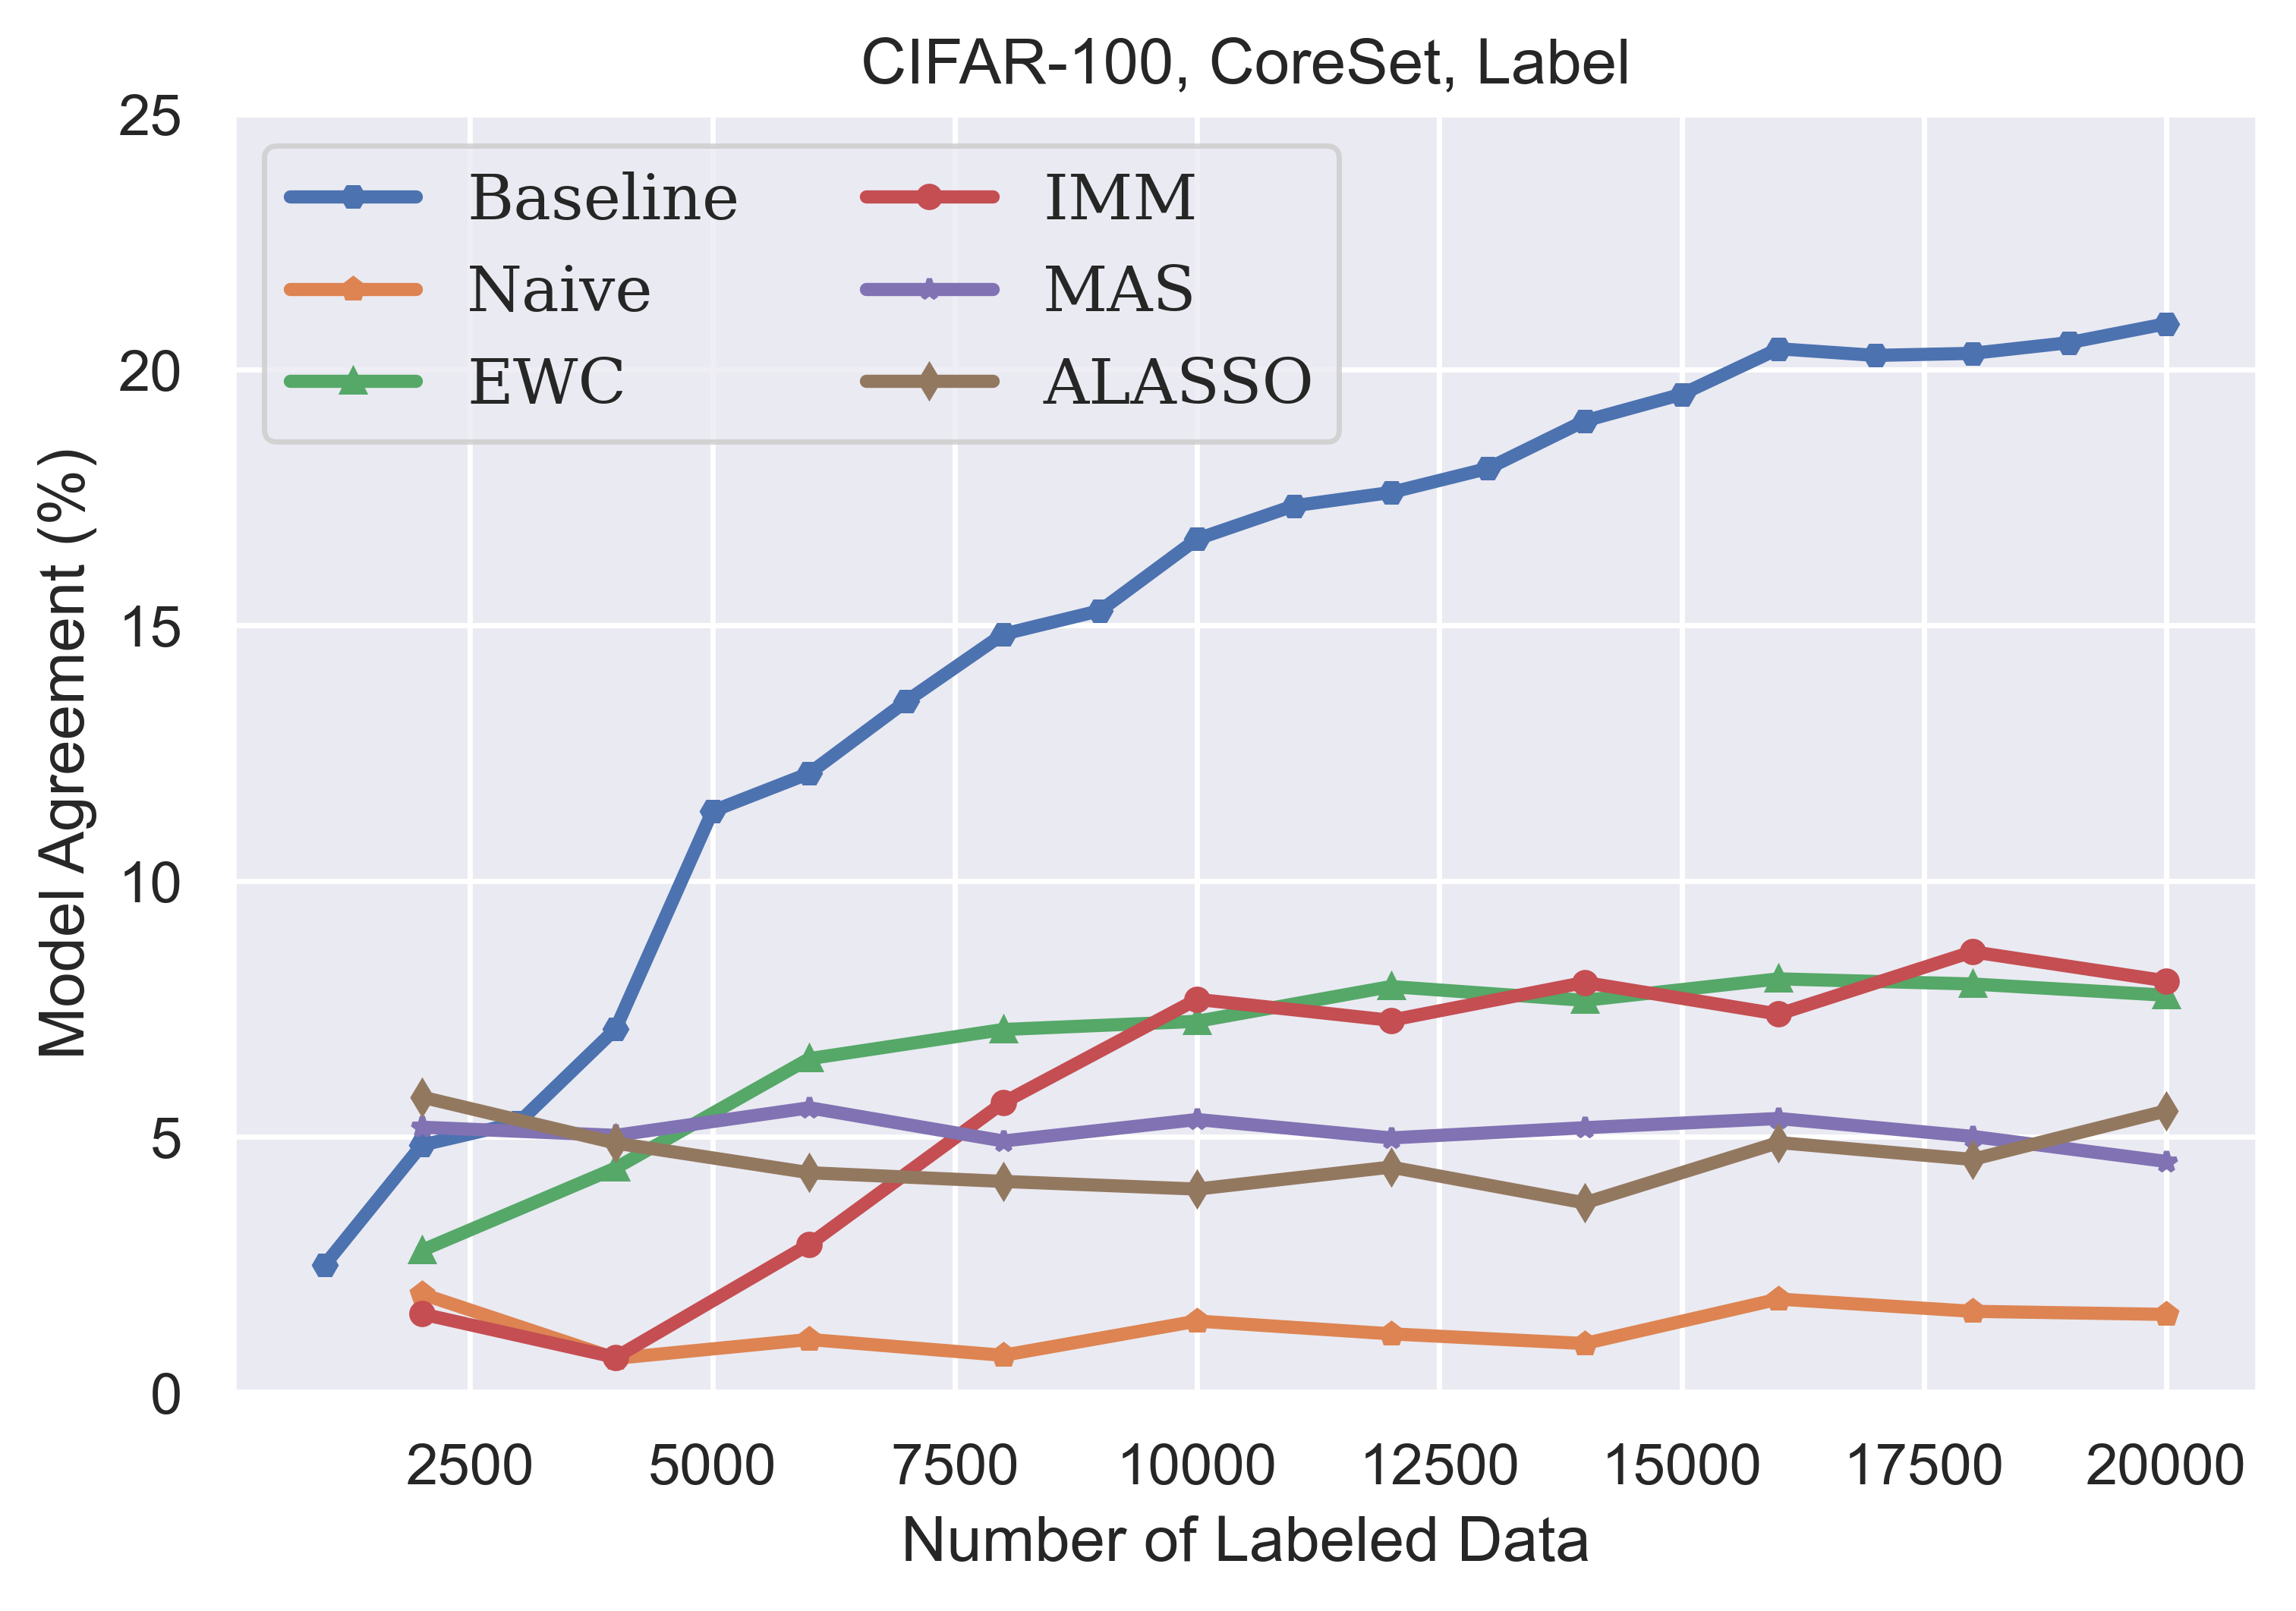
\includegraphics[width=0.7\linewidth]{images/results_CALMS/cifar100_label_coreset.png}
    \caption[Agreement Comparison for Model Stealing on CIFAR10 using the predicted class label and the Active Learning strategy CoreSet]{Progression of Model Agreement
    (in \%) for Model Stealing Attacks using Continual Active Learning on the MNIST dataset. We use Model Stealing Attacks with the Active Learning strategy
    CoreSet and train using the predicted class label of the Target Model.}
    \label{fig:CALMSCIFAR10LabelCoreSet}
\end{figure}

\begin{figure}[h]
    \centering
    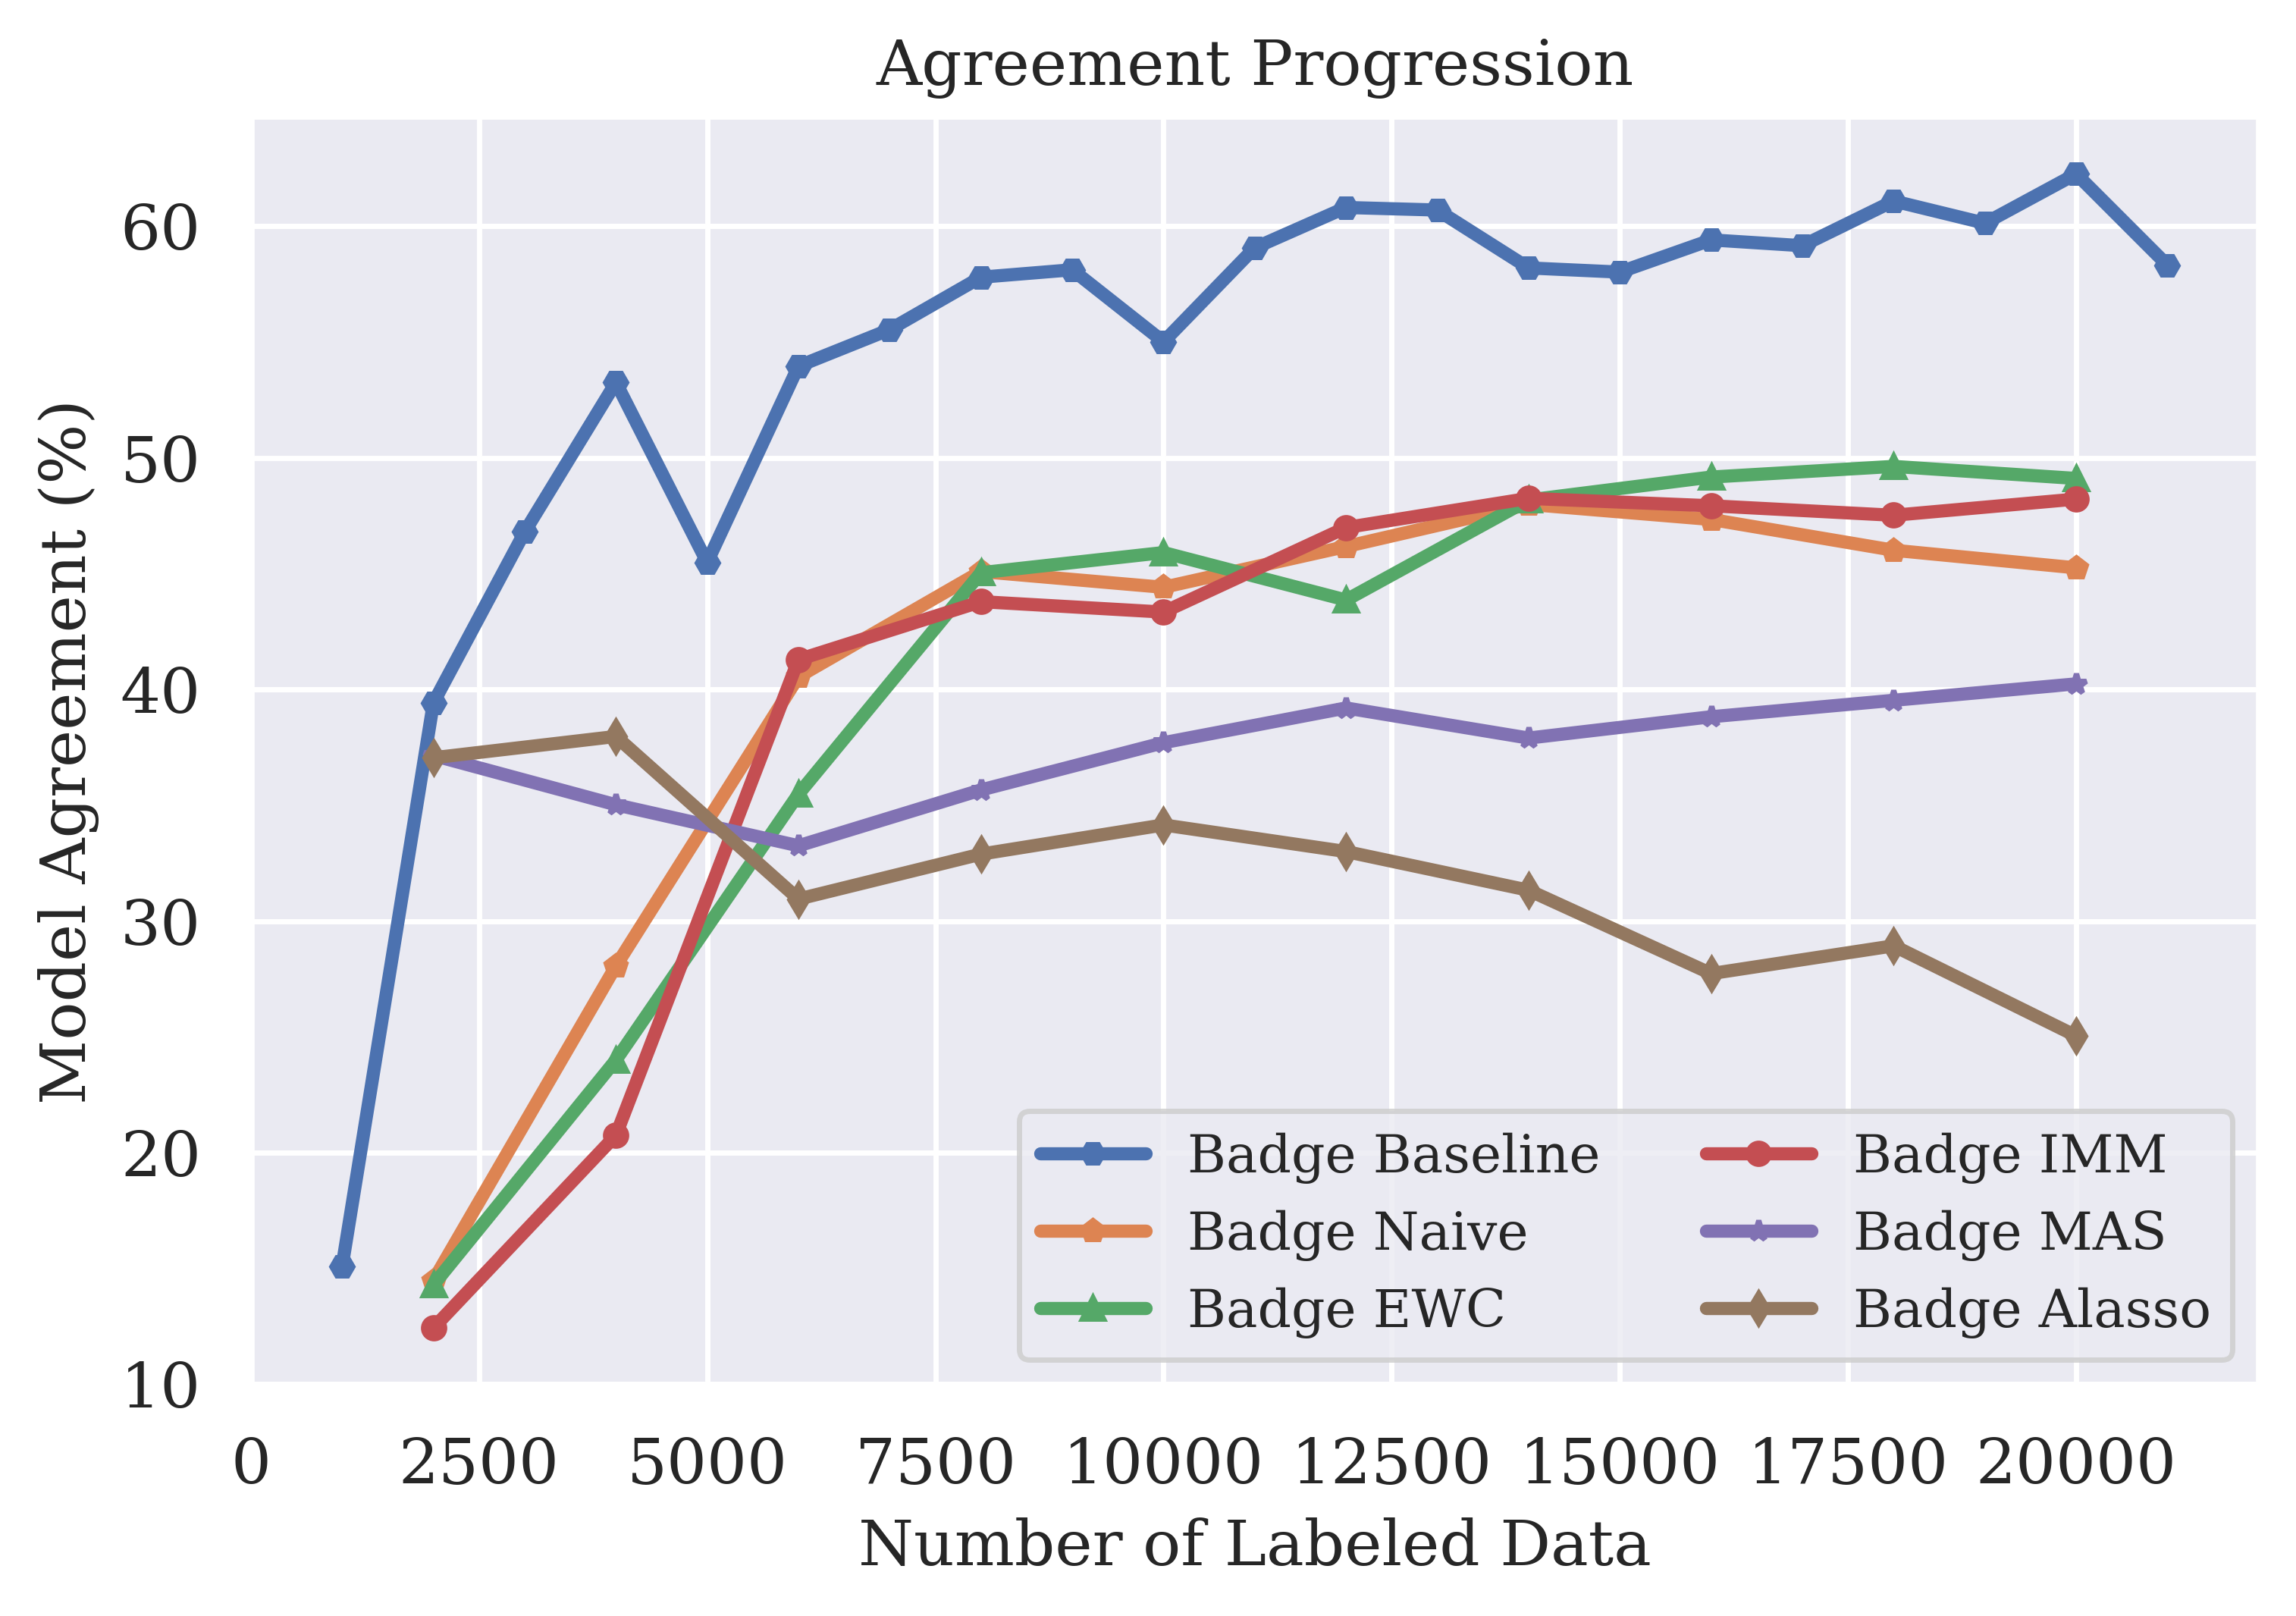
\includegraphics[width=0.7\linewidth]{images/results_CALMS/cifar_label_badge.png}
    \caption[Agreement Comparison for Model Stealing on CIFAR10 using the predicted class label and the Active Learning strategy Badge]{Progression of Model Agreement
    (in \%) for Model Stealing Attacks using Continual Active Learning on the MNIST dataset. We use Model Stealing Attacks with the Active Learning strategy
    \gls{badge} and train using the predicted class label of the Target Model.}
    \label{fig:CALMSCIFAR10LabelBadge}
\end{figure}

%Softmax
\begin{figure}[h]
    \centering
    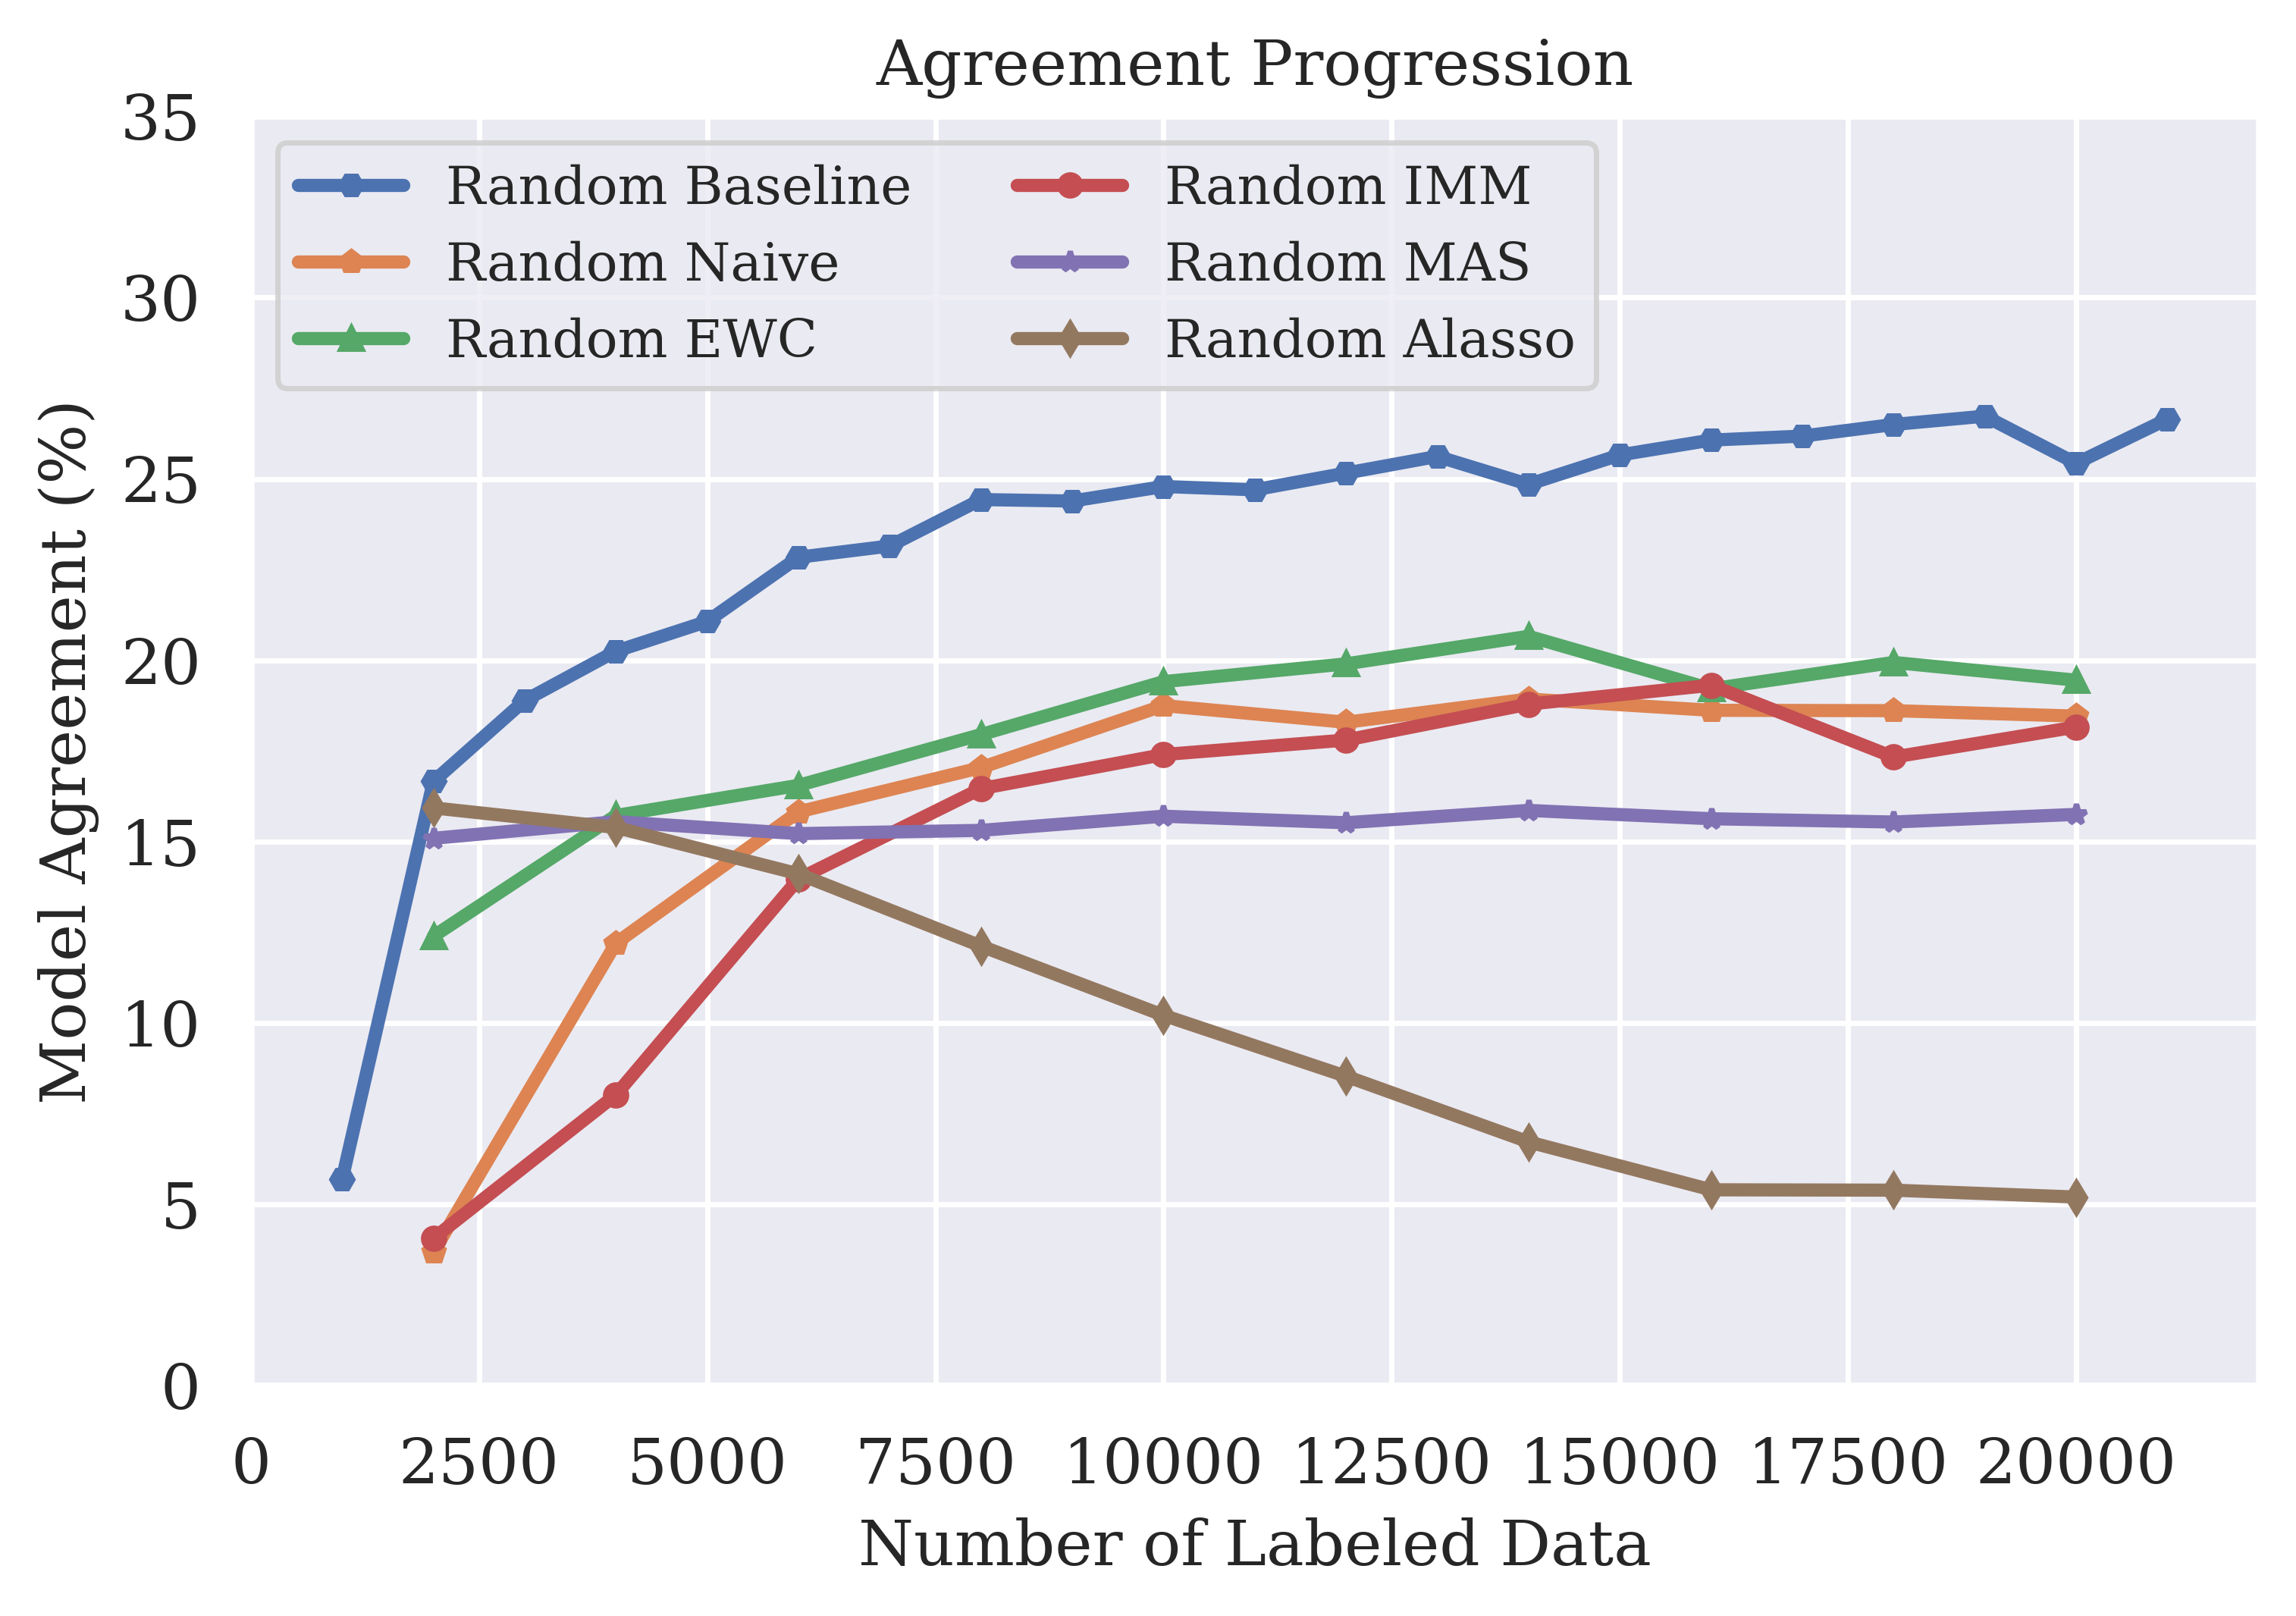
\includegraphics[width=0.7\linewidth]{images/results_CALMS/cifar100_softmax_random.png}
    \caption[Agreement Comparison for Model Stealing on CIFAR10 using the softmax output and the Active Learning strategy Random]{Progression of Model Agreement
    (in \%) for Model Stealing Attacks using Continual Active Learning on the CIFAR-10 dataset. We use Model Stealing Attacks with random sampling and train
    using the softmax output of the Target Model.}
    \label{fig:CALMSCIFAR10SoftmaxRandom}
\end{figure}

\begin{figure}[h]
    \centering
    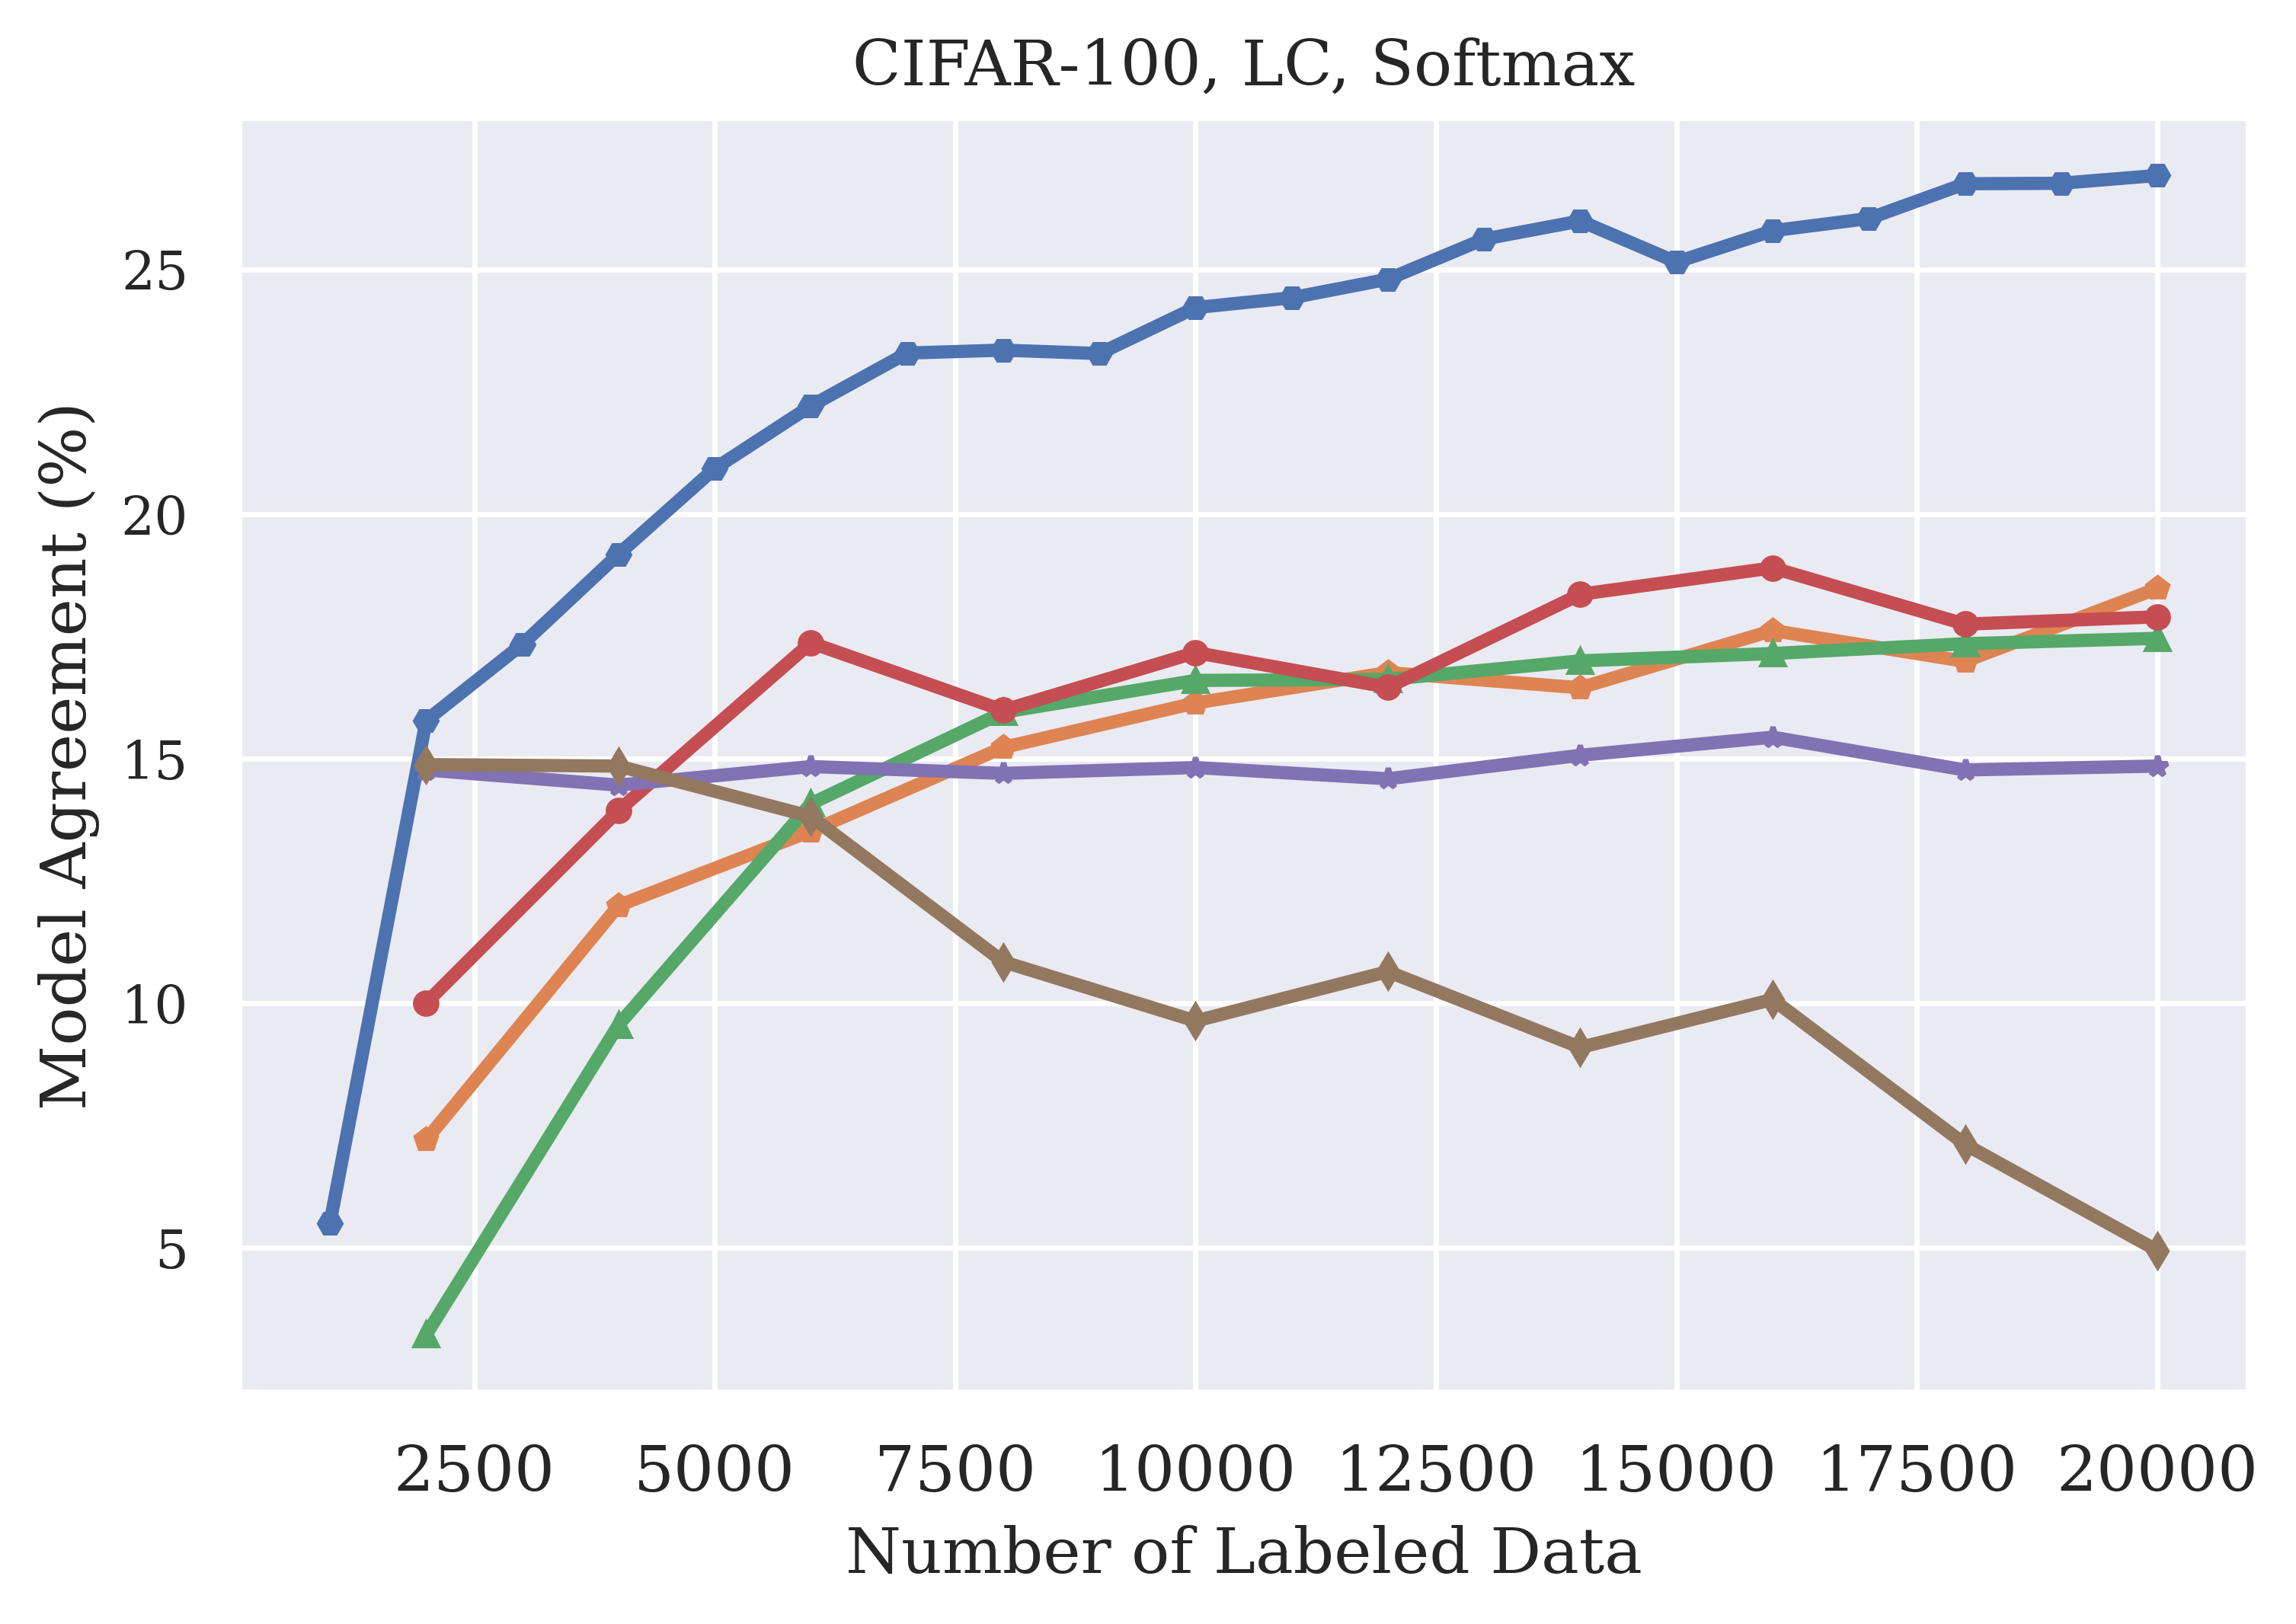
\includegraphics[width=0.7\linewidth]{images/results_CALMS/cifar100_softmax_lc.png}
    \caption[Agreement Comparison for Model Stealing on CIFAR10 using the softmax output and the Active Learning strategy LC]{Progression of Model Agreement
    (in \%) for Model Stealing Attacks using Continual Active Learning on the CIFAR-10 dataset. We use Model Stealing Attacks with the Active Learning strategy
    \gls{lc} and train using the softmax output of the Target Model.}
    \label{fig:CALMSCIFAR10SoftmaxLC}
\end{figure}

\begin{figure}[h]
    \centering
    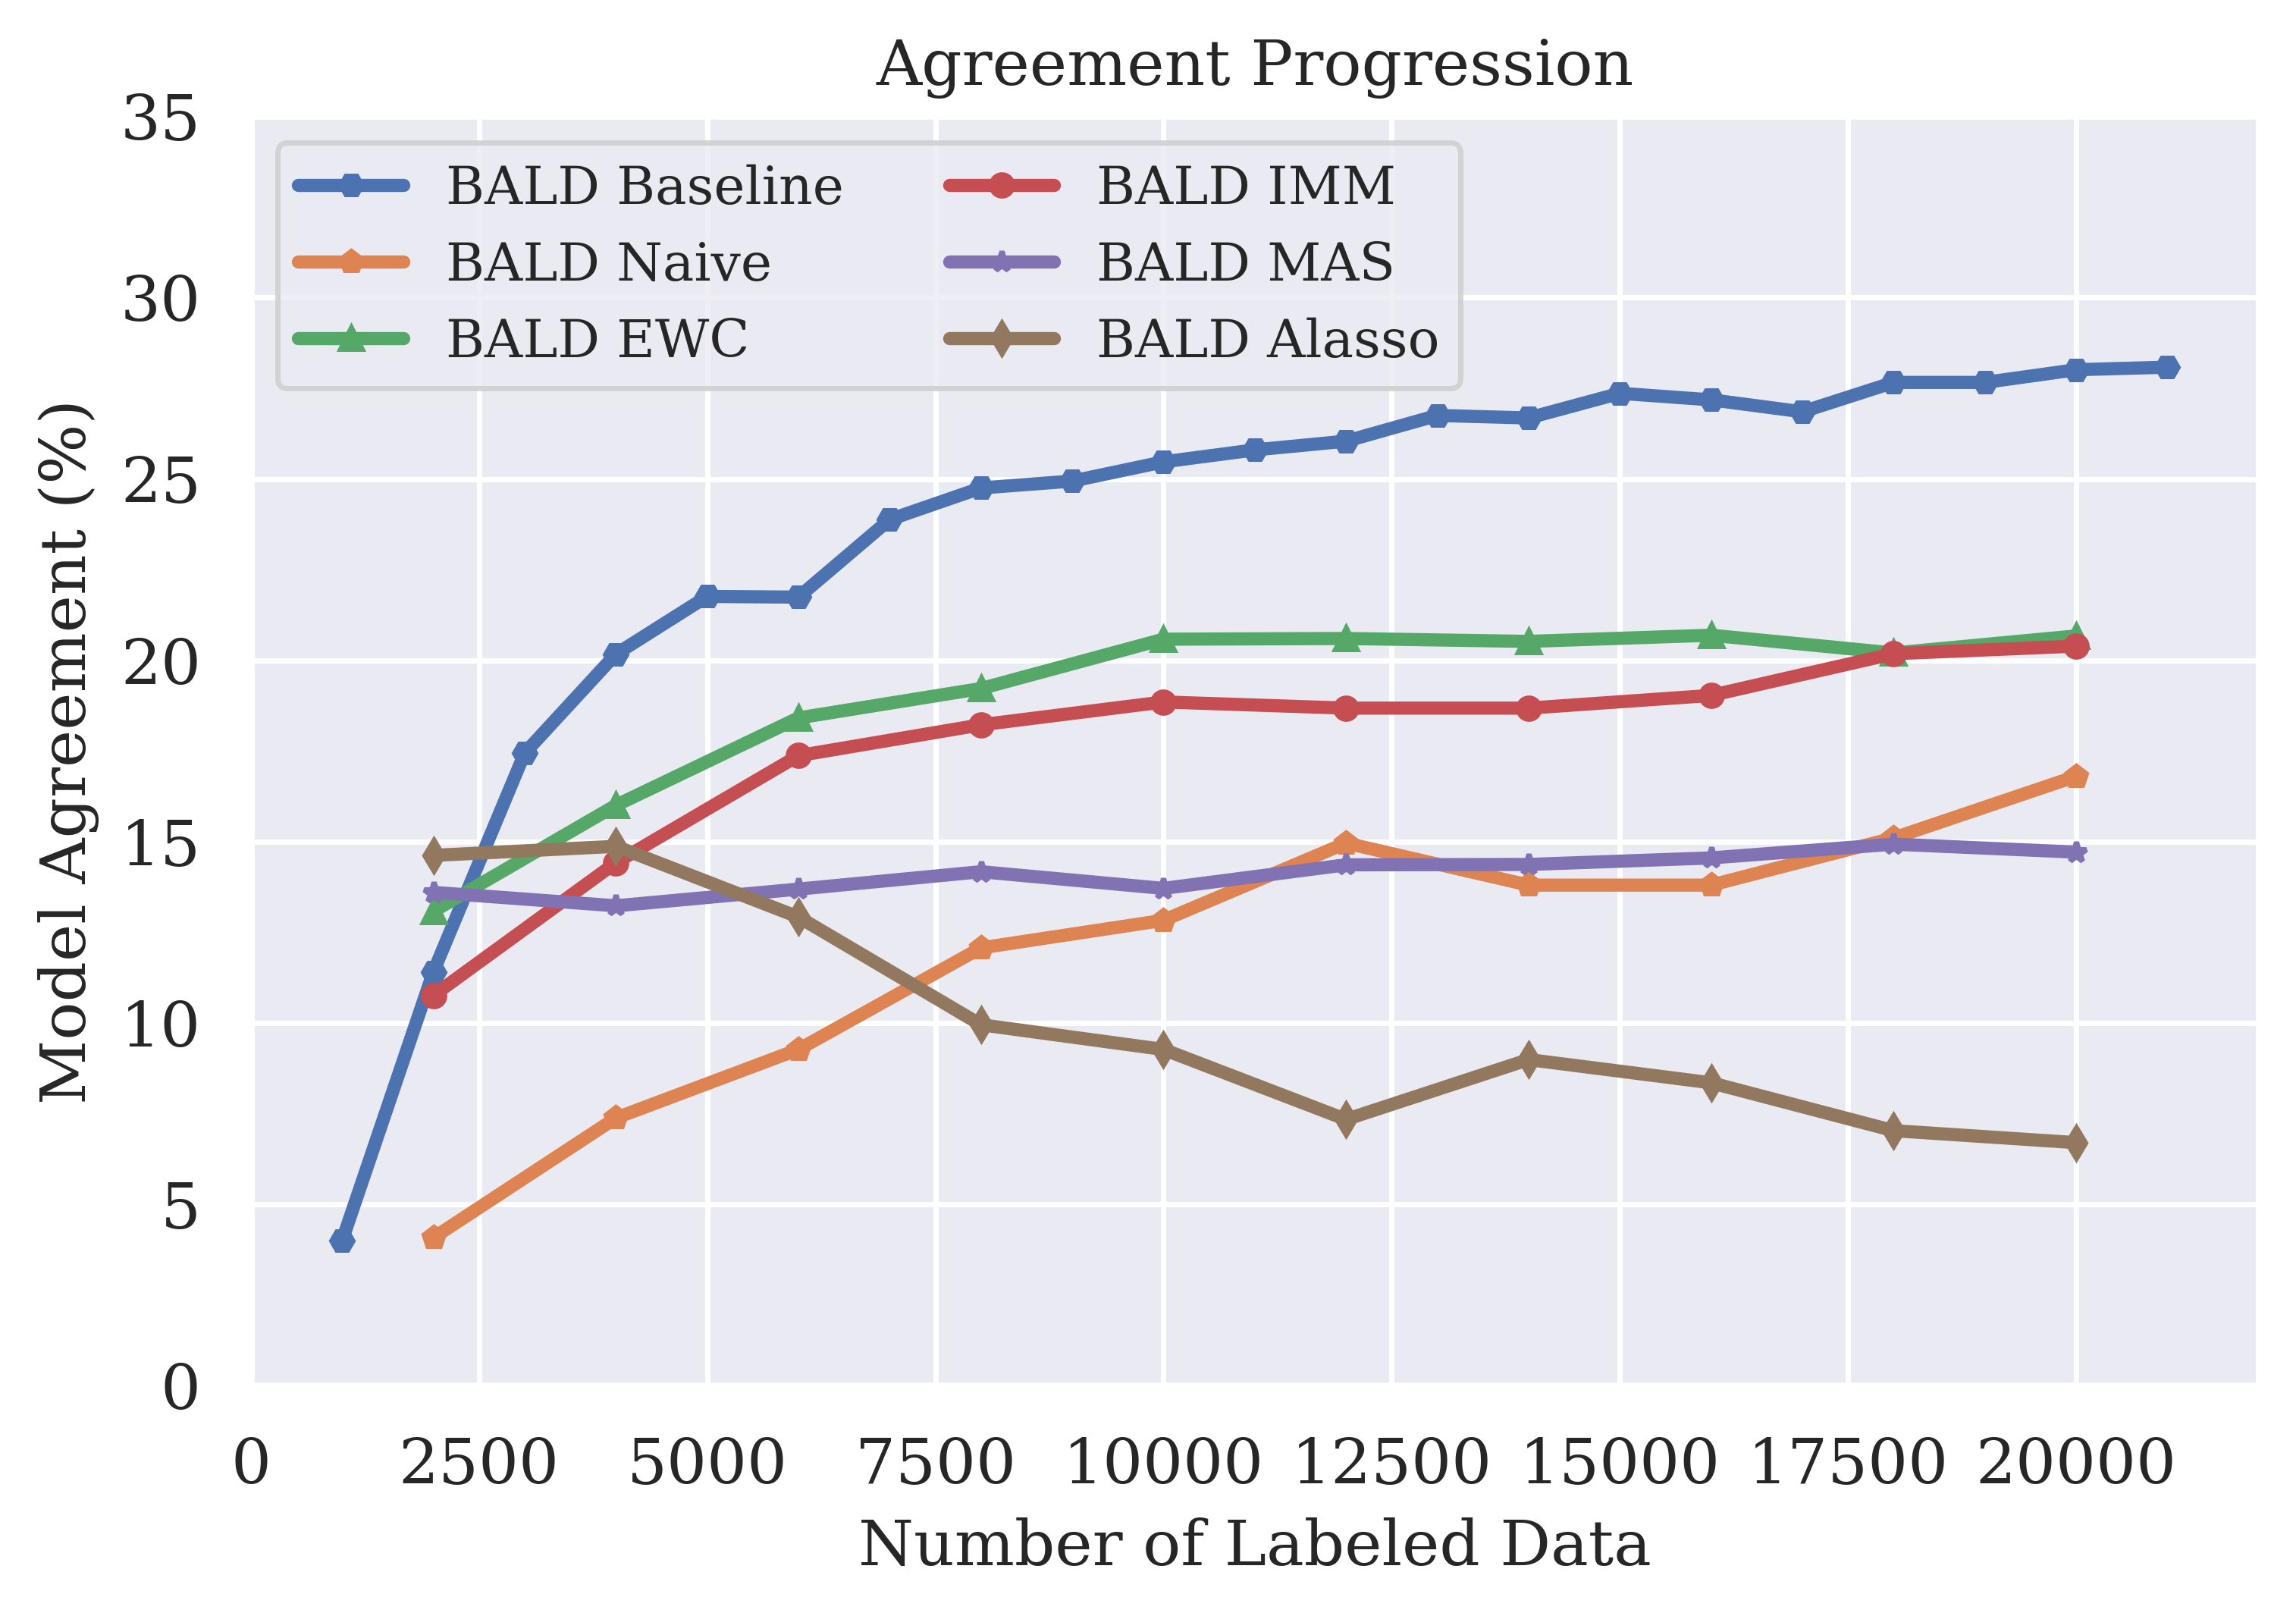
\includegraphics[width=0.7\linewidth]{images/results_CALMS/cifar100_softmax_bald.png}
    \caption[Agreement Comparison for Model Stealing on CIFAR10 using the softmax output and the Active Learning strategy BALD]{Progression of Model Agreement
    (in \%) for Model Stealing Attacks using Continual Active Learning on the CIFAR-10 dataset. We use Model Stealing Attacks with the Active Learning strategy
    \gls{bald} and train using the softmax output of the Target Model.}
    \label{fig:CALMSCIFAR10SoftmaxBALD}
\end{figure}

\begin{figure}[h]
    \centering
    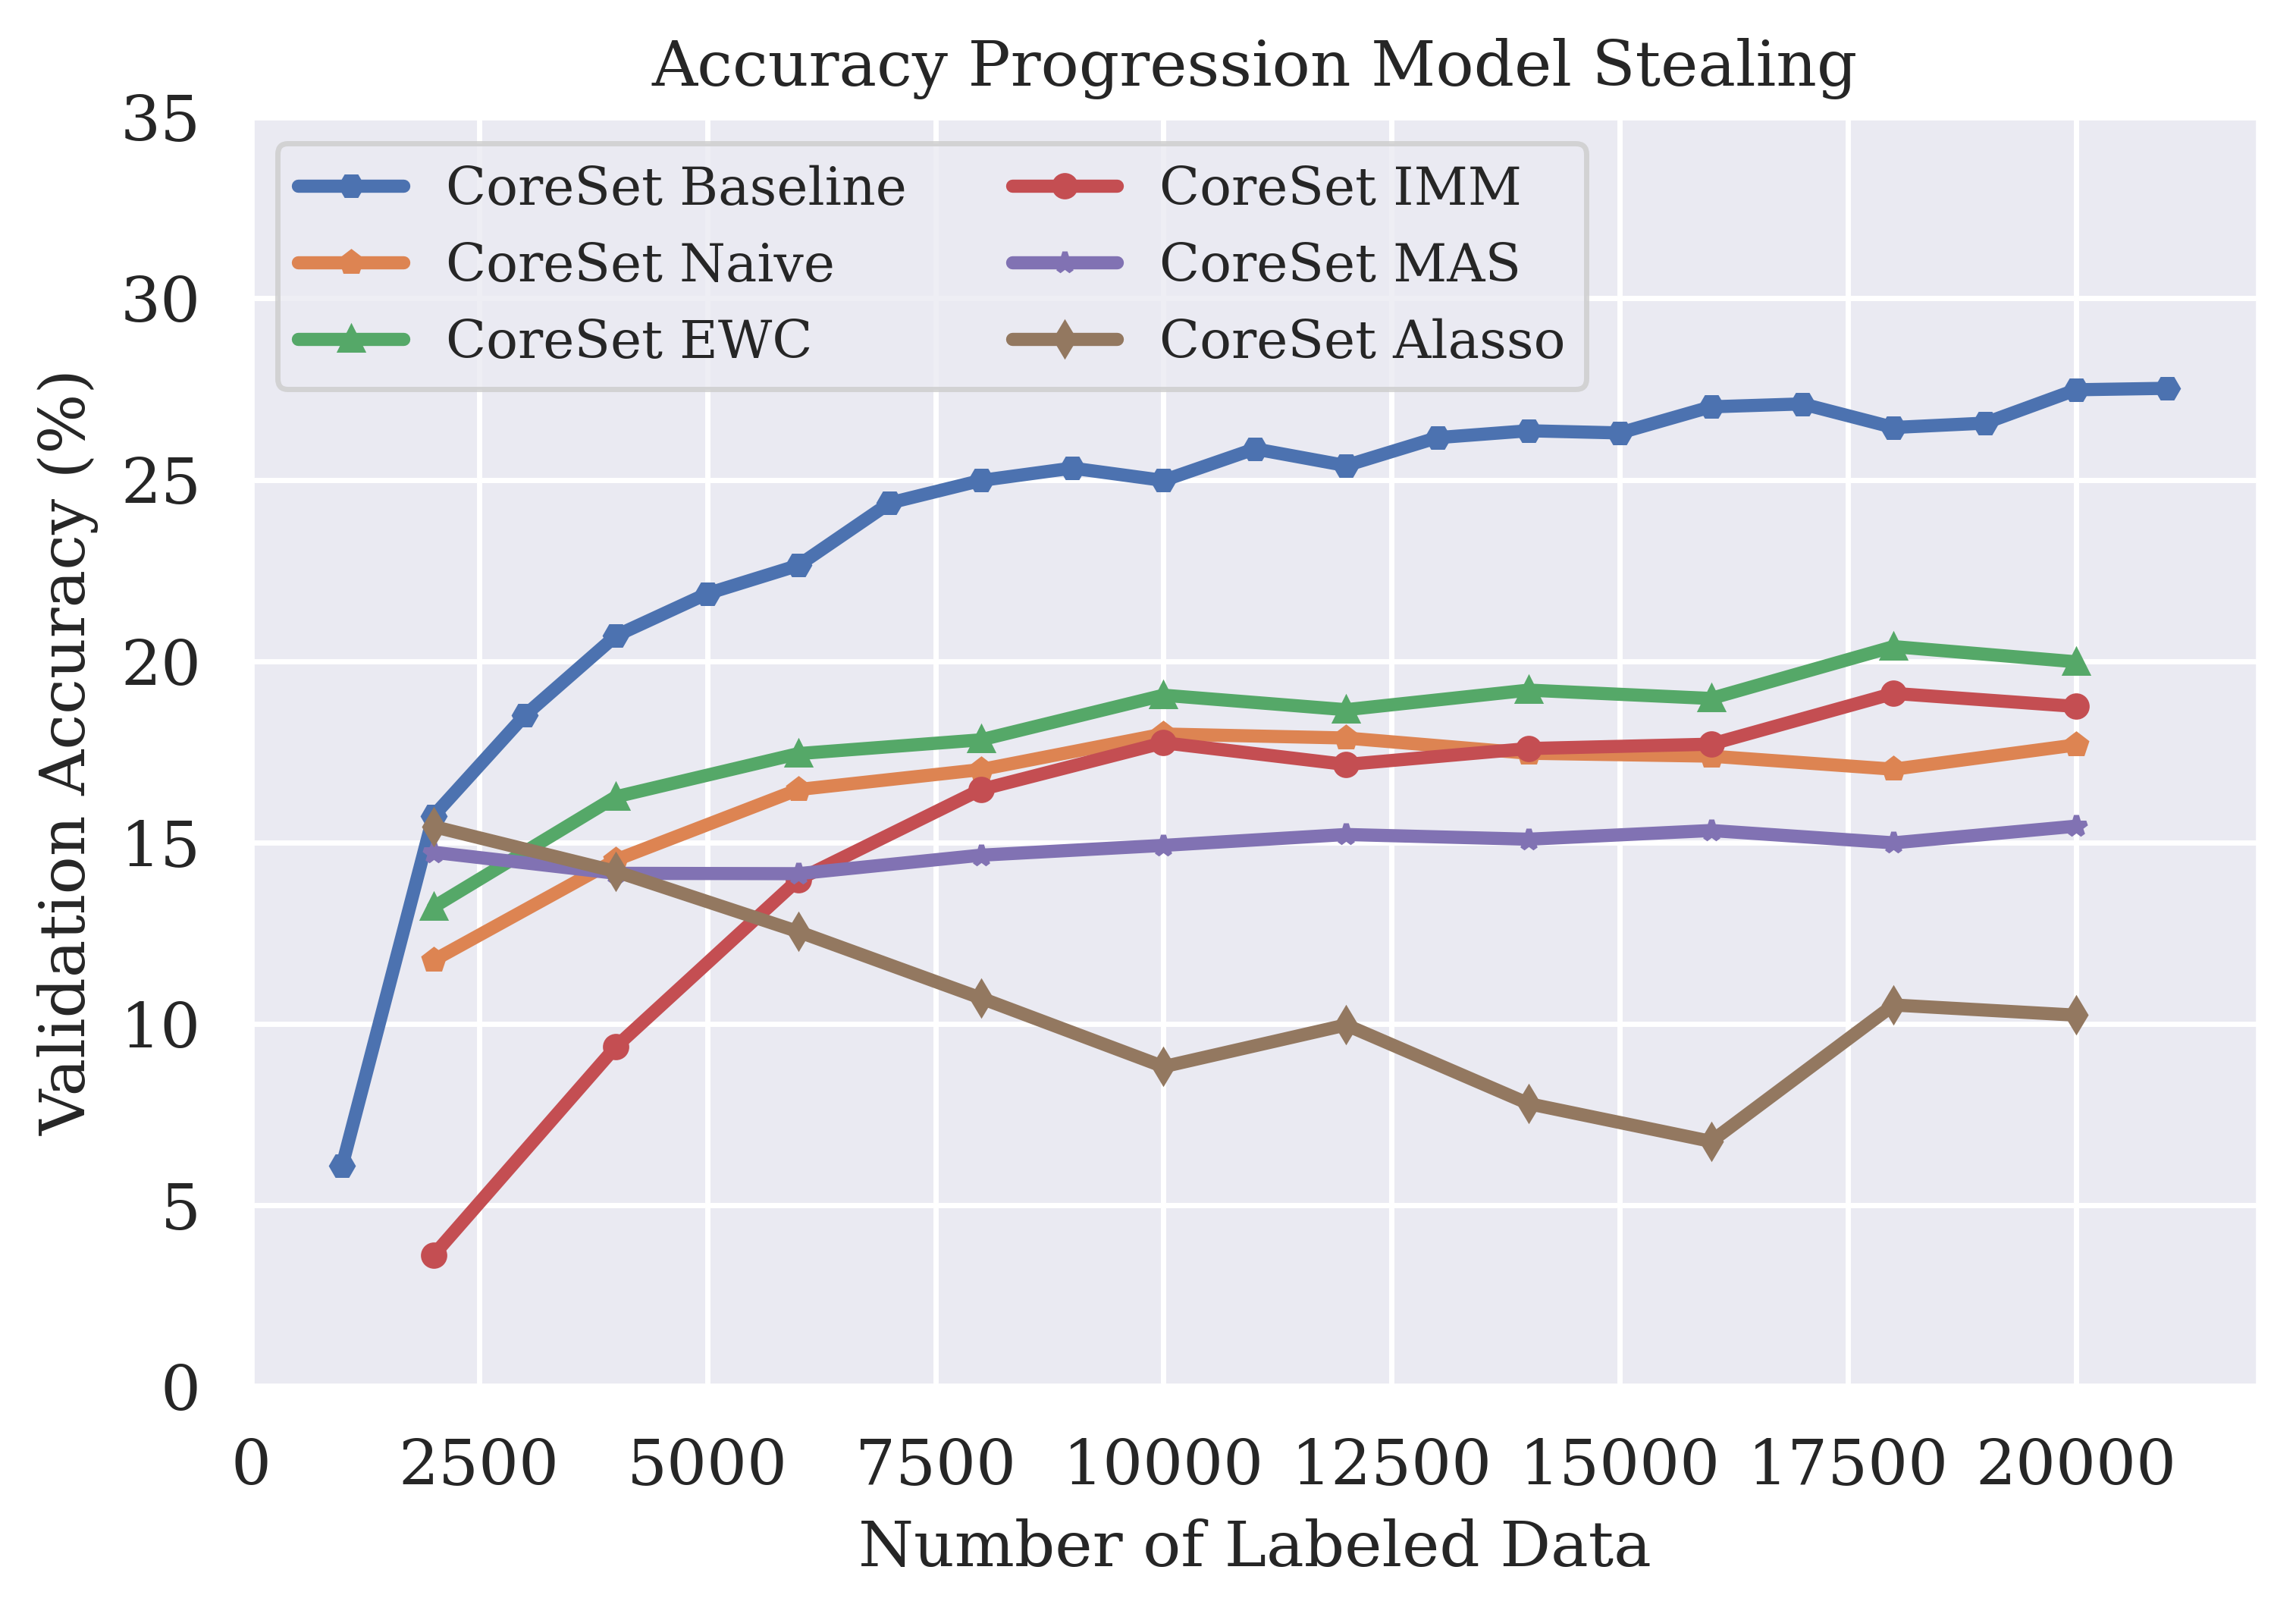
\includegraphics[width=0.7\linewidth]{images/results_CALMS/cifar100_softmax_coreset.png}
    \caption[Agreement Comparison for Model Stealing on CIFAR10 using the softmax output and the Active Learning strategy CoreSet]{Progression of Model Agreement
    (in \%) for Model Stealing Attacks using Continual Active Learning on the CIFAR-10 dataset. We use Model Stealing Attacks with the Active Learning strategy
    CoreSet and train using the softmax output of the Target Model.}
    \label{fig:CALMSCIFAR10SoftmaxCoreSet}
\end{figure}

\begin{figure}[h]
    \centering
    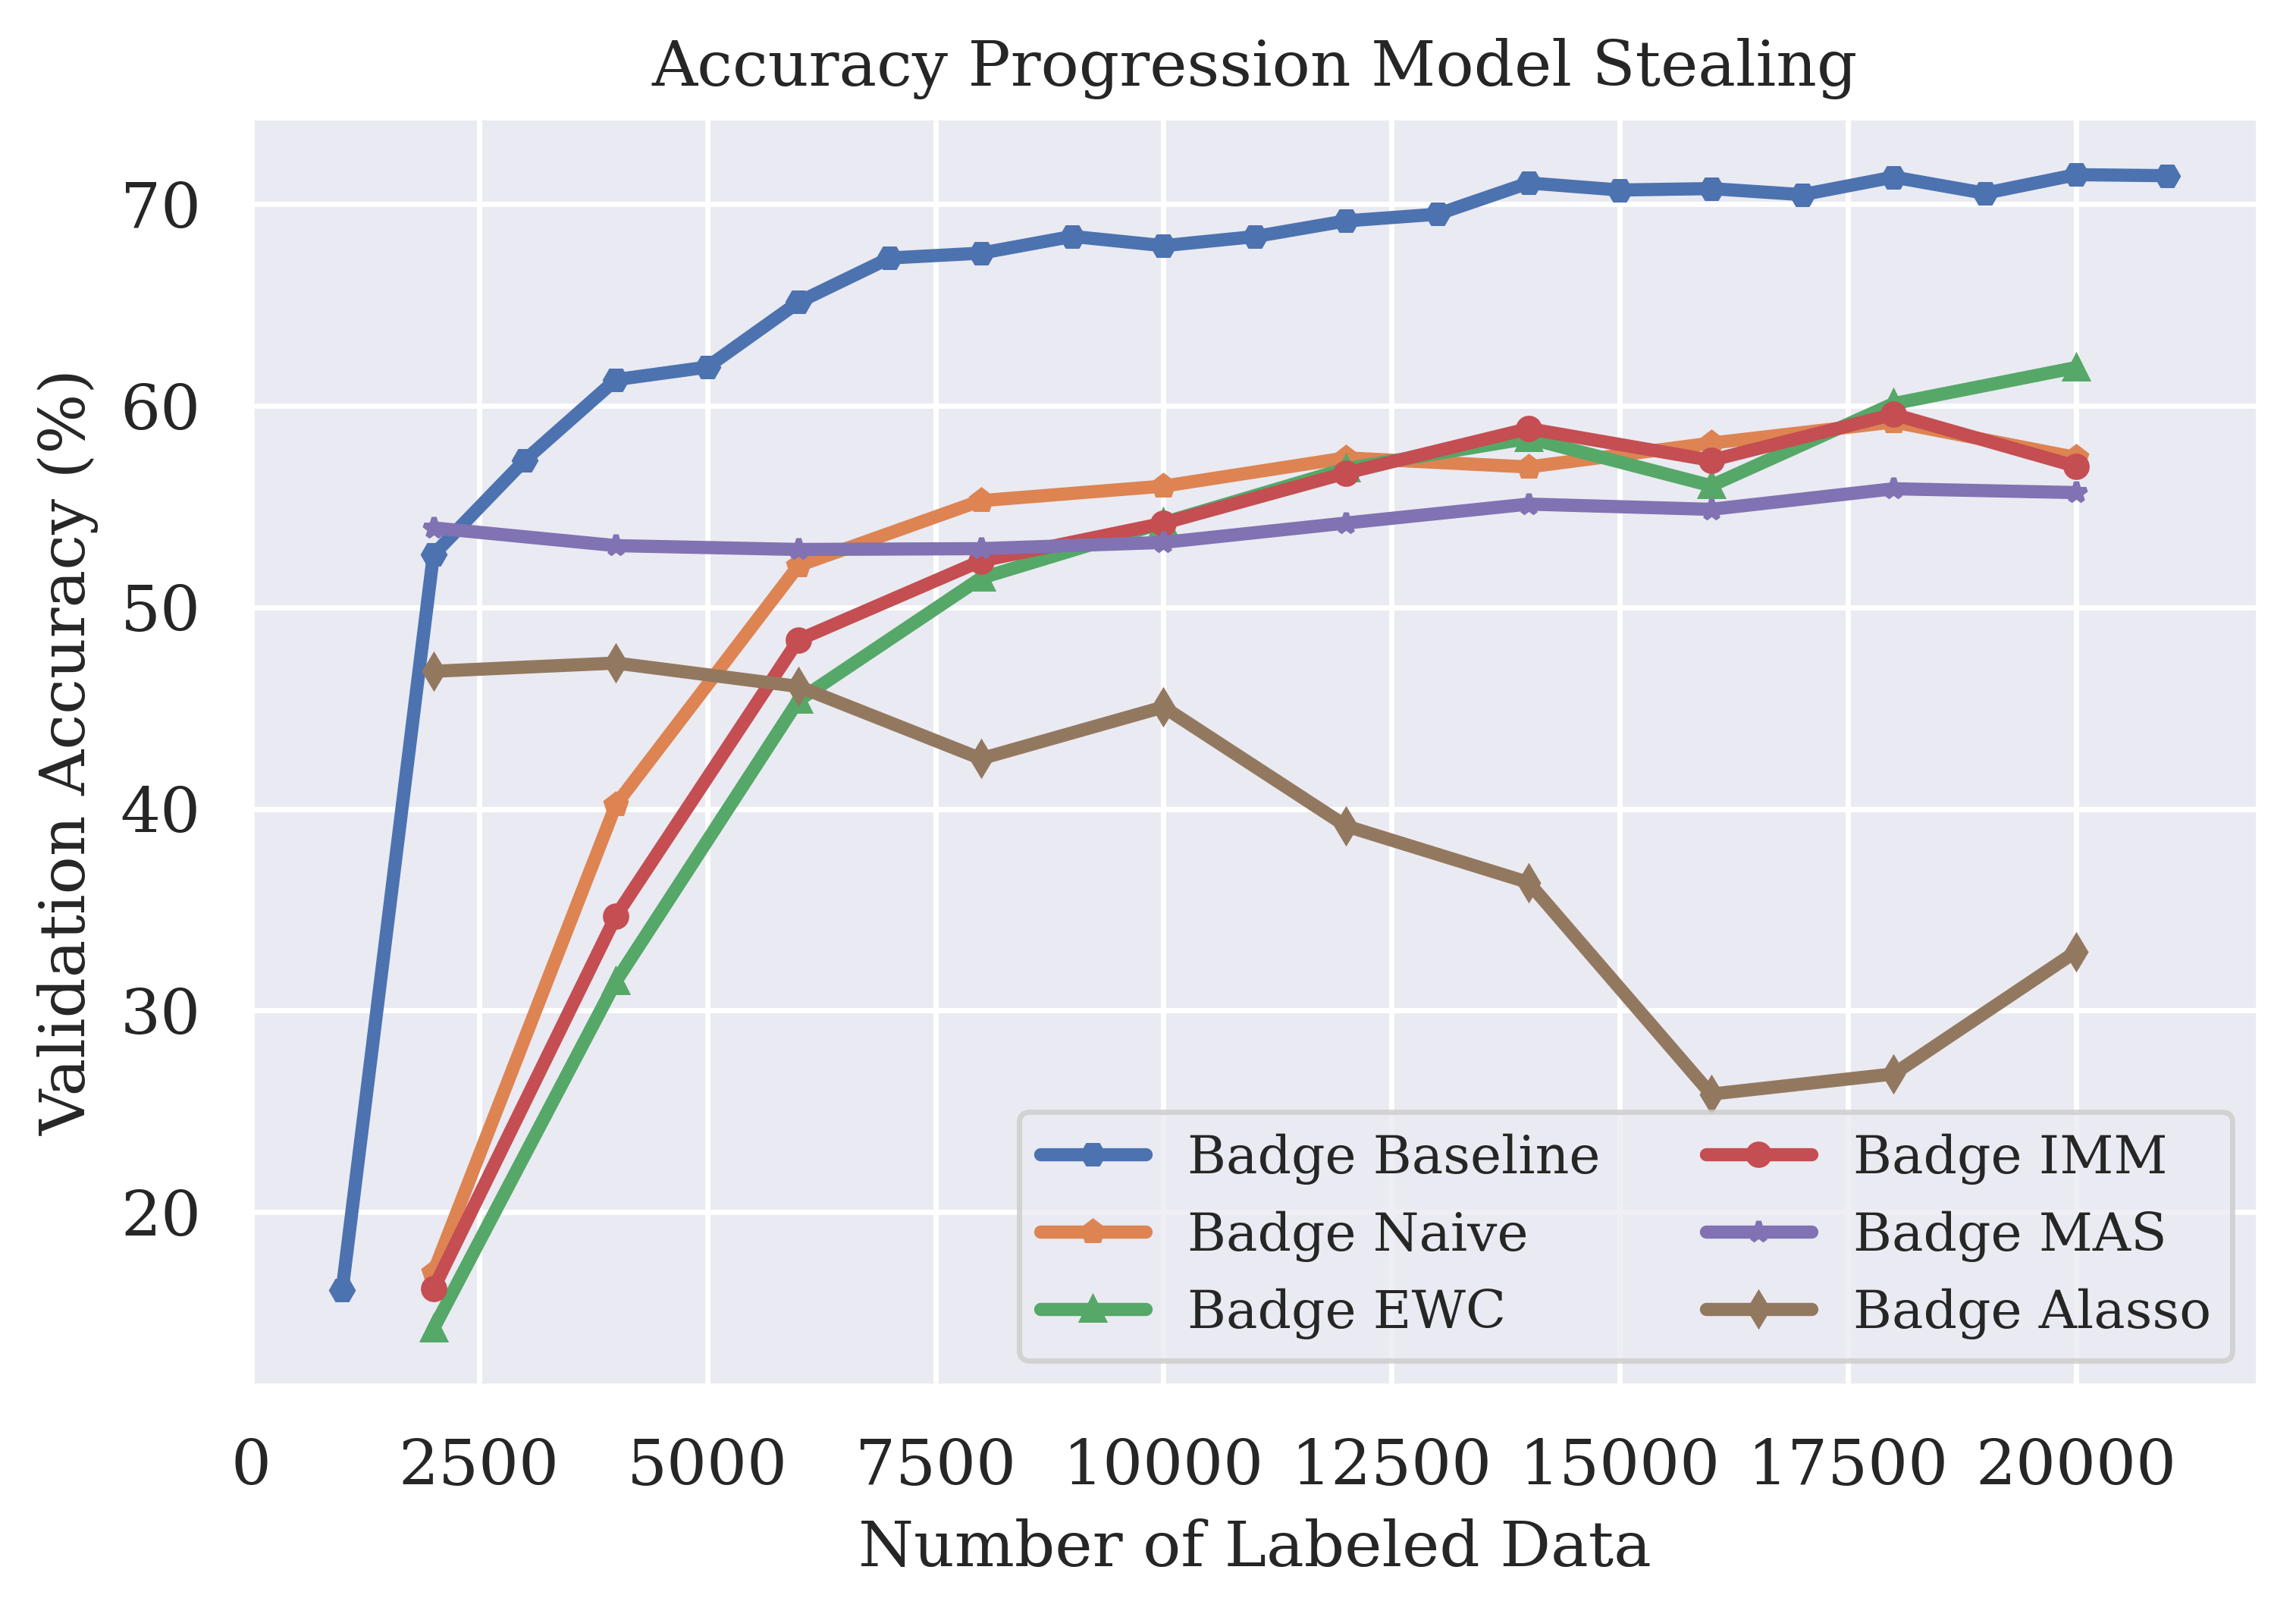
\includegraphics[width=0.7\linewidth]{images/results_CALMS/cifar_softmax_badge.png}
    \caption[Agreement Comparison for Model Stealing on CIFAR-10 using the softmax output and the Active Learning strategy Badge]{Progression of Model Agreement
    (in \%) for Model Stealing Attacks using Continual Active Learning on the CIFAR-10 dataset. We use Model Stealing Attacks with the Active Learning strategy
    \gls{badge} and train using the softmax output of the Target Model.}
    \label{fig:CALMSCIFAR10SoftmaxBadge}
\end{figure}


%Tables for MNIST
%Label
\begin{figure}[h]
    \centering
    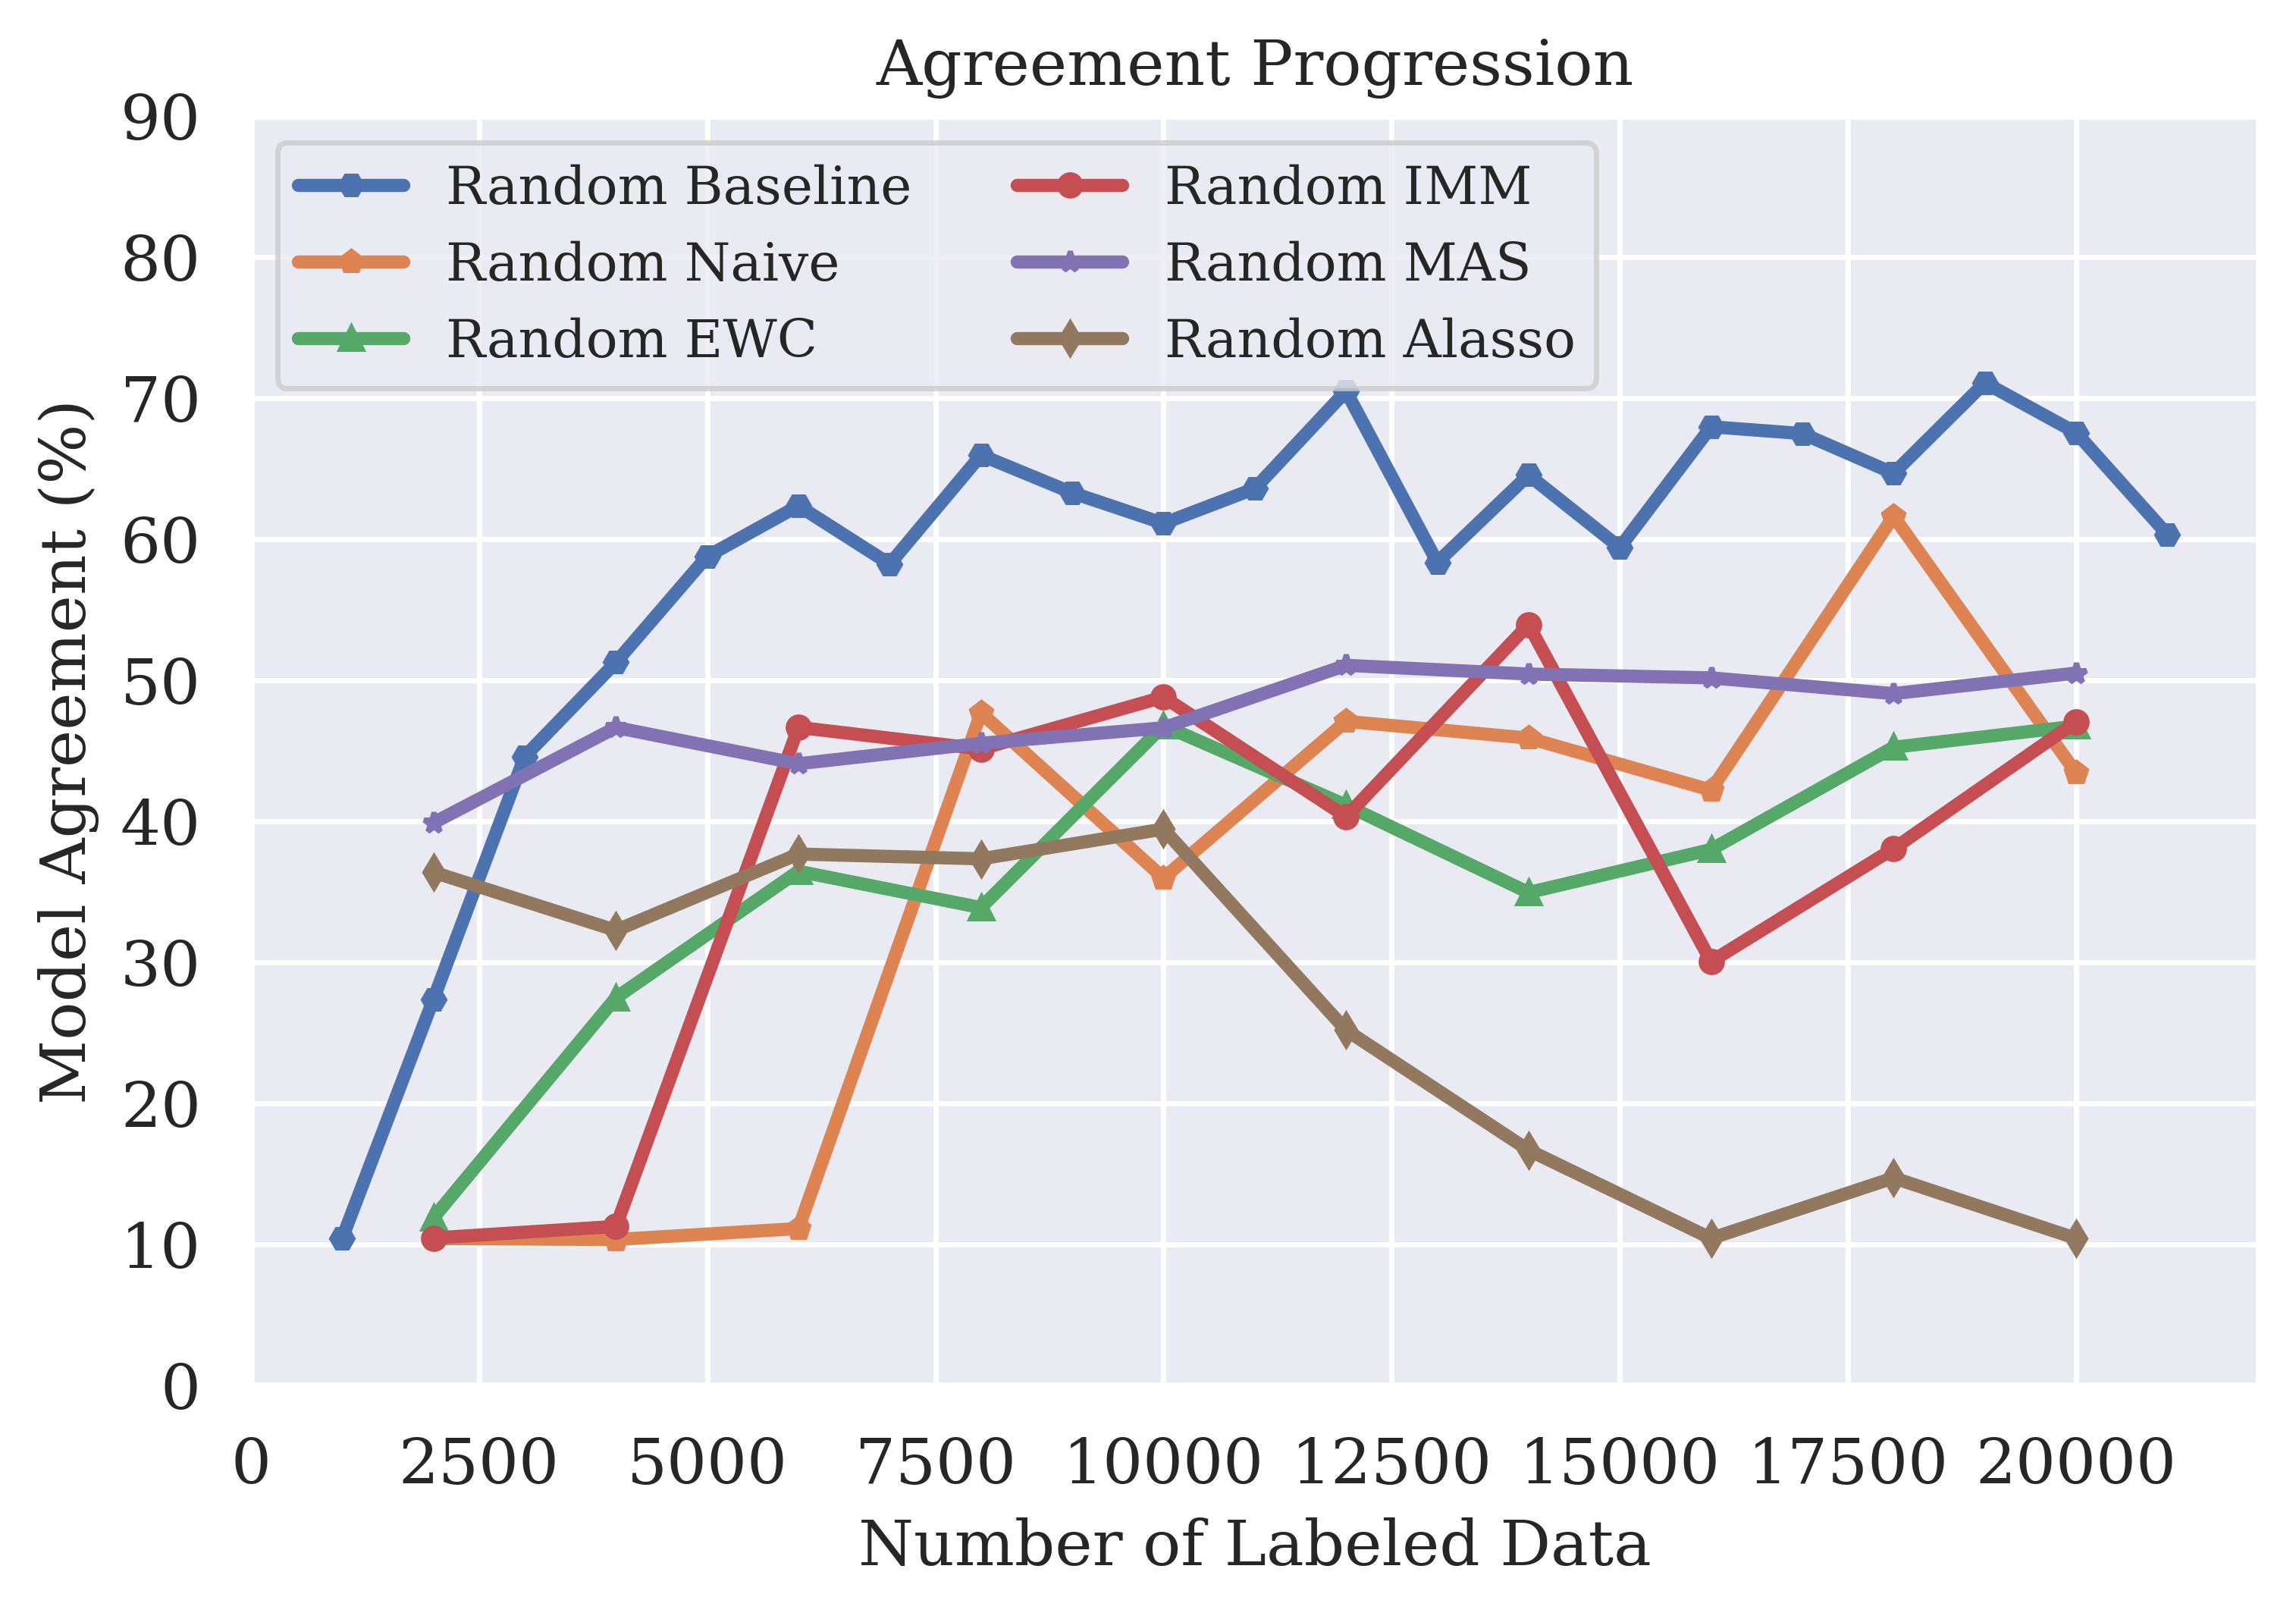
\includegraphics[width=0.7\linewidth]{images/results_CALMS/mnist_label_random.png}
    \caption[Agreement Comparison for Model Stealing on MNIST using the predicted class label and the Active Learning strategy Random]{Progression of Model Agreement
    (in \%) for Model Stealing Attacks using Continual Active Learning on the MNIST dataset. We use Model Stealing Attacks with the random sampling
    and train using the predicted class label of the Target Model.}
    \label{fig:CALMSMNISTLabelRandom}
\end{figure}

\begin{figure}[h]
    \centering
    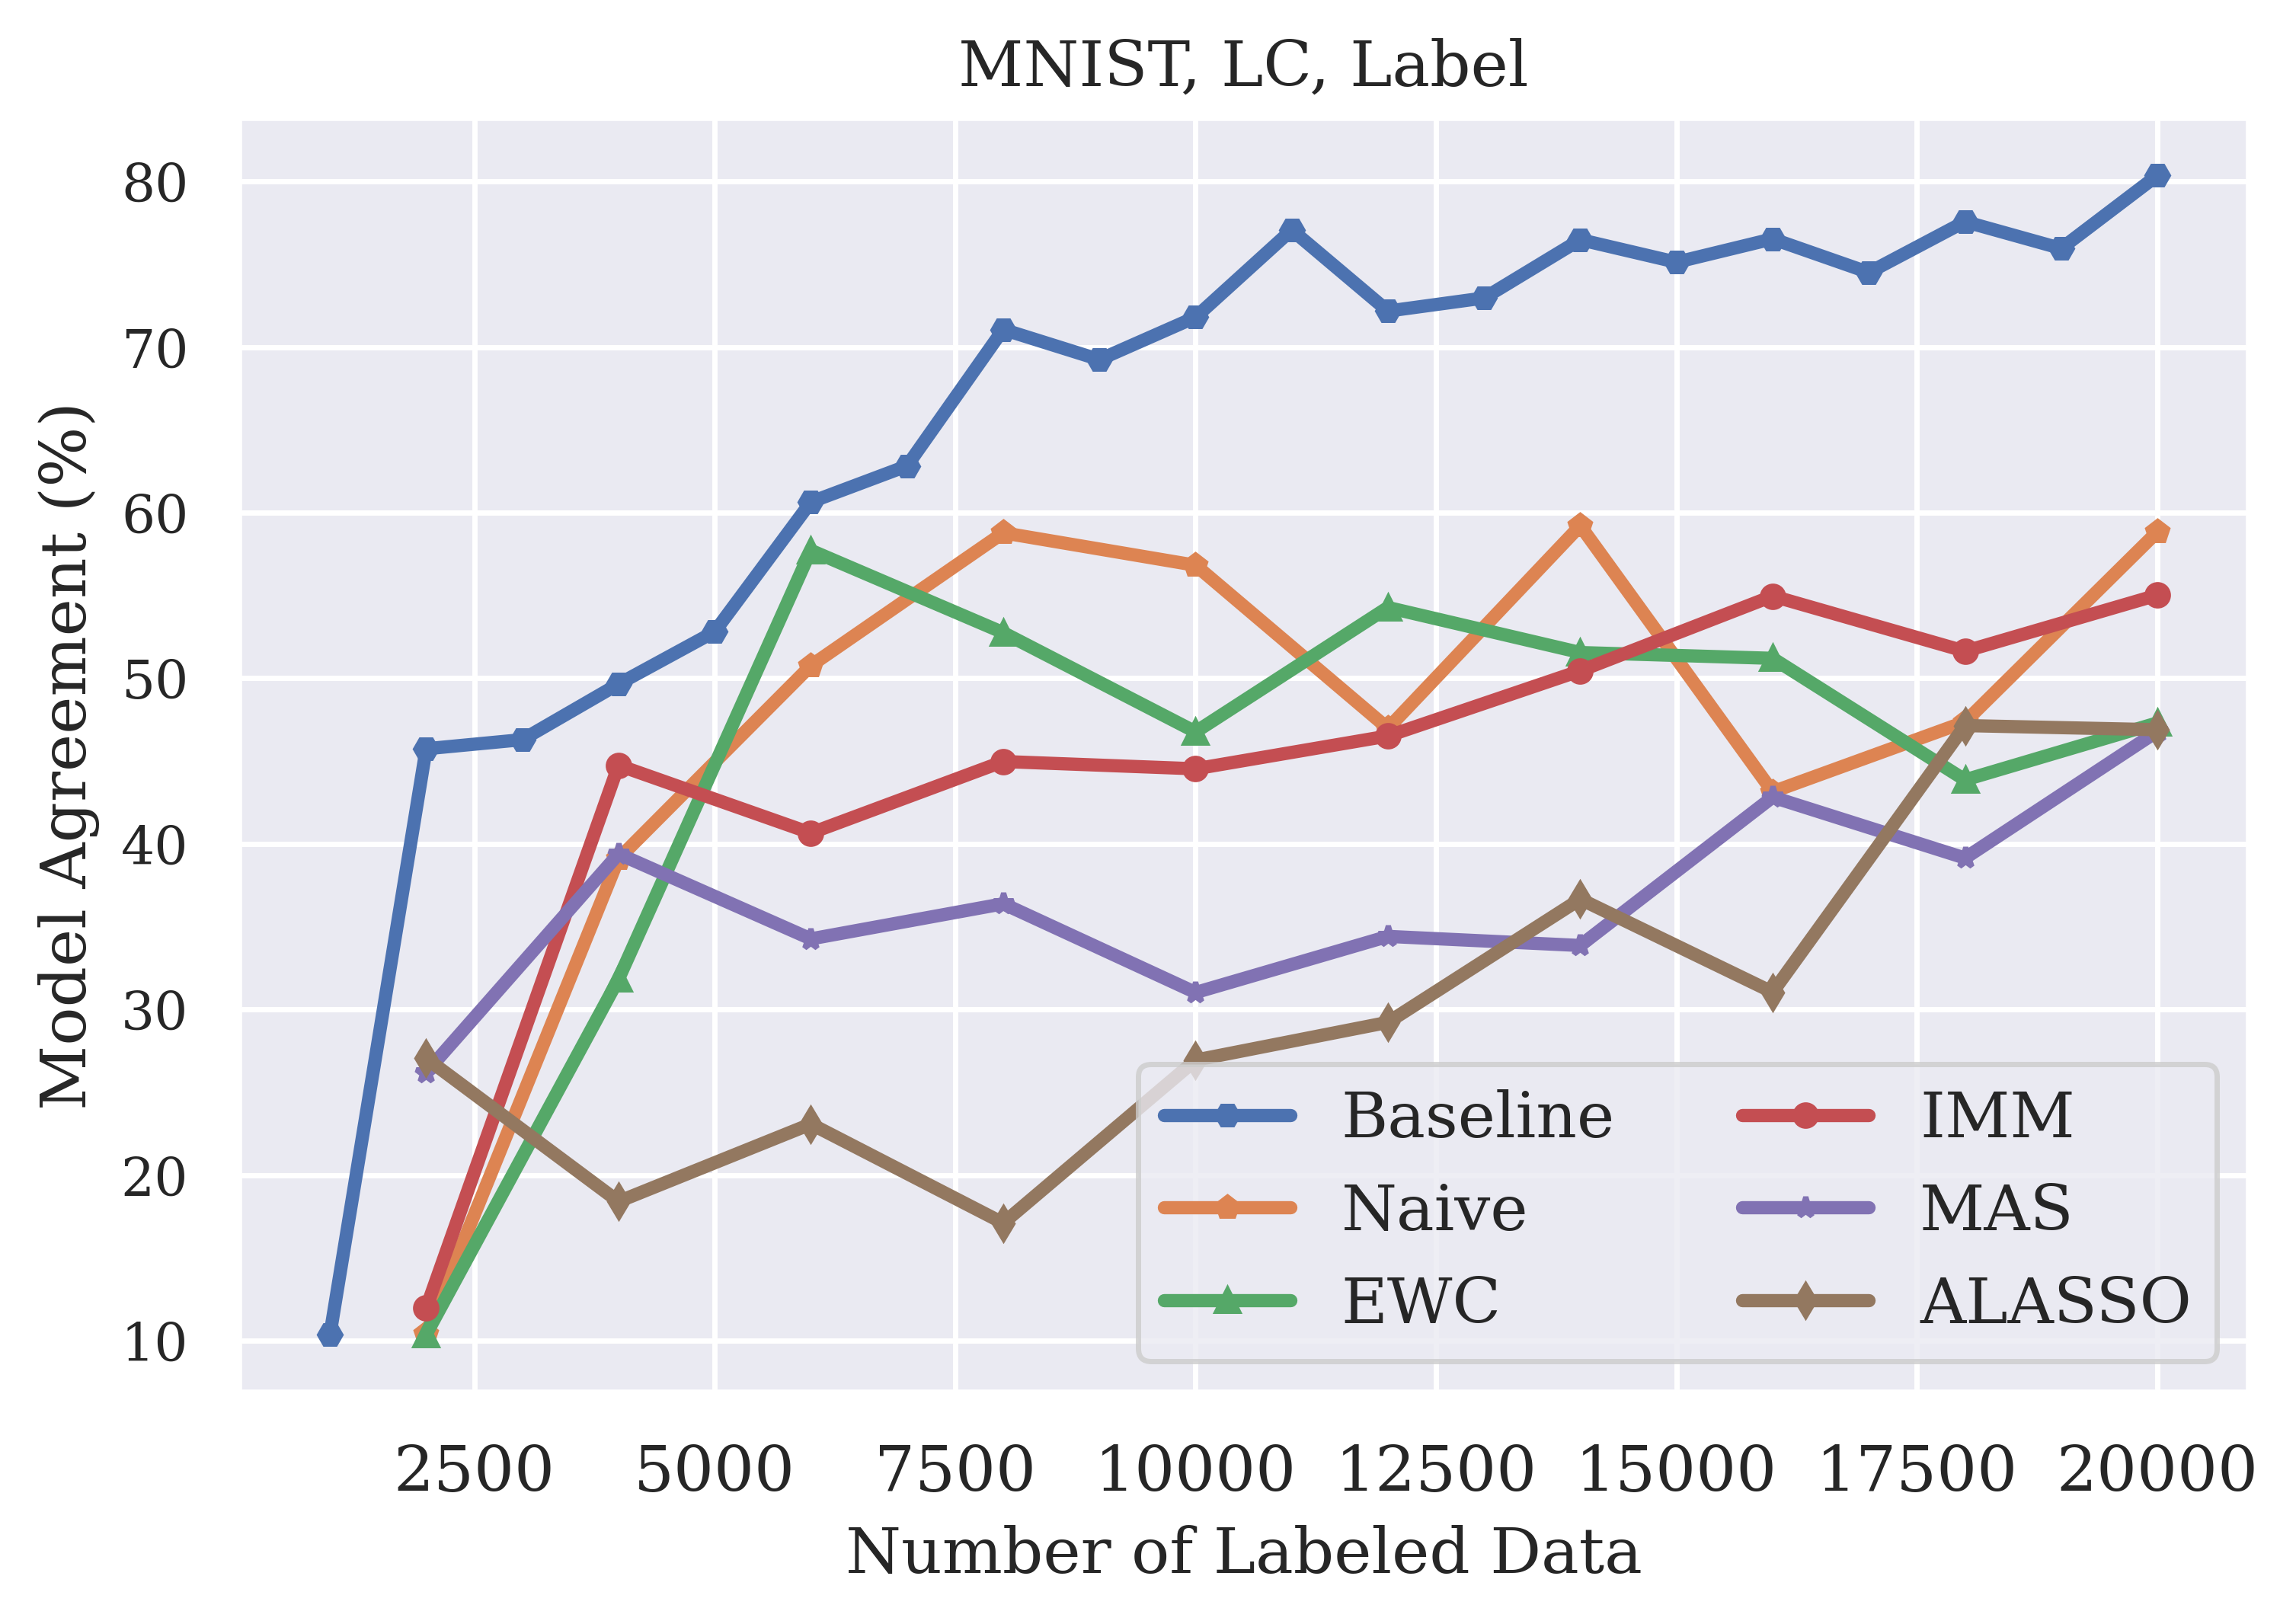
\includegraphics[width=0.7\linewidth]{images/results_CALMS/mnist_label_lc.png}
    \caption[Agreement Comparison for Model Stealing on MNIST using the predicted class label and the Active Learning strategy LC]{Progression of Model Agreement
    (in \%) for Model Stealing Attacks using Continual Active Learning on the MNIST dataset. We use Model Stealing Attacks with the Active Learning strategy
    \gls{lc} and train using the predicted class label of the Target Model.}
    \label{fig:CALMSMNISTLabelLC}
\end{figure}

\begin{figure}[h]
    \centering
    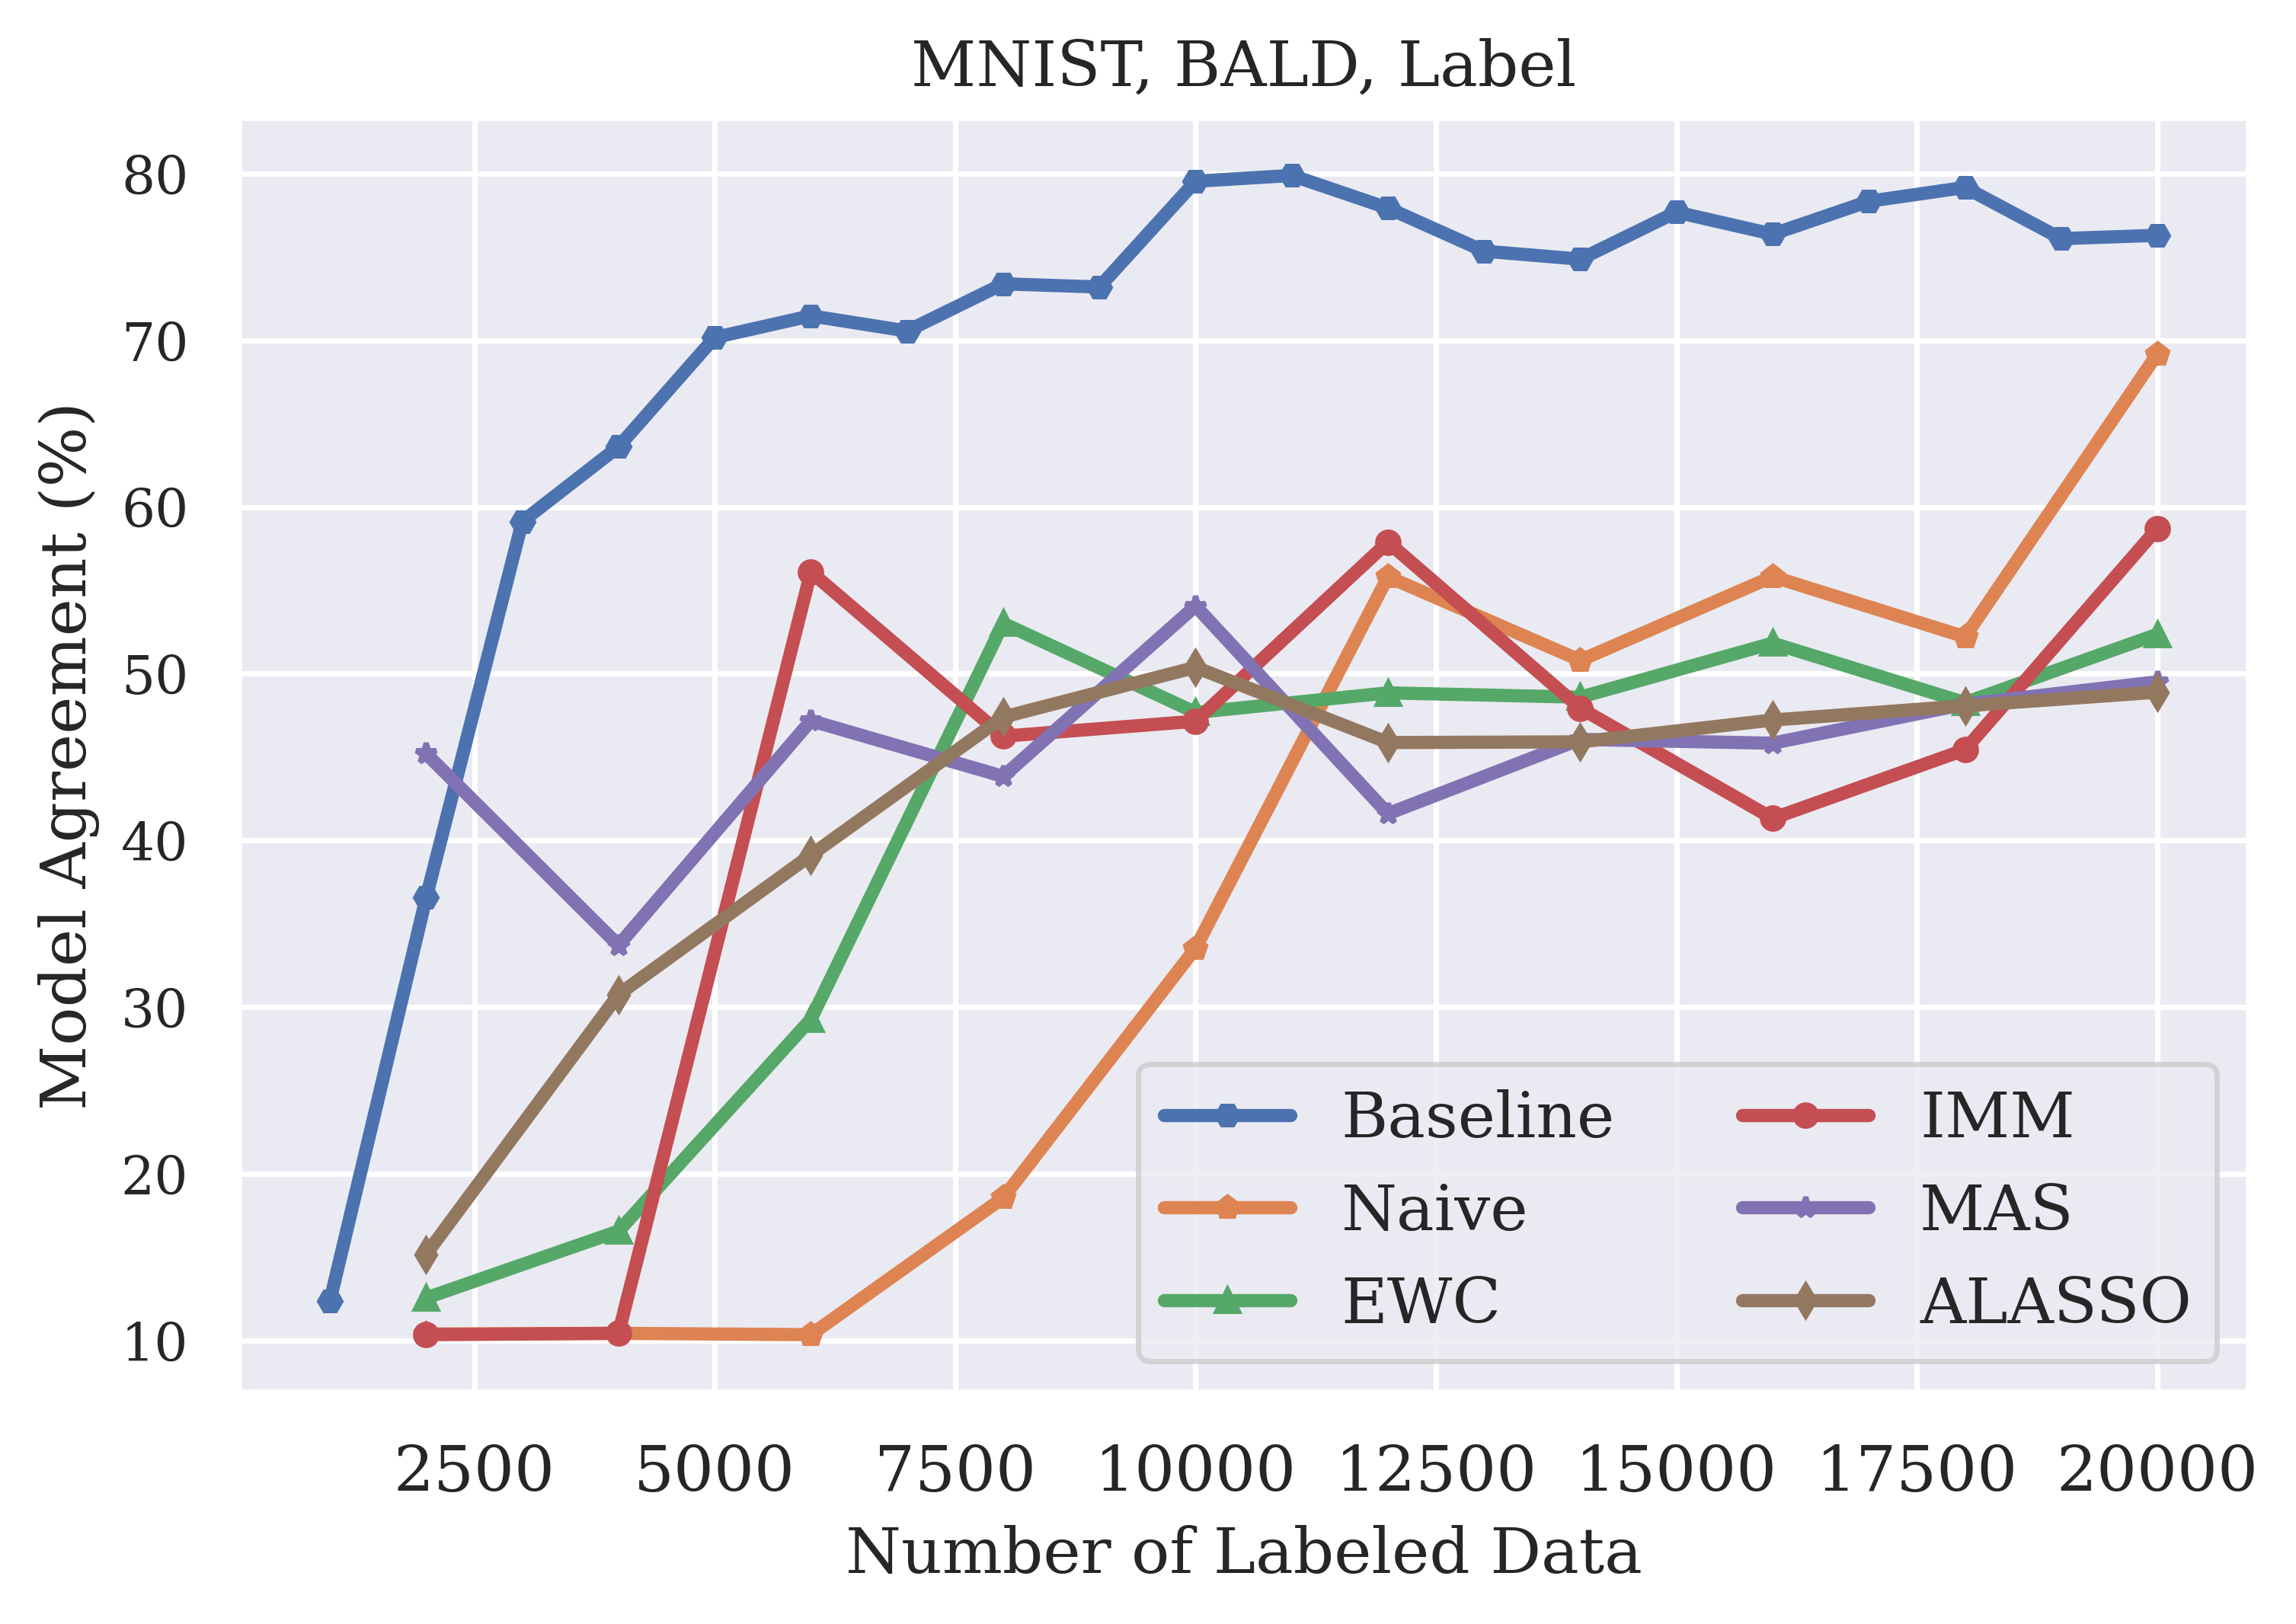
\includegraphics[width=0.7\linewidth]{images/results_CALMS/mnist_label_bald.png}
    \caption[Accuracy Comparison for Model Stealing on MNIST using the predicted class label and the Active Learning strategy BALD]{Progression of Model Agreement
    (in \%) for Model Stealing Attacks using Continual Active Learning on the MNIST dataset. We use Model Stealing Attacks with the Active Learning strategy
    \gls{bald} and train using the predicted class label of the Target Model.}
    \label{fig:CALMSMNISTLabelBALD}
\end{figure}

\begin{figure}[h]
    \centering
    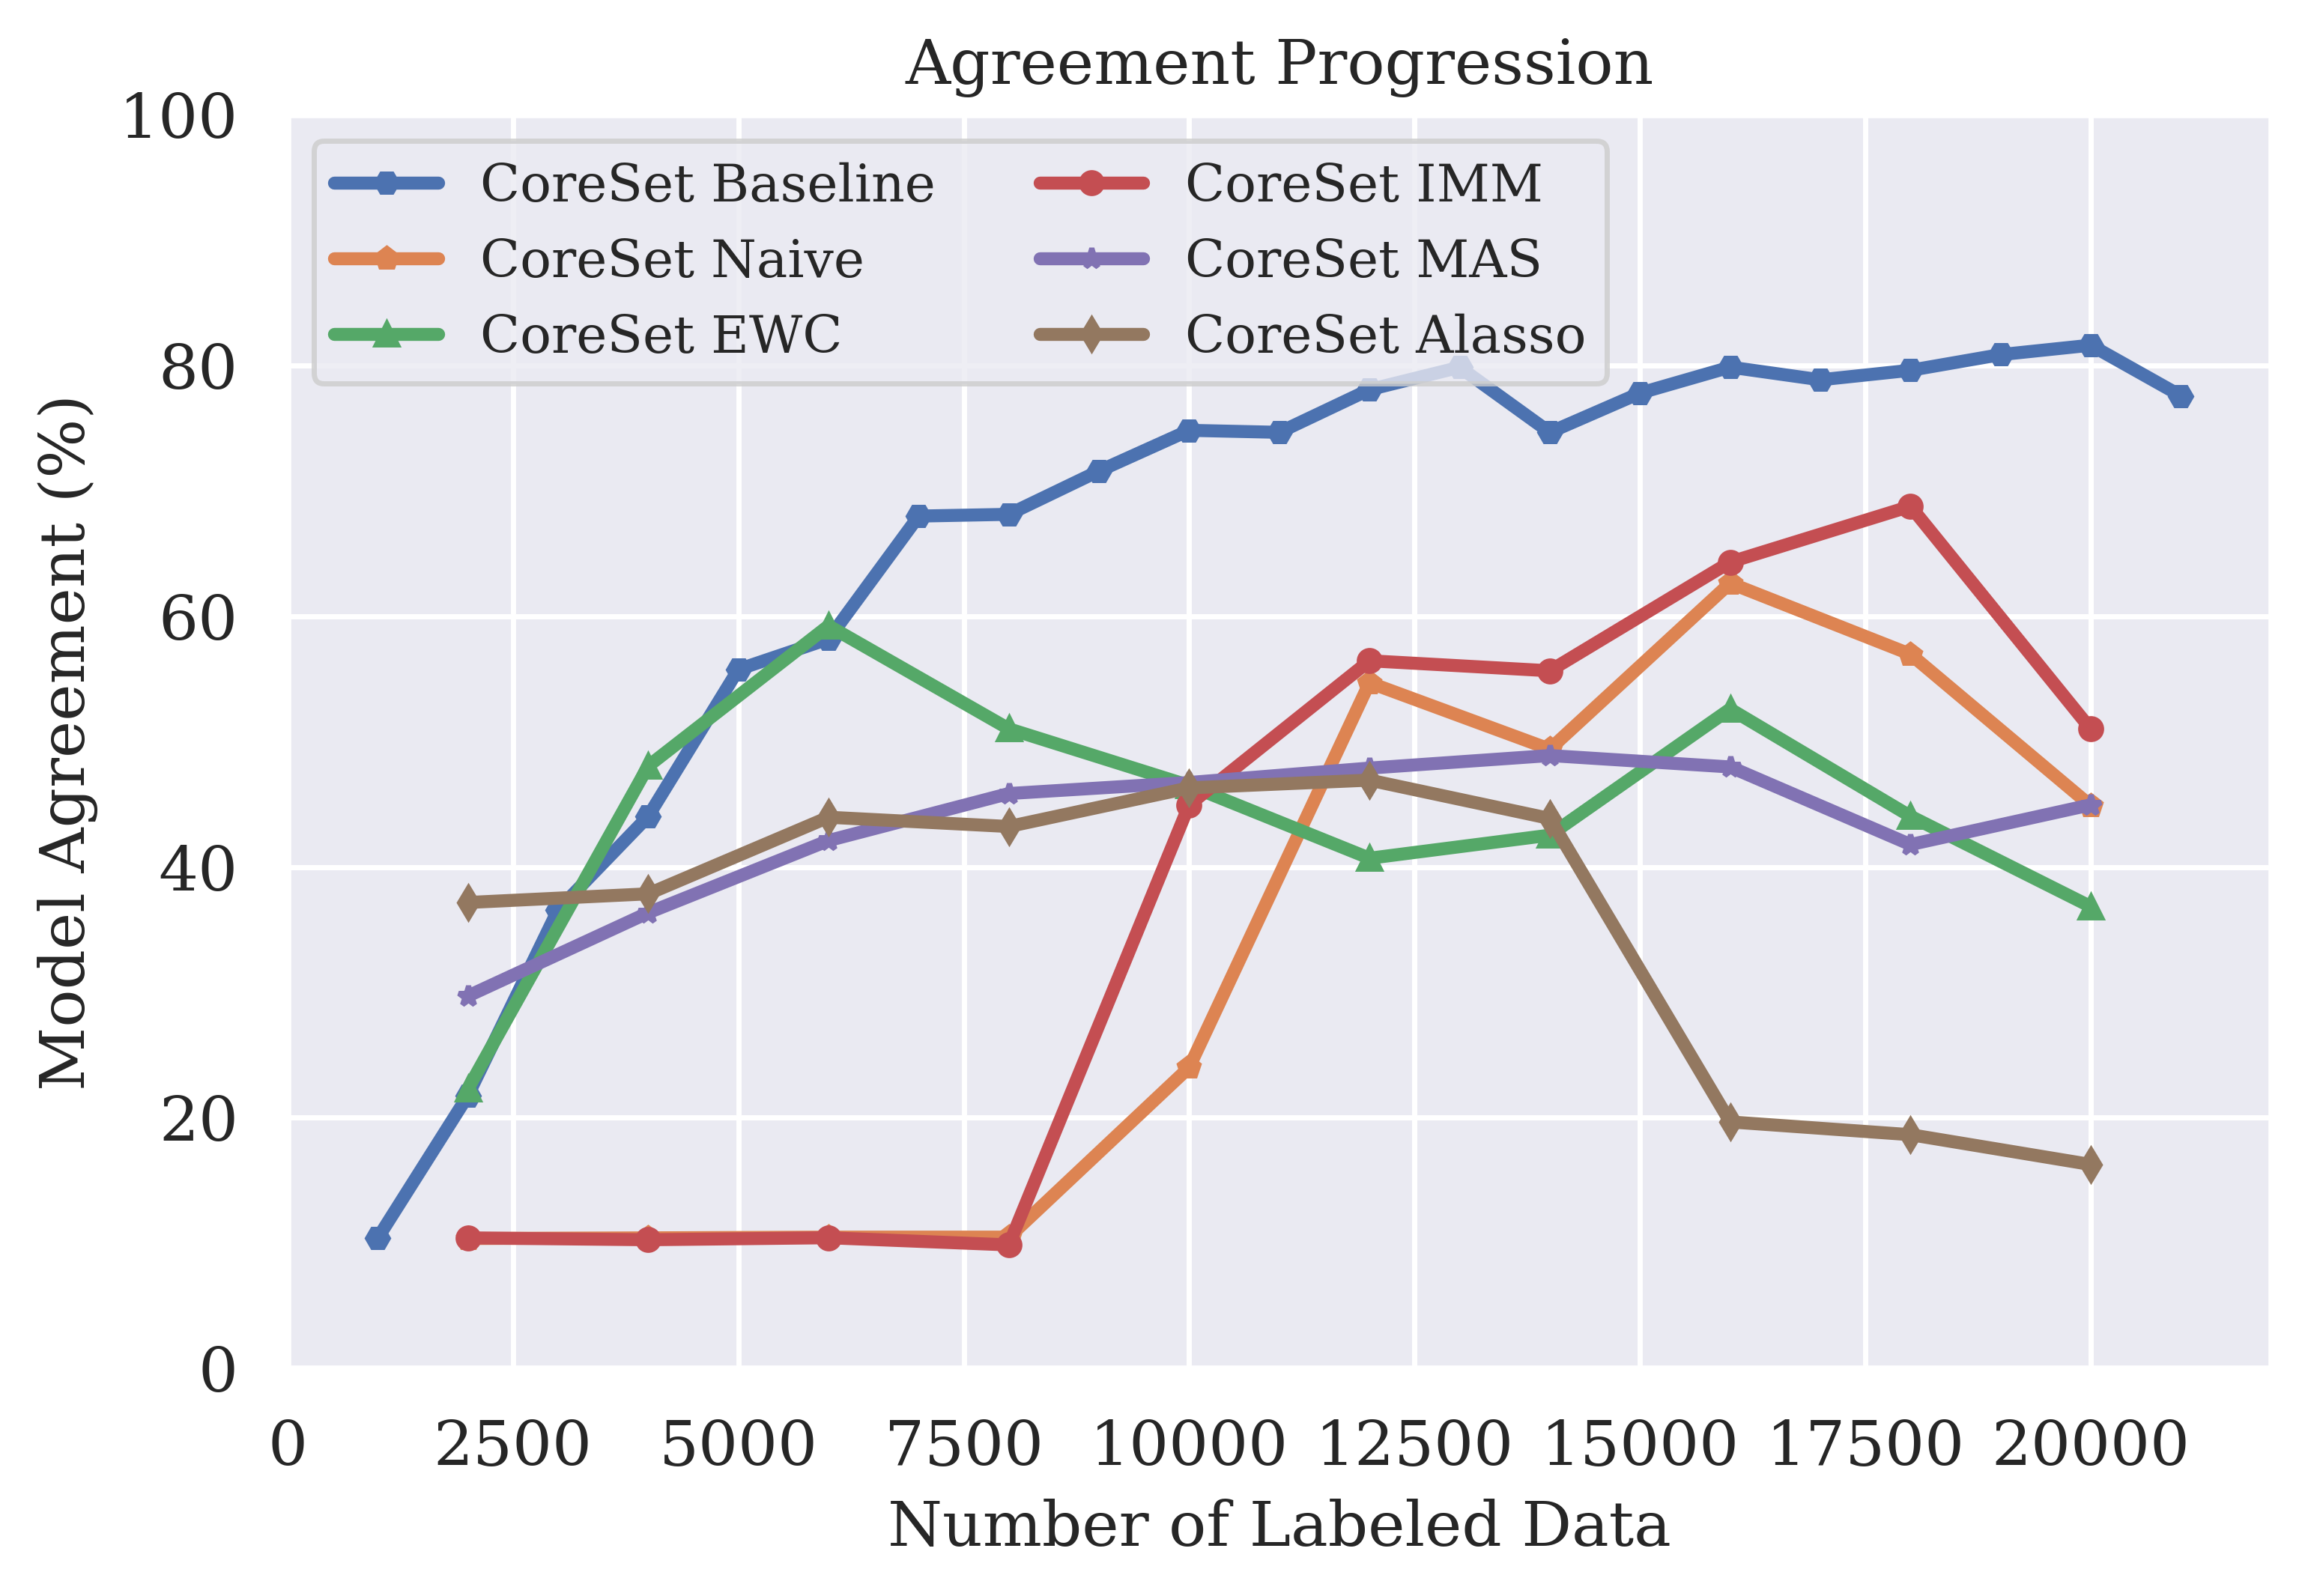
\includegraphics[width=0.7\linewidth]{images/results_CALMS/mnist_label_coreset.png}
    \caption[Agreement Comparison for Model Stealing on MNIST using the predicted class label and the Active Learning strategy CoreSet]{Progression of Model Agreement
    (in \%) for Model Stealing Attacks using Continual Active Learning on the MNIST dataset. We use Model Stealing Attacks with the Active Learning strategy
    CoreSet and train using the predicted class label of the Target Model.}
    \label{fig:CALMSMNISTLabelCoreSet}
\end{figure}

\begin{figure}[h]
    \centering
    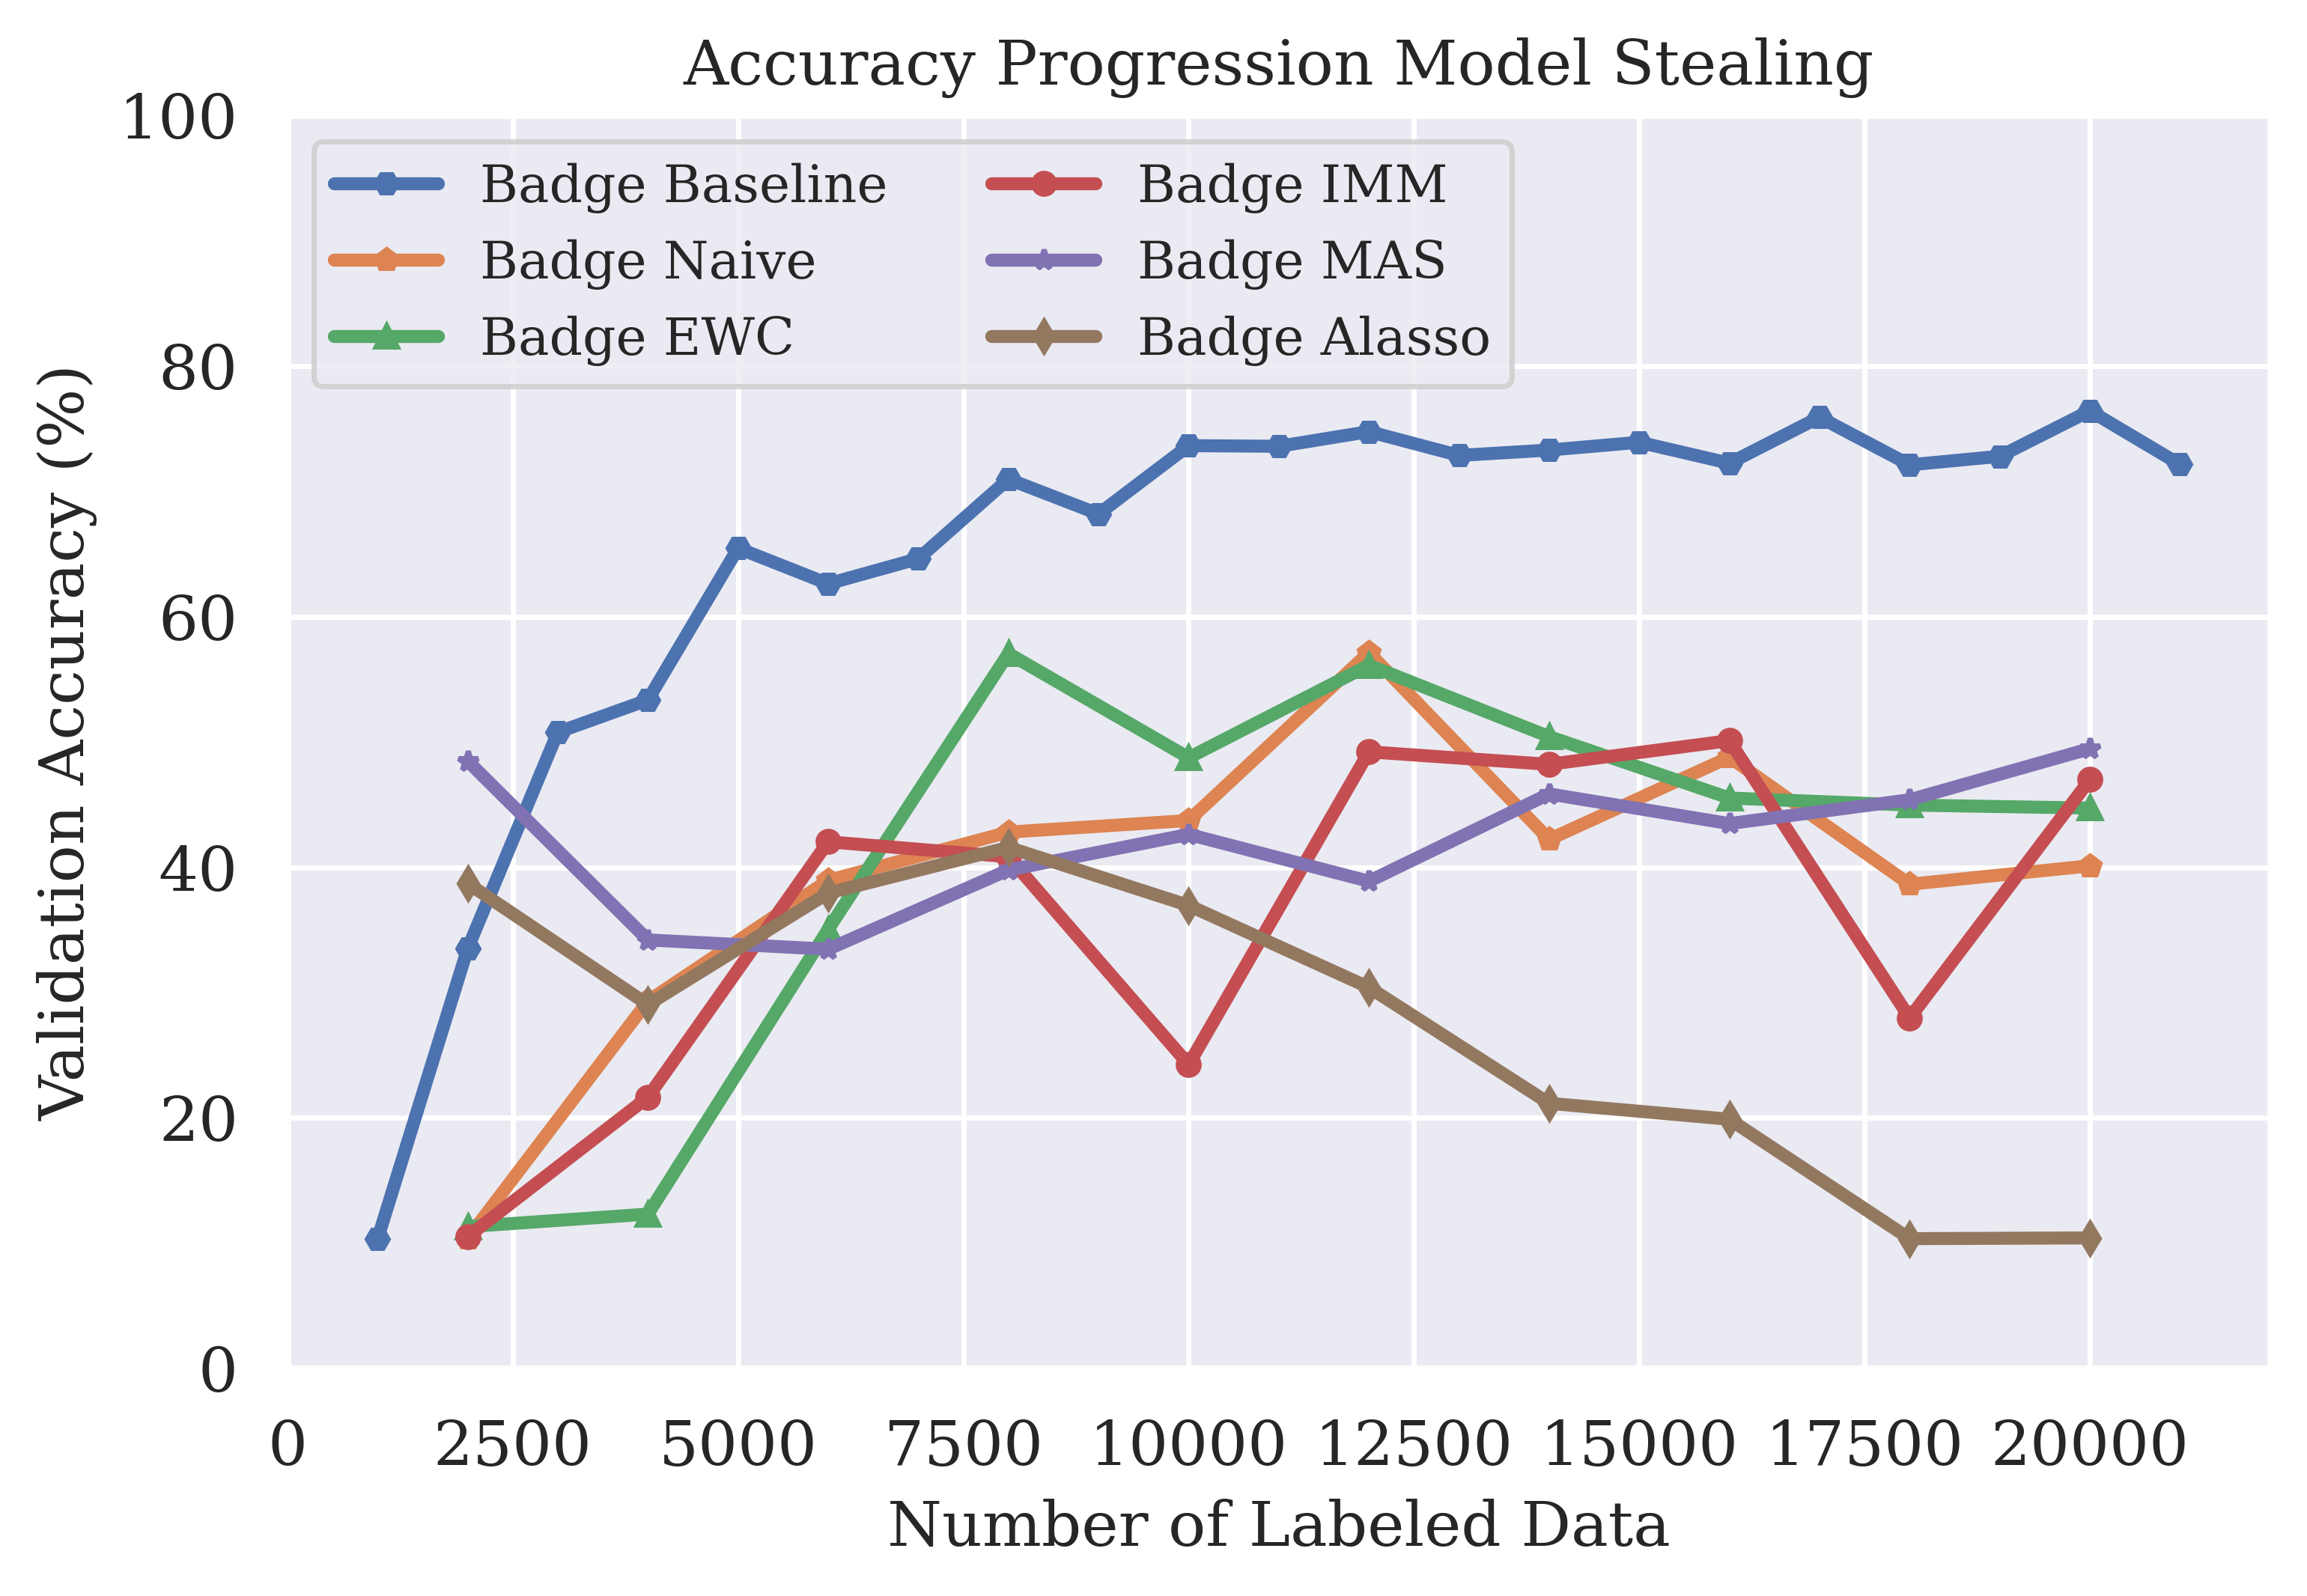
\includegraphics[width=0.7\linewidth]{images/results_CALMS/mnist_label_badge.png}
    \caption[Agreement Comparison for Model Stealing on MNIST using the predicted class label and the Active Learning strategy Badge]{Progression of Model Agreement
    (in \%) for Model Stealing Attacks using Continual Active Learning on the MNIST dataset. We use Model Stealing Attacks with the Active Learning strategy
    \gls{badge} and train using the predicted class label of the Target Model.}
    \label{fig:CALMSMNISTLabelBadge}
\end{figure}

%Softmax
\begin{figure}[h]
    \centering
    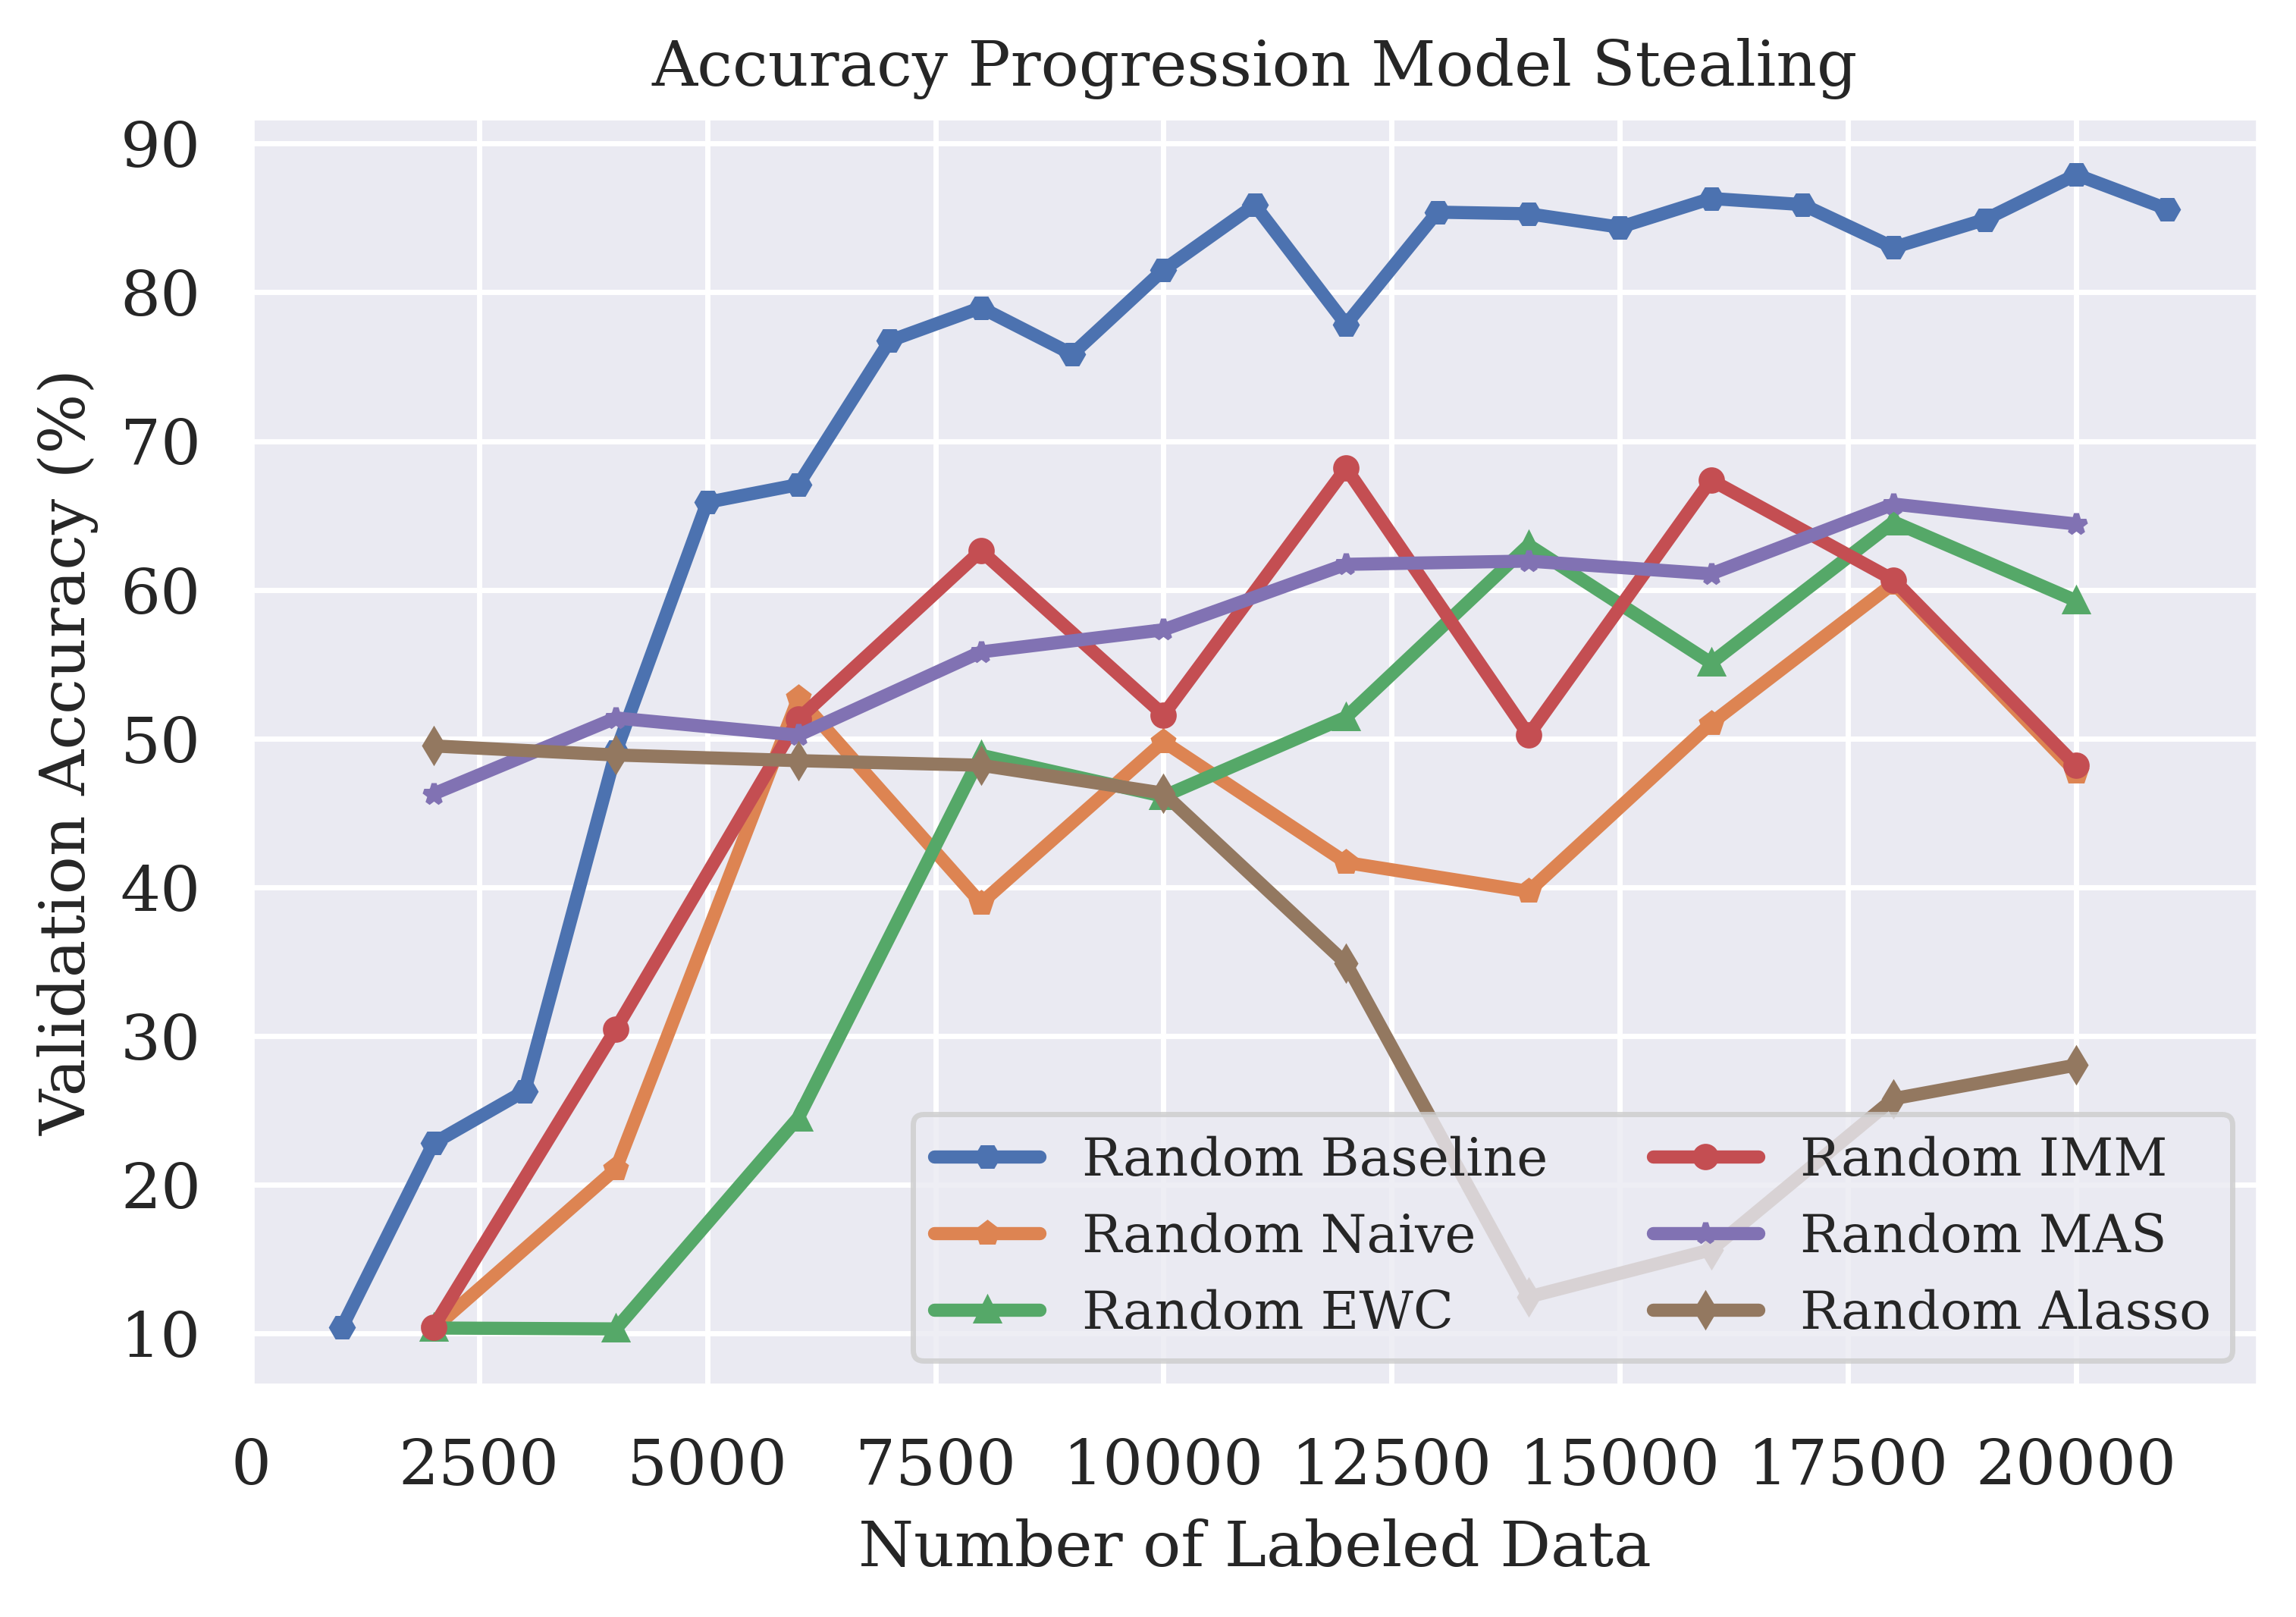
\includegraphics[width=0.7\linewidth]{images/results_CALMS/mnist_softmax_random.png}
    \caption[Agreement Comparison for Model Stealing on MNIST using the softmax output and the Active Learning strategy Random]{Progression of Model Agreement
    (in \%) for Model Stealing Attacks using Continual Active Learning on the MNIST dataset. We use Model Stealing Attacks with random sampling and train
    using the softmax output of the Target Model.}
    \label{fig:CALMSMNISTSoftmaxRandom}
\end{figure}

\begin{figure}[h]
    \centering
    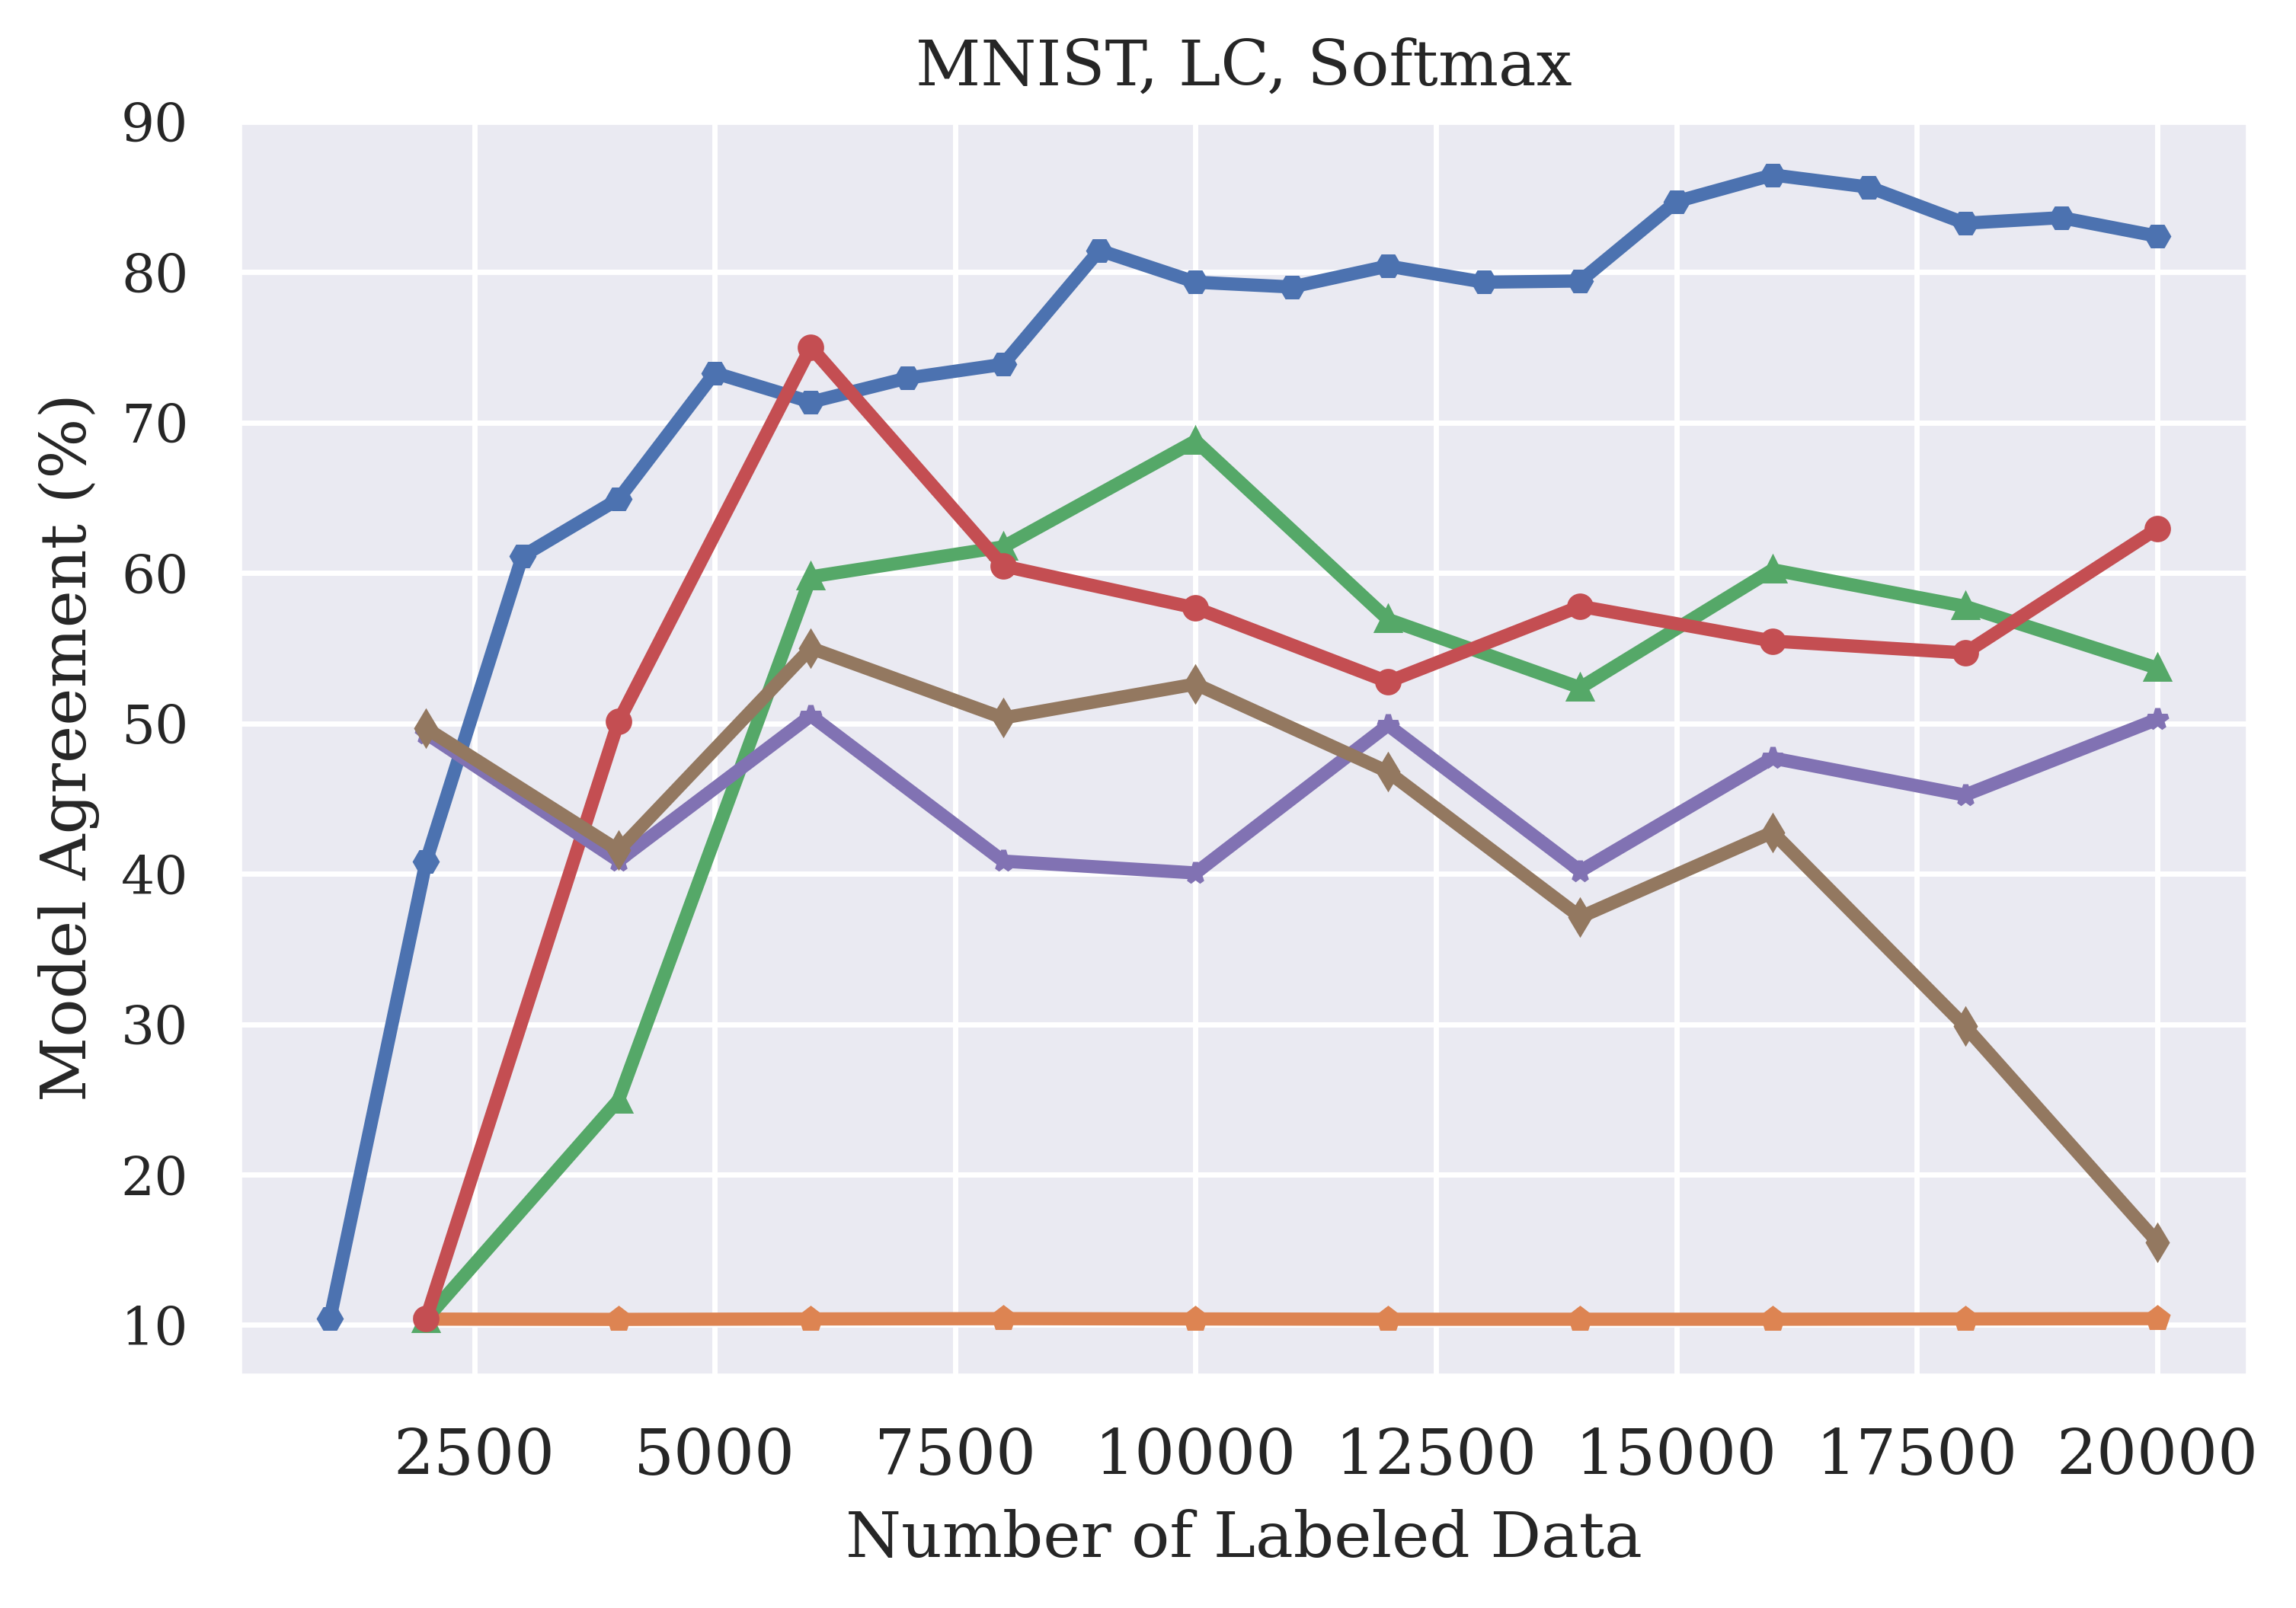
\includegraphics[width=0.7\linewidth]{images/results_CALMS/mnist_softmax_lc.png}
    \caption[Agreement Comparison for Model Stealing on MNIST using the softmax output and the Active Learning strategy LC]{Progression of Model Agreement
    (in \%) for Model Stealing Attacks using Continual Active Learning on the MNIST dataset. We use Model Stealing Attacks with the Active Learning strategy
    \gls{lc} and train using the softmax output of the Target Model.}
    \label{fig:CALMSMNISTSoftmaxLC}
\end{figure}

\begin{figure}[h]
    \centering
    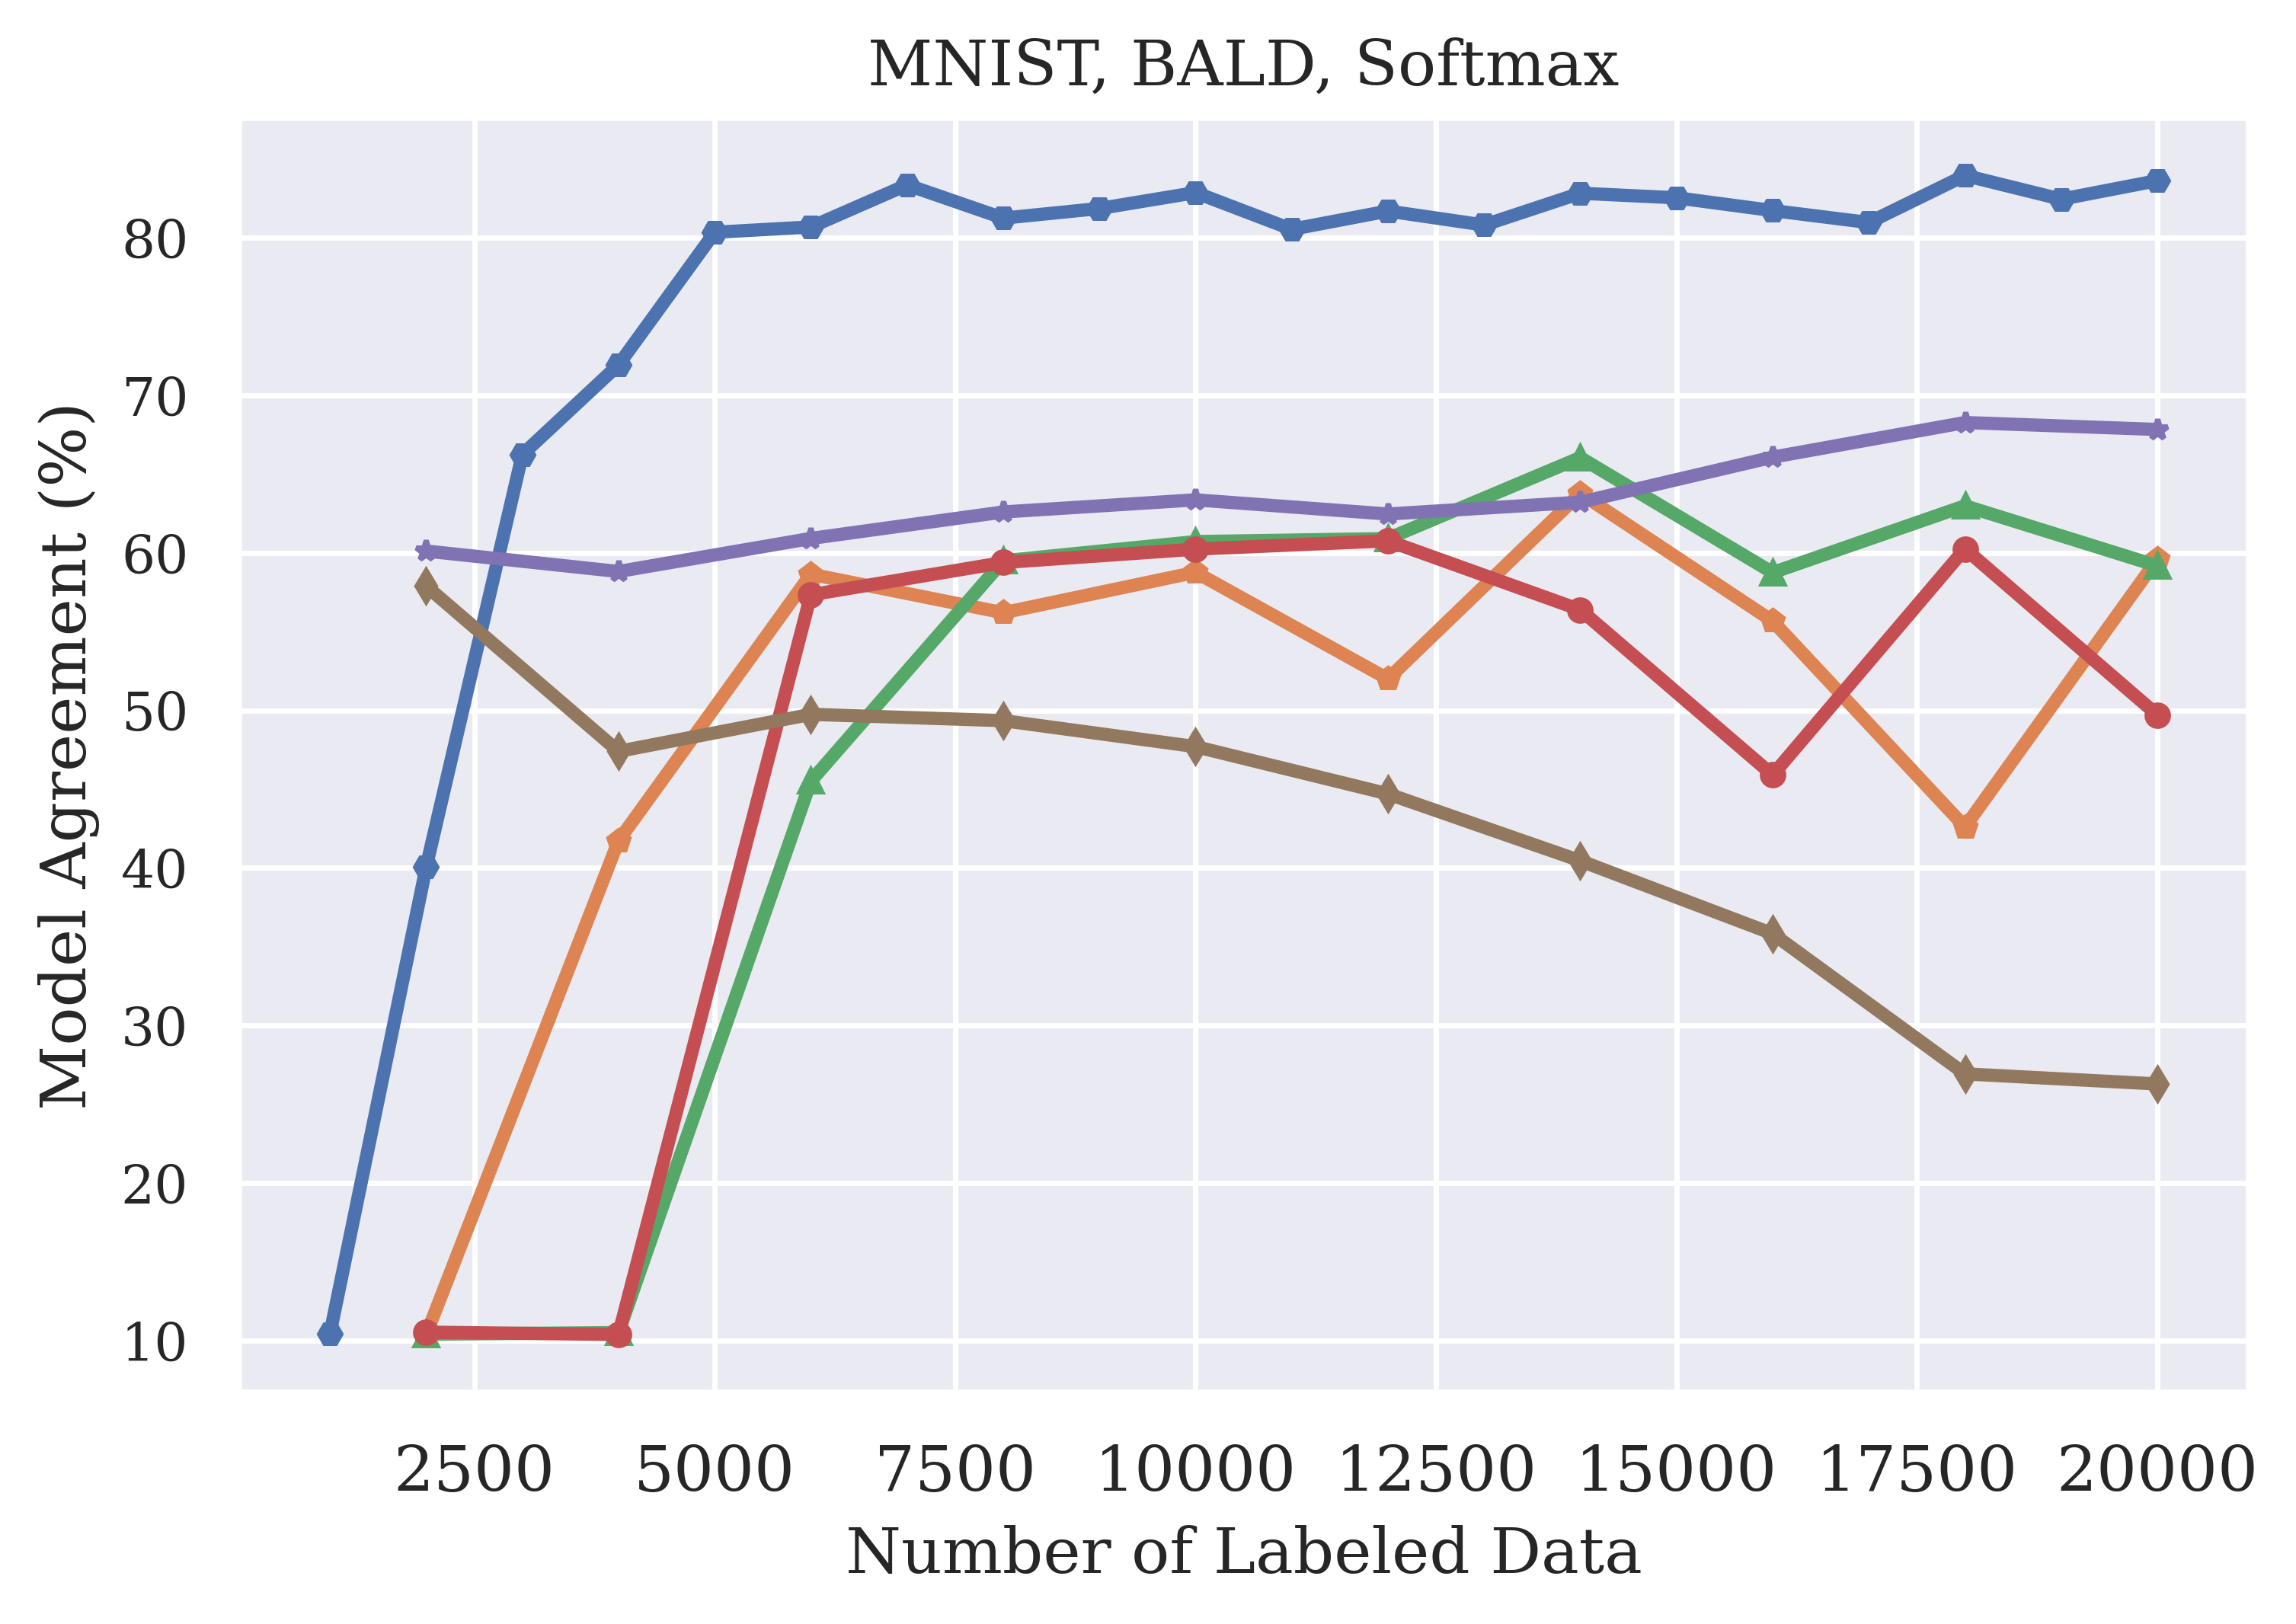
\includegraphics[width=0.7\linewidth]{images/results_CALMS/mnist_softmax_bald.png}
    \caption[Agreement Comparison for Model Stealing on MNIST using the softmax output and the Active Learning strategy BALD]{Progression of Model Agreement
    (in \%) for Model Stealing Attacks using Continual Active Learning on the MNIST dataset. We use Model Stealing Attacks with the Active Learning strategy
    \gls{bald} and train using the softmax output of the Target Model.}
    \label{fig:CALMSMNISTSoftmaxBALD}
\end{figure}

\begin{figure}[h]
    \centering
    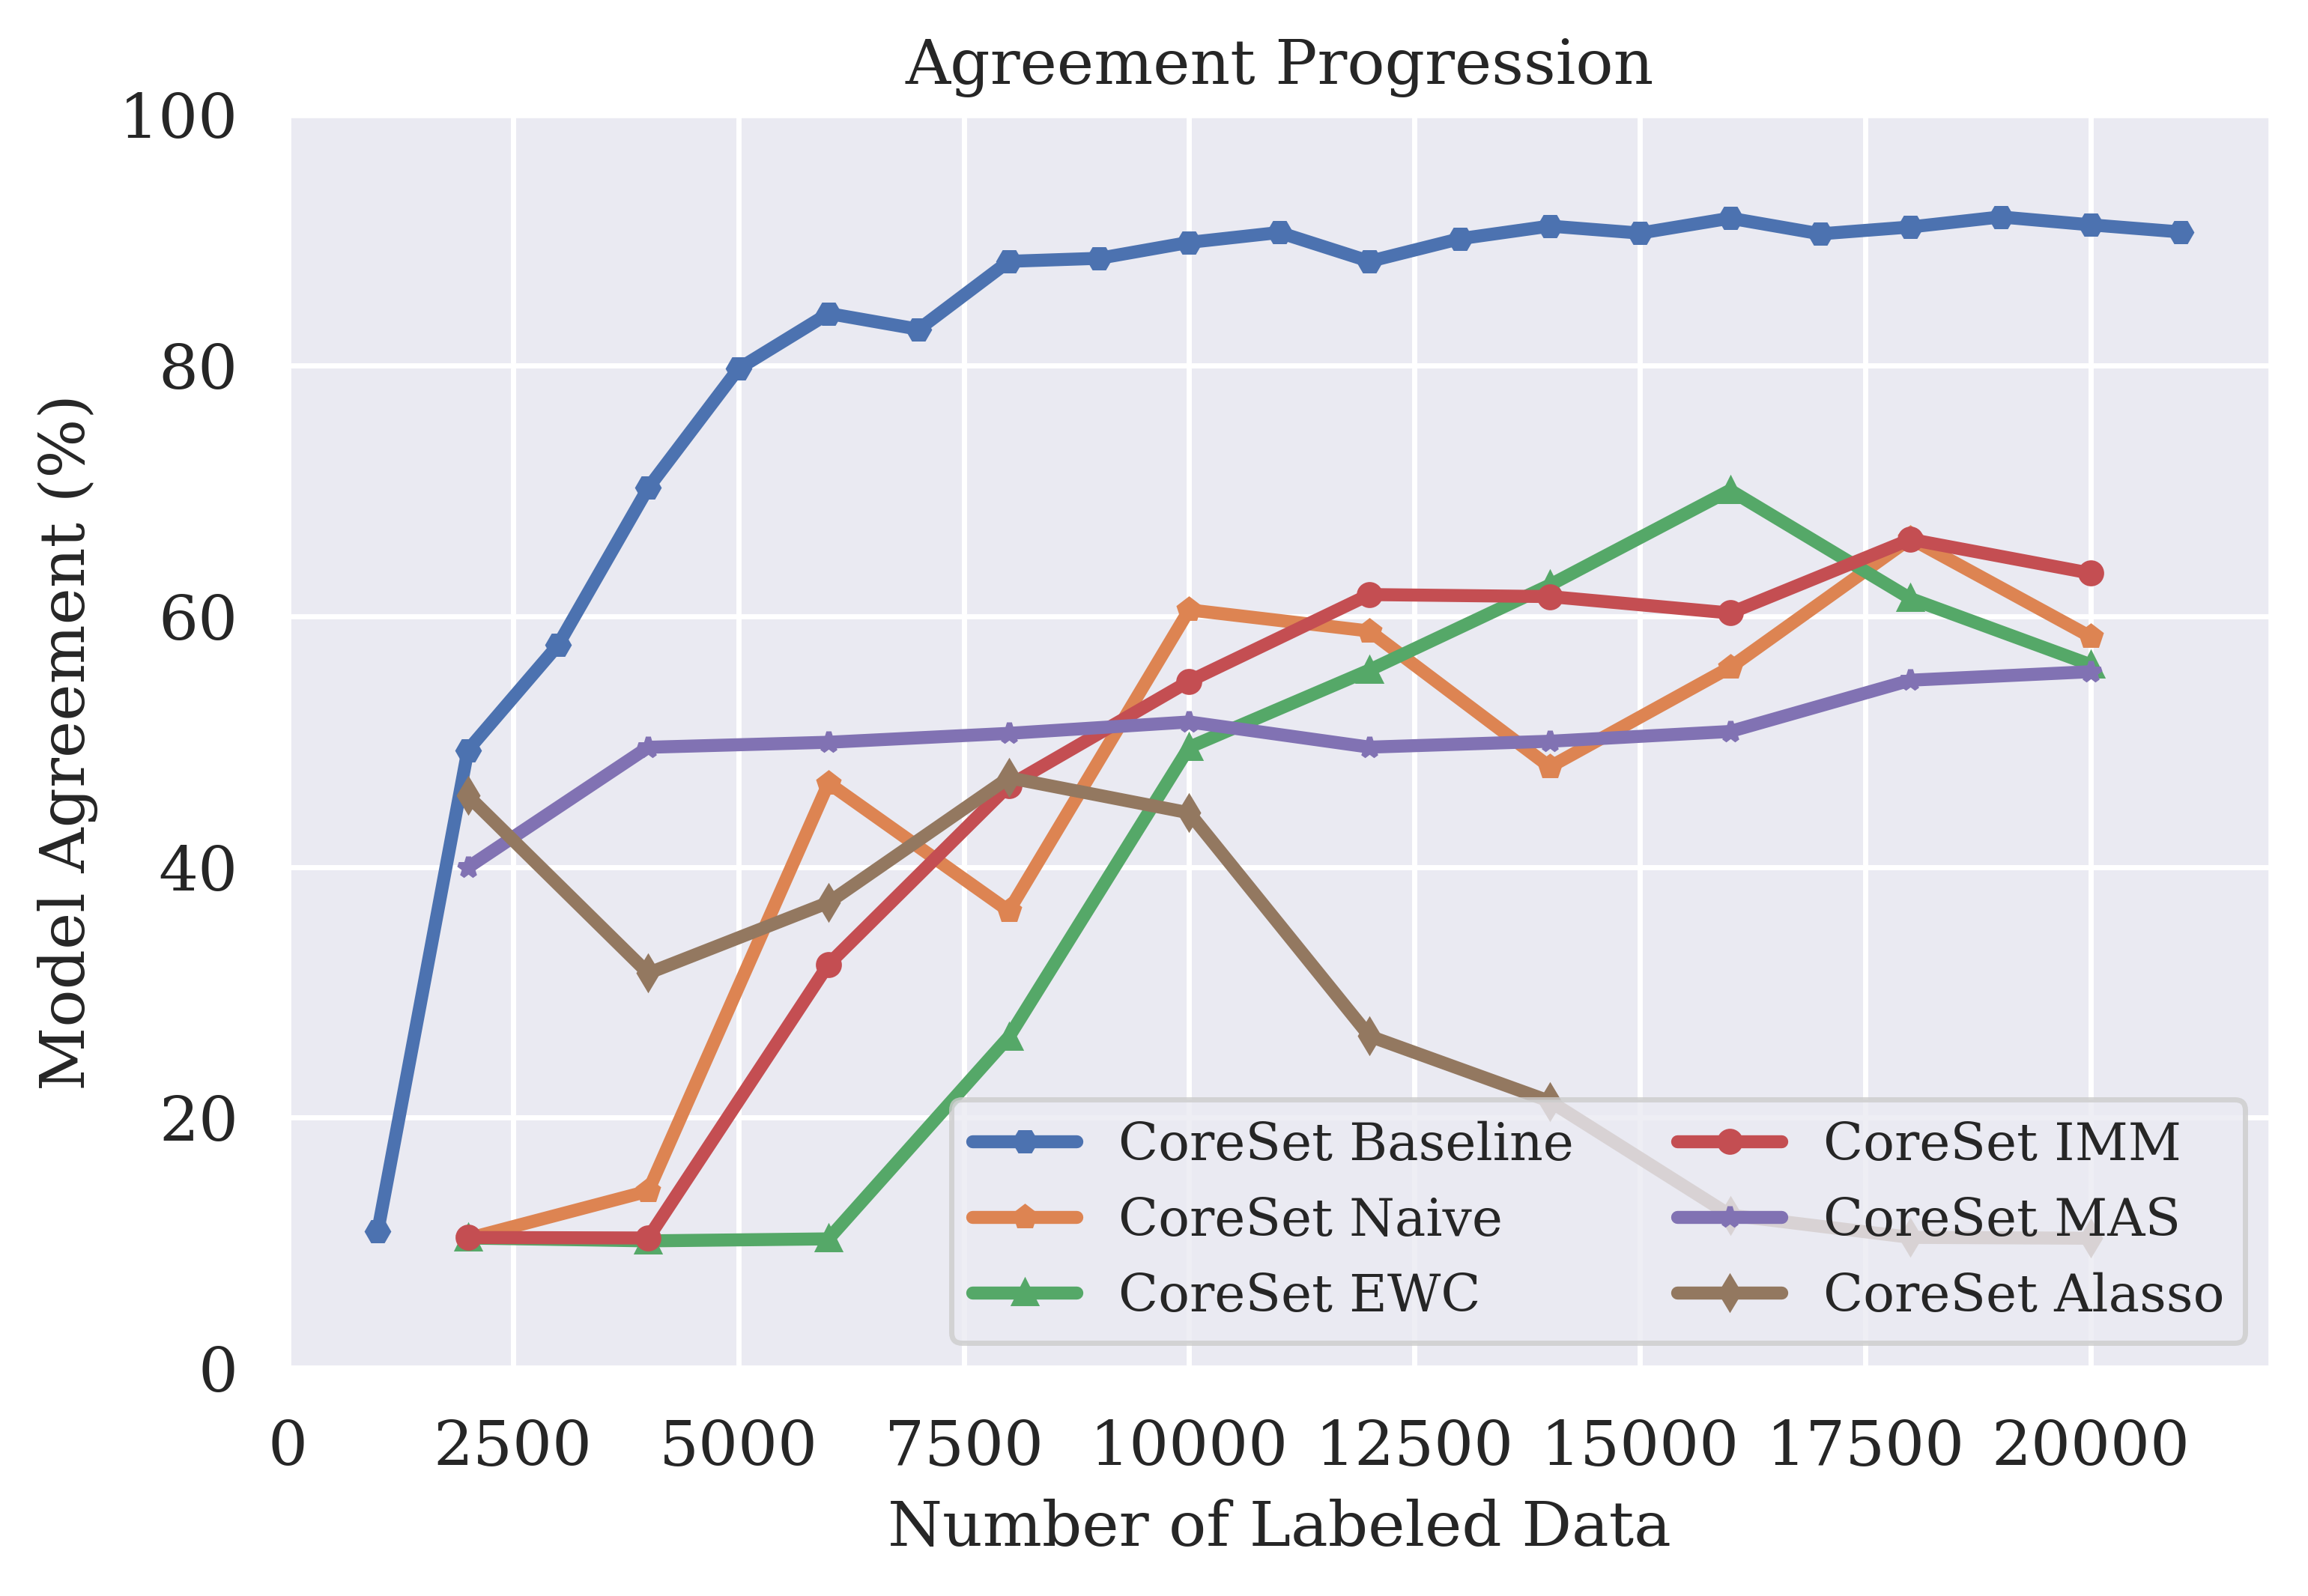
\includegraphics[width=0.7\linewidth]{images/results_CALMS/mnist_softmax_coreset.png}
    \caption[Agreement Comparison for Model Stealing on MNIST using the softmax output and the Active Learning strategy CoreSet]{Progression of Model Agreement
    (in \%) for Model Stealing Attacks using Continual Active Learning on the MNIST dataset. We use Model Stealing Attacks with the Active Learning strategy
    CoreSet and train using the softmax output of the Target Model.}
    \label{fig:CALMSMNISTSoftmaxCoreSet}
\end{figure}

\begin{figure}[h]
    \centering
    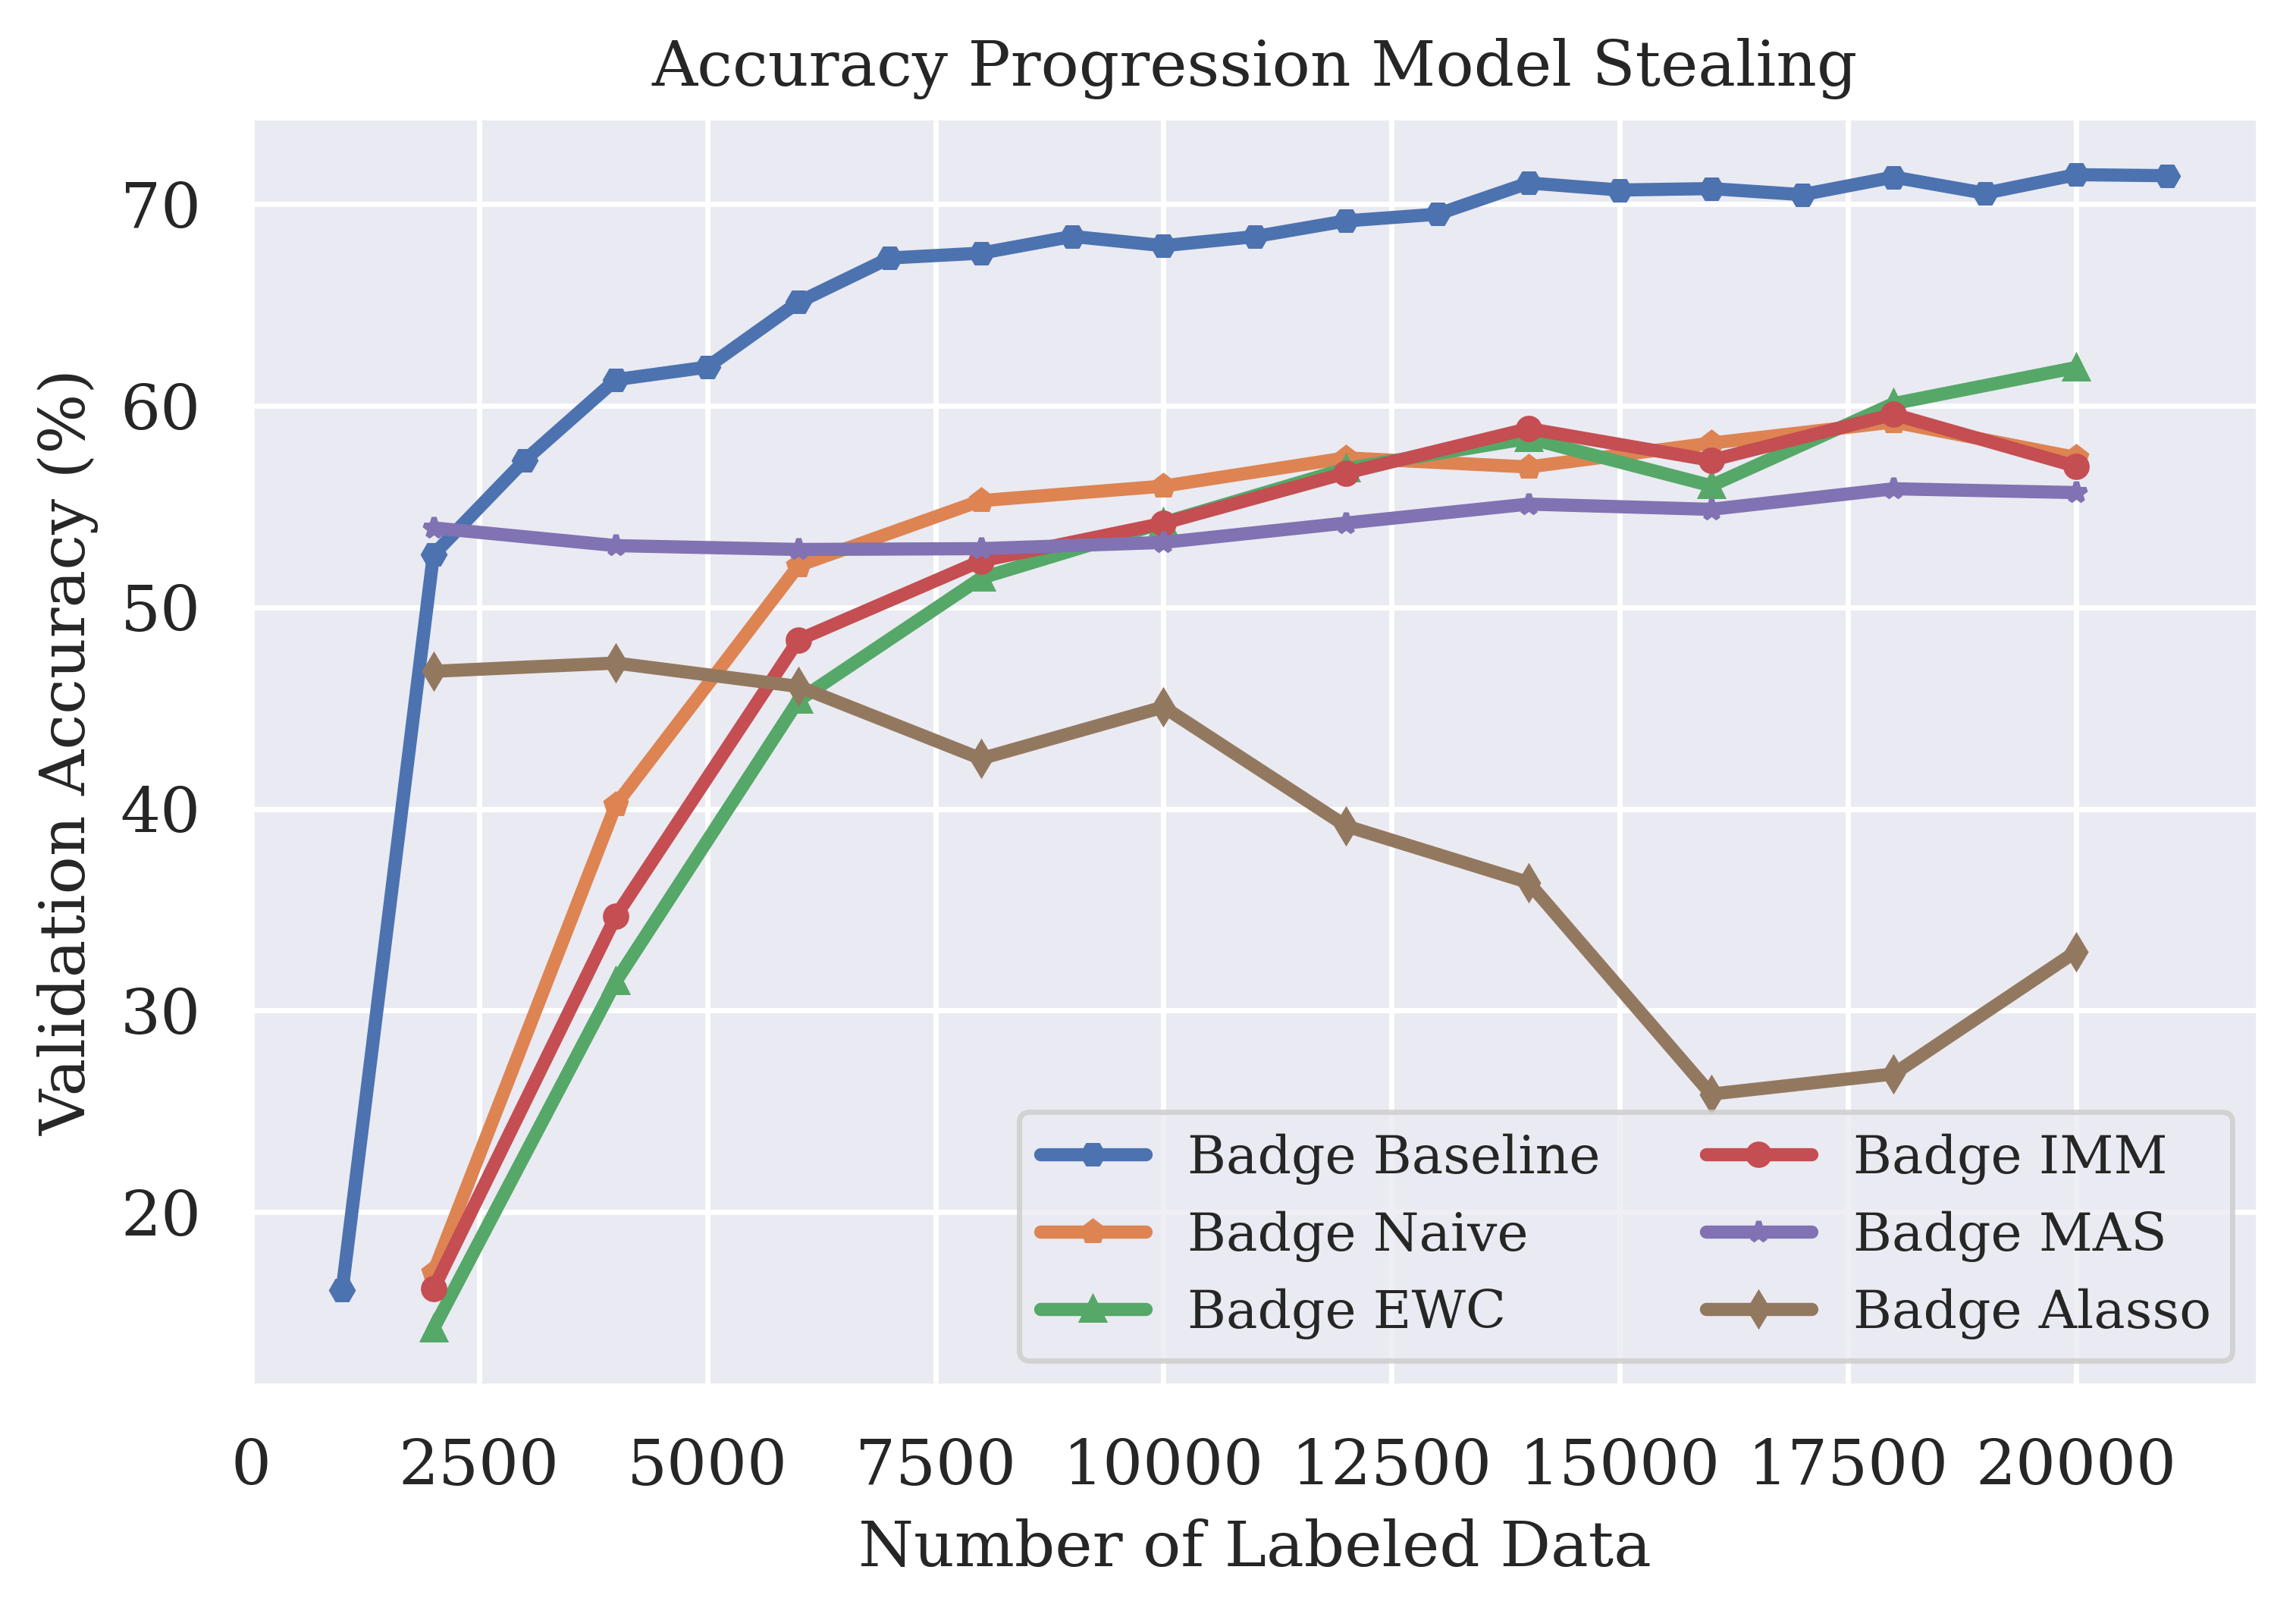
\includegraphics[width=0.7\linewidth]{images/results_CALMS/cifar_softmax_badge.png}
    \caption[Agreement Comparison for Model Stealing on MNIST using the softmax output and the Active Learning strategy Badge]{Progression of Model Agreement
    (in \%) for Model Stealing Attacks using Continual Active Learning on the MNIST dataset. We use Model Stealing Attacks with the Active Learning strategy
    \gls{badge} and train using the softmax output of the Target Model.}
    \label{fig:CALMSMNISTSoftmaxBadge}
\end{figure}

%VAAL AGEM
\begin{figure}[h]
    \centering
    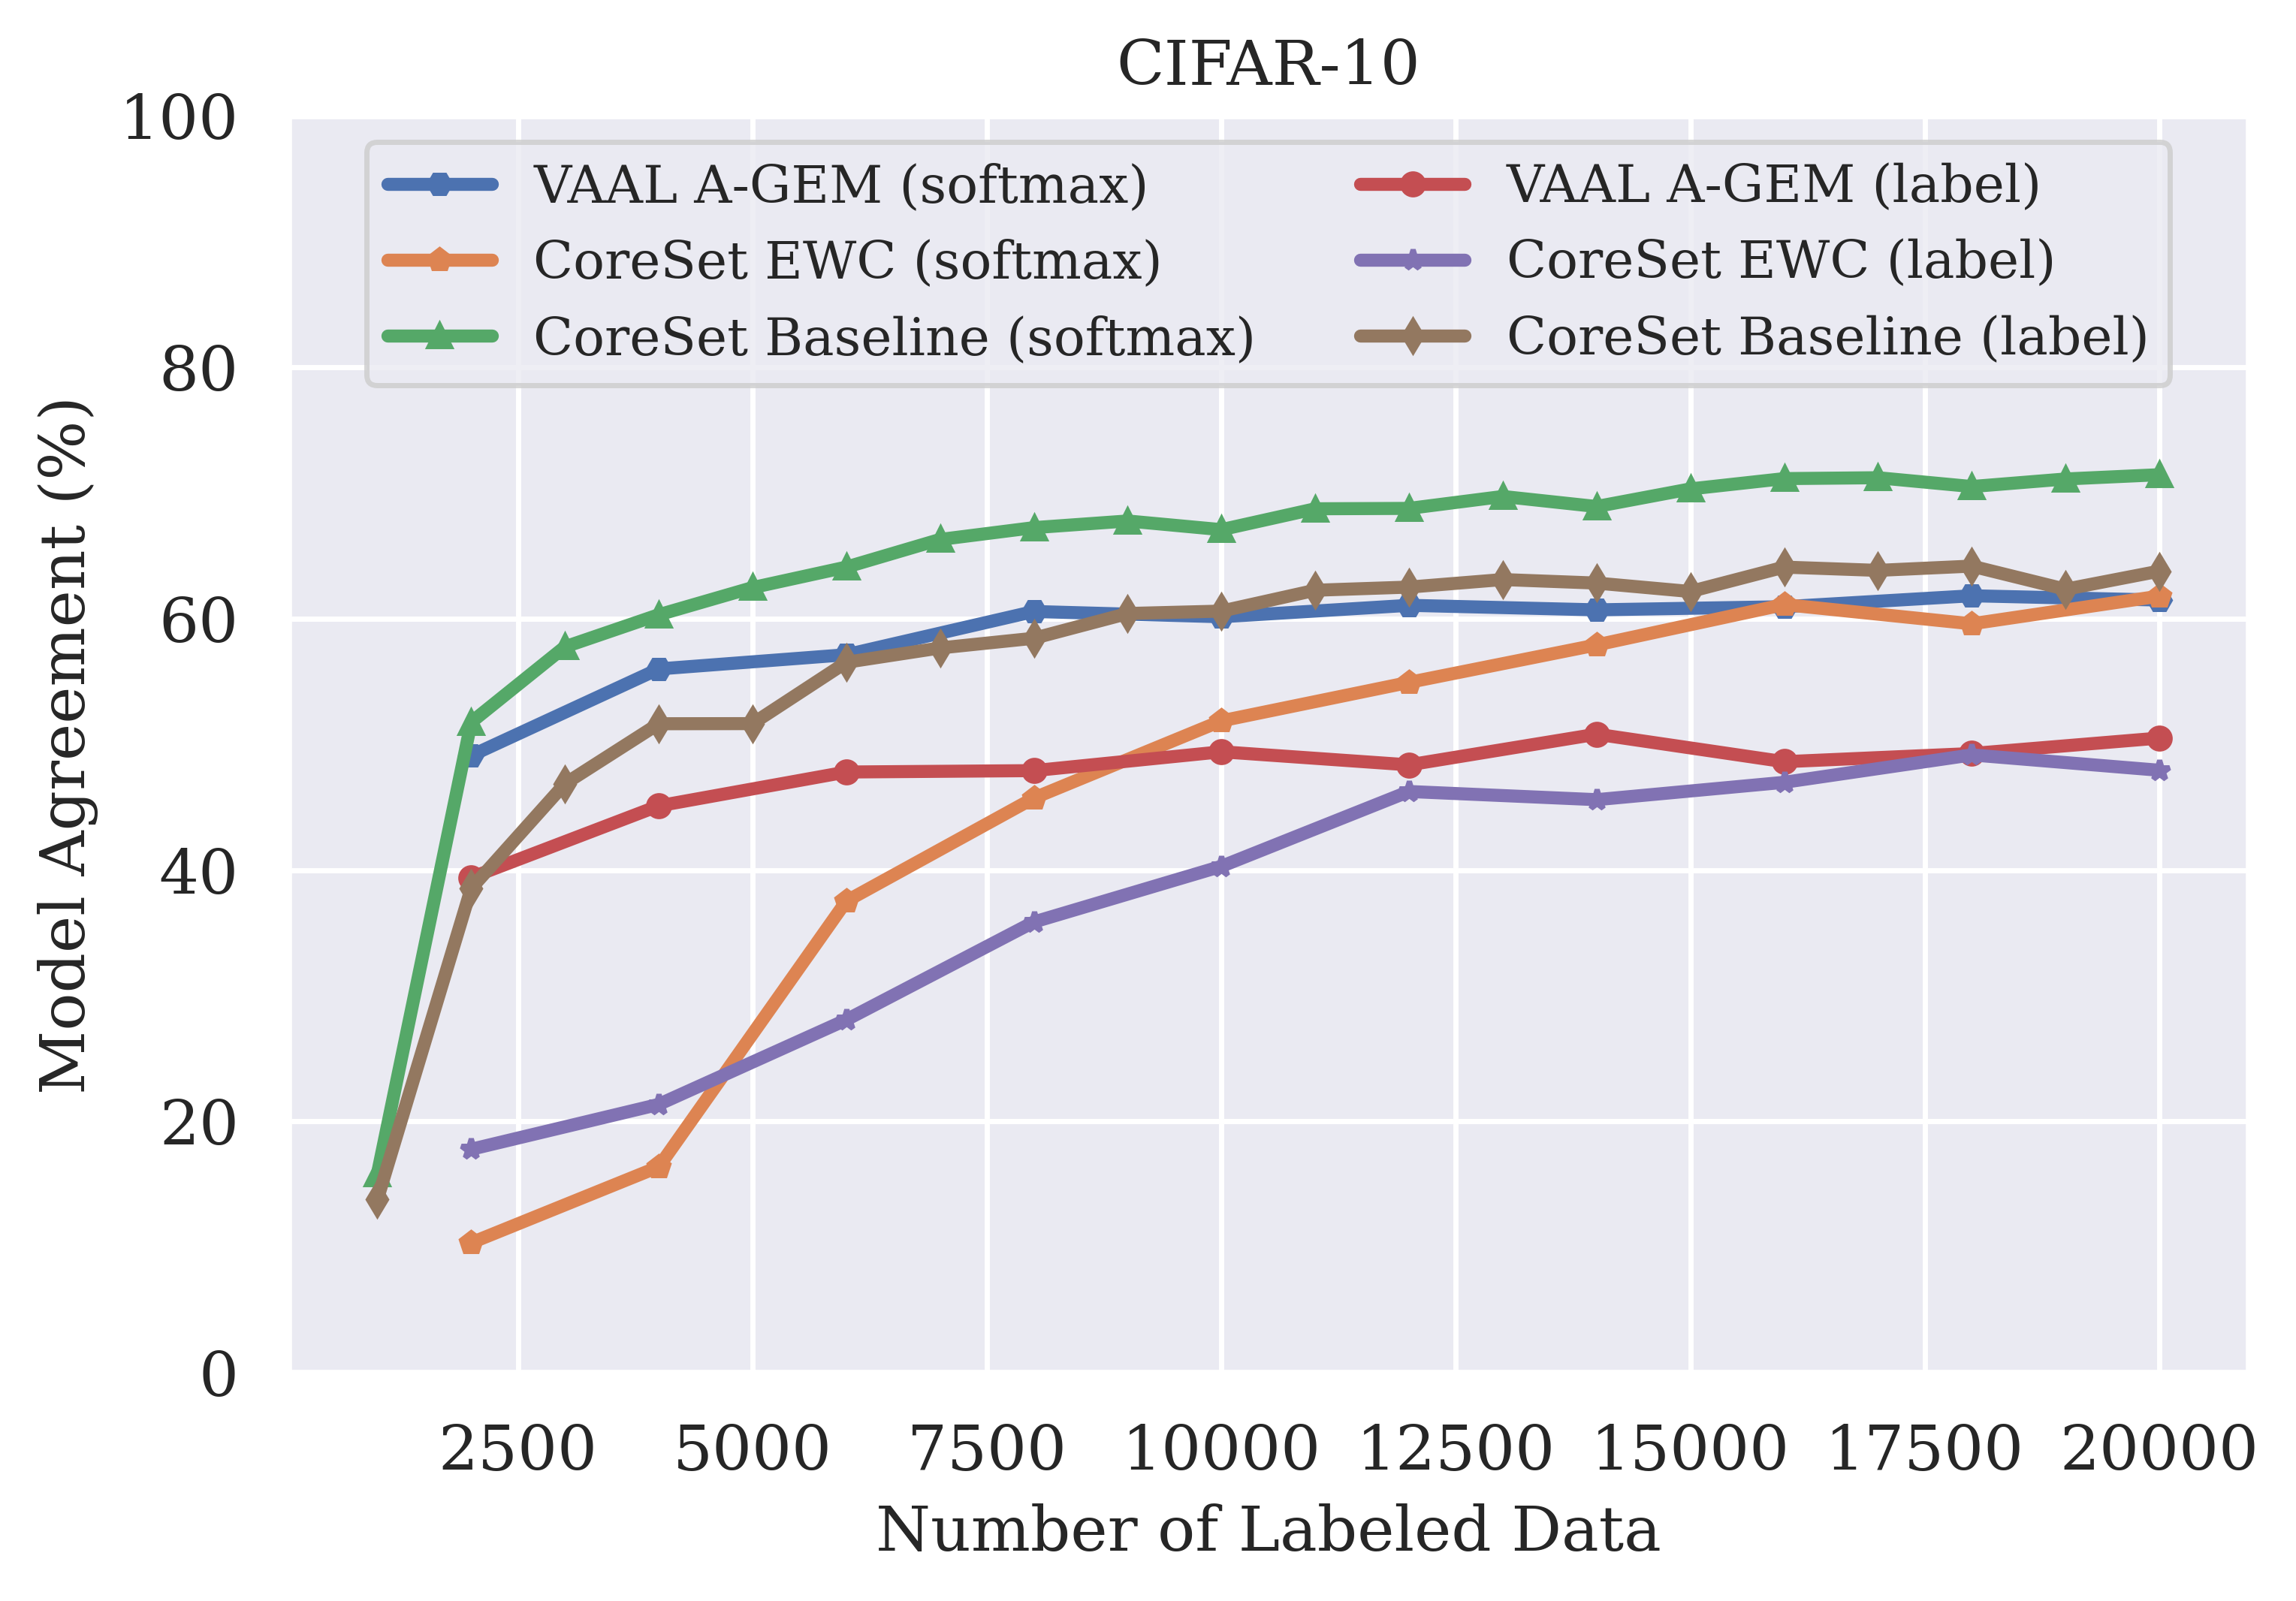
\includegraphics[width=0.7\linewidth]{images/results_CALMS/cifar_vaal_agem.png}
    \caption[Agreement Comparison for Model Stealing on CIFAR-10 using VAAL and AGEM]{Progression of Model Agreement (in \%)
    for Continual Active Learning using \gls{vaal} and \gls{a-gem}, CoreSet and \gls{ewc} as well as the CoreSet Baseline.
    We use a total budget of 20000 samples and CIFAR-10 as our Target Model Dataset}
    \label{fig:CALMScifarVAAL_AGEM}
\end{figure}

\begin{figure}[h]
    \centering
    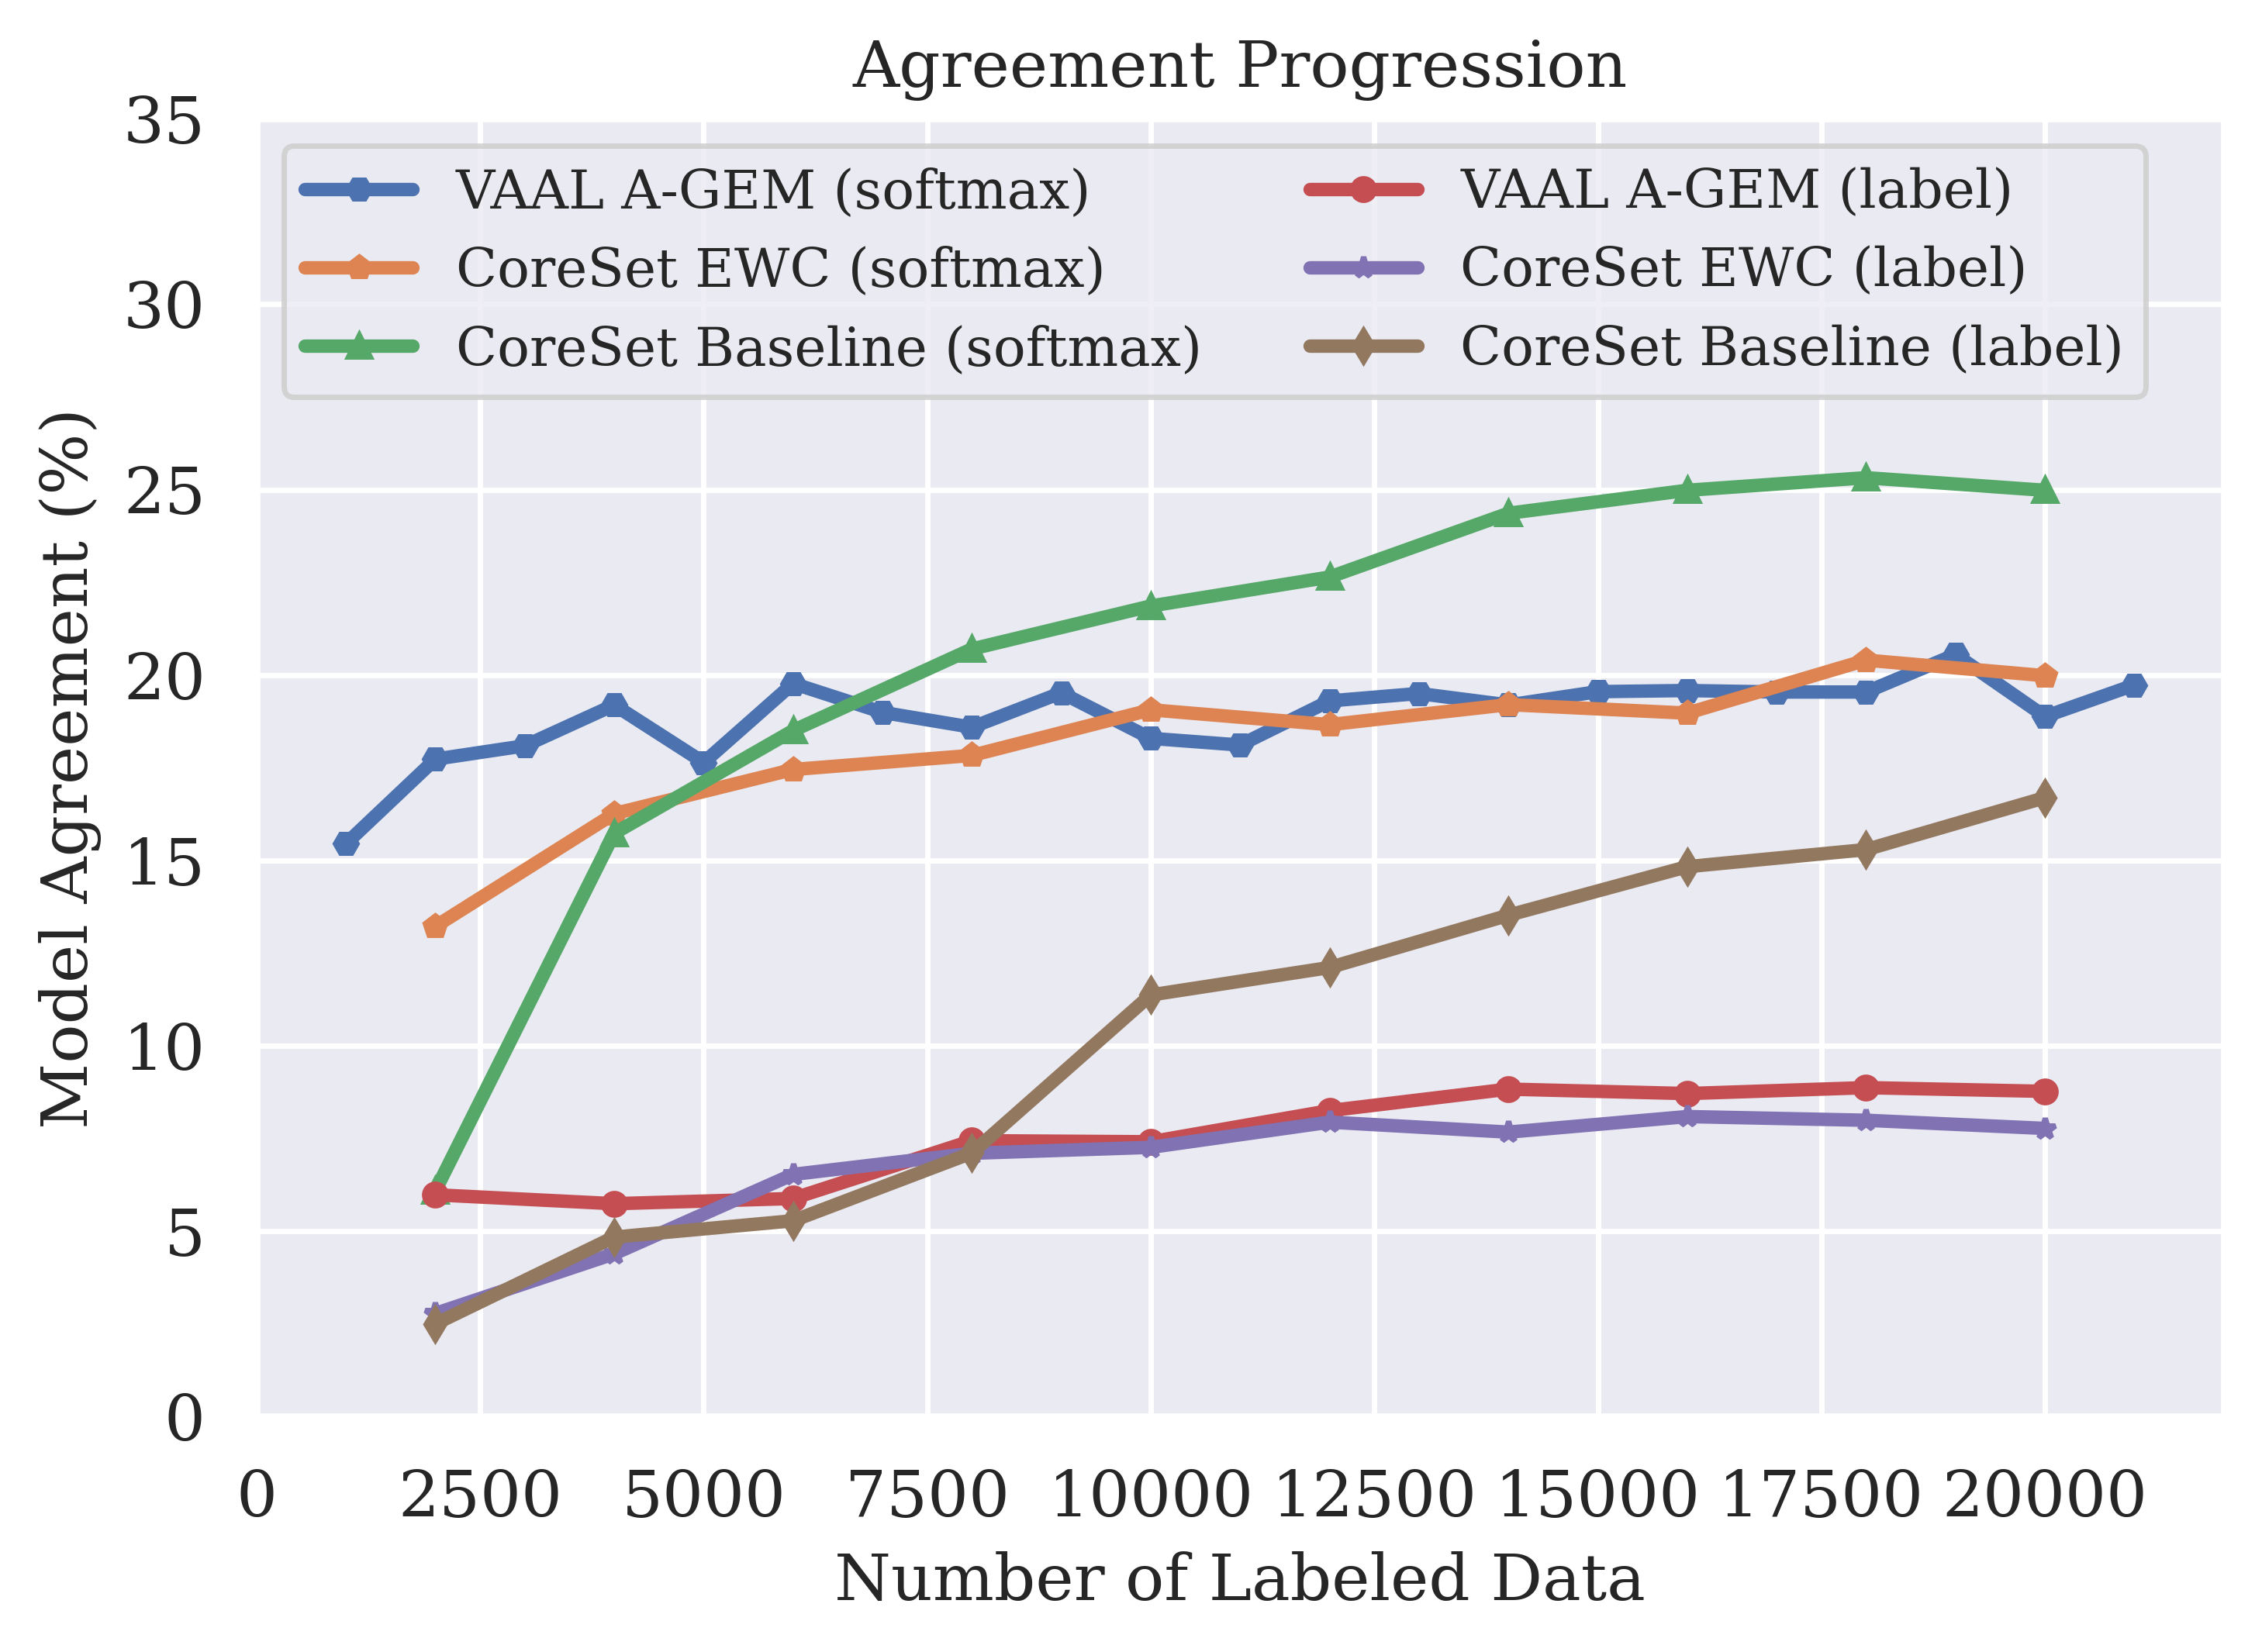
\includegraphics[width=0.7\linewidth]{images/results_CALMS/cifar100_vaal_agem.png}
    \caption[Agreement Comparison for Model Stealing on CIFAR-100 using VAAL and AGEM]{Progression of Model Agreement (in \%)
    for Continual Active Learning using \gls{vaal} and \gls{a-gem}, CoreSet and \gls{ewc} as well as the CoreSet Baseline.
    We use a total budget of 20000 samples and CIFAR-100 as our Target Model Dataset}
    \label{fig:CALMScifar100VAAL_AGEM}
\end{figure}

\begin{figure}[h]
    \centering
    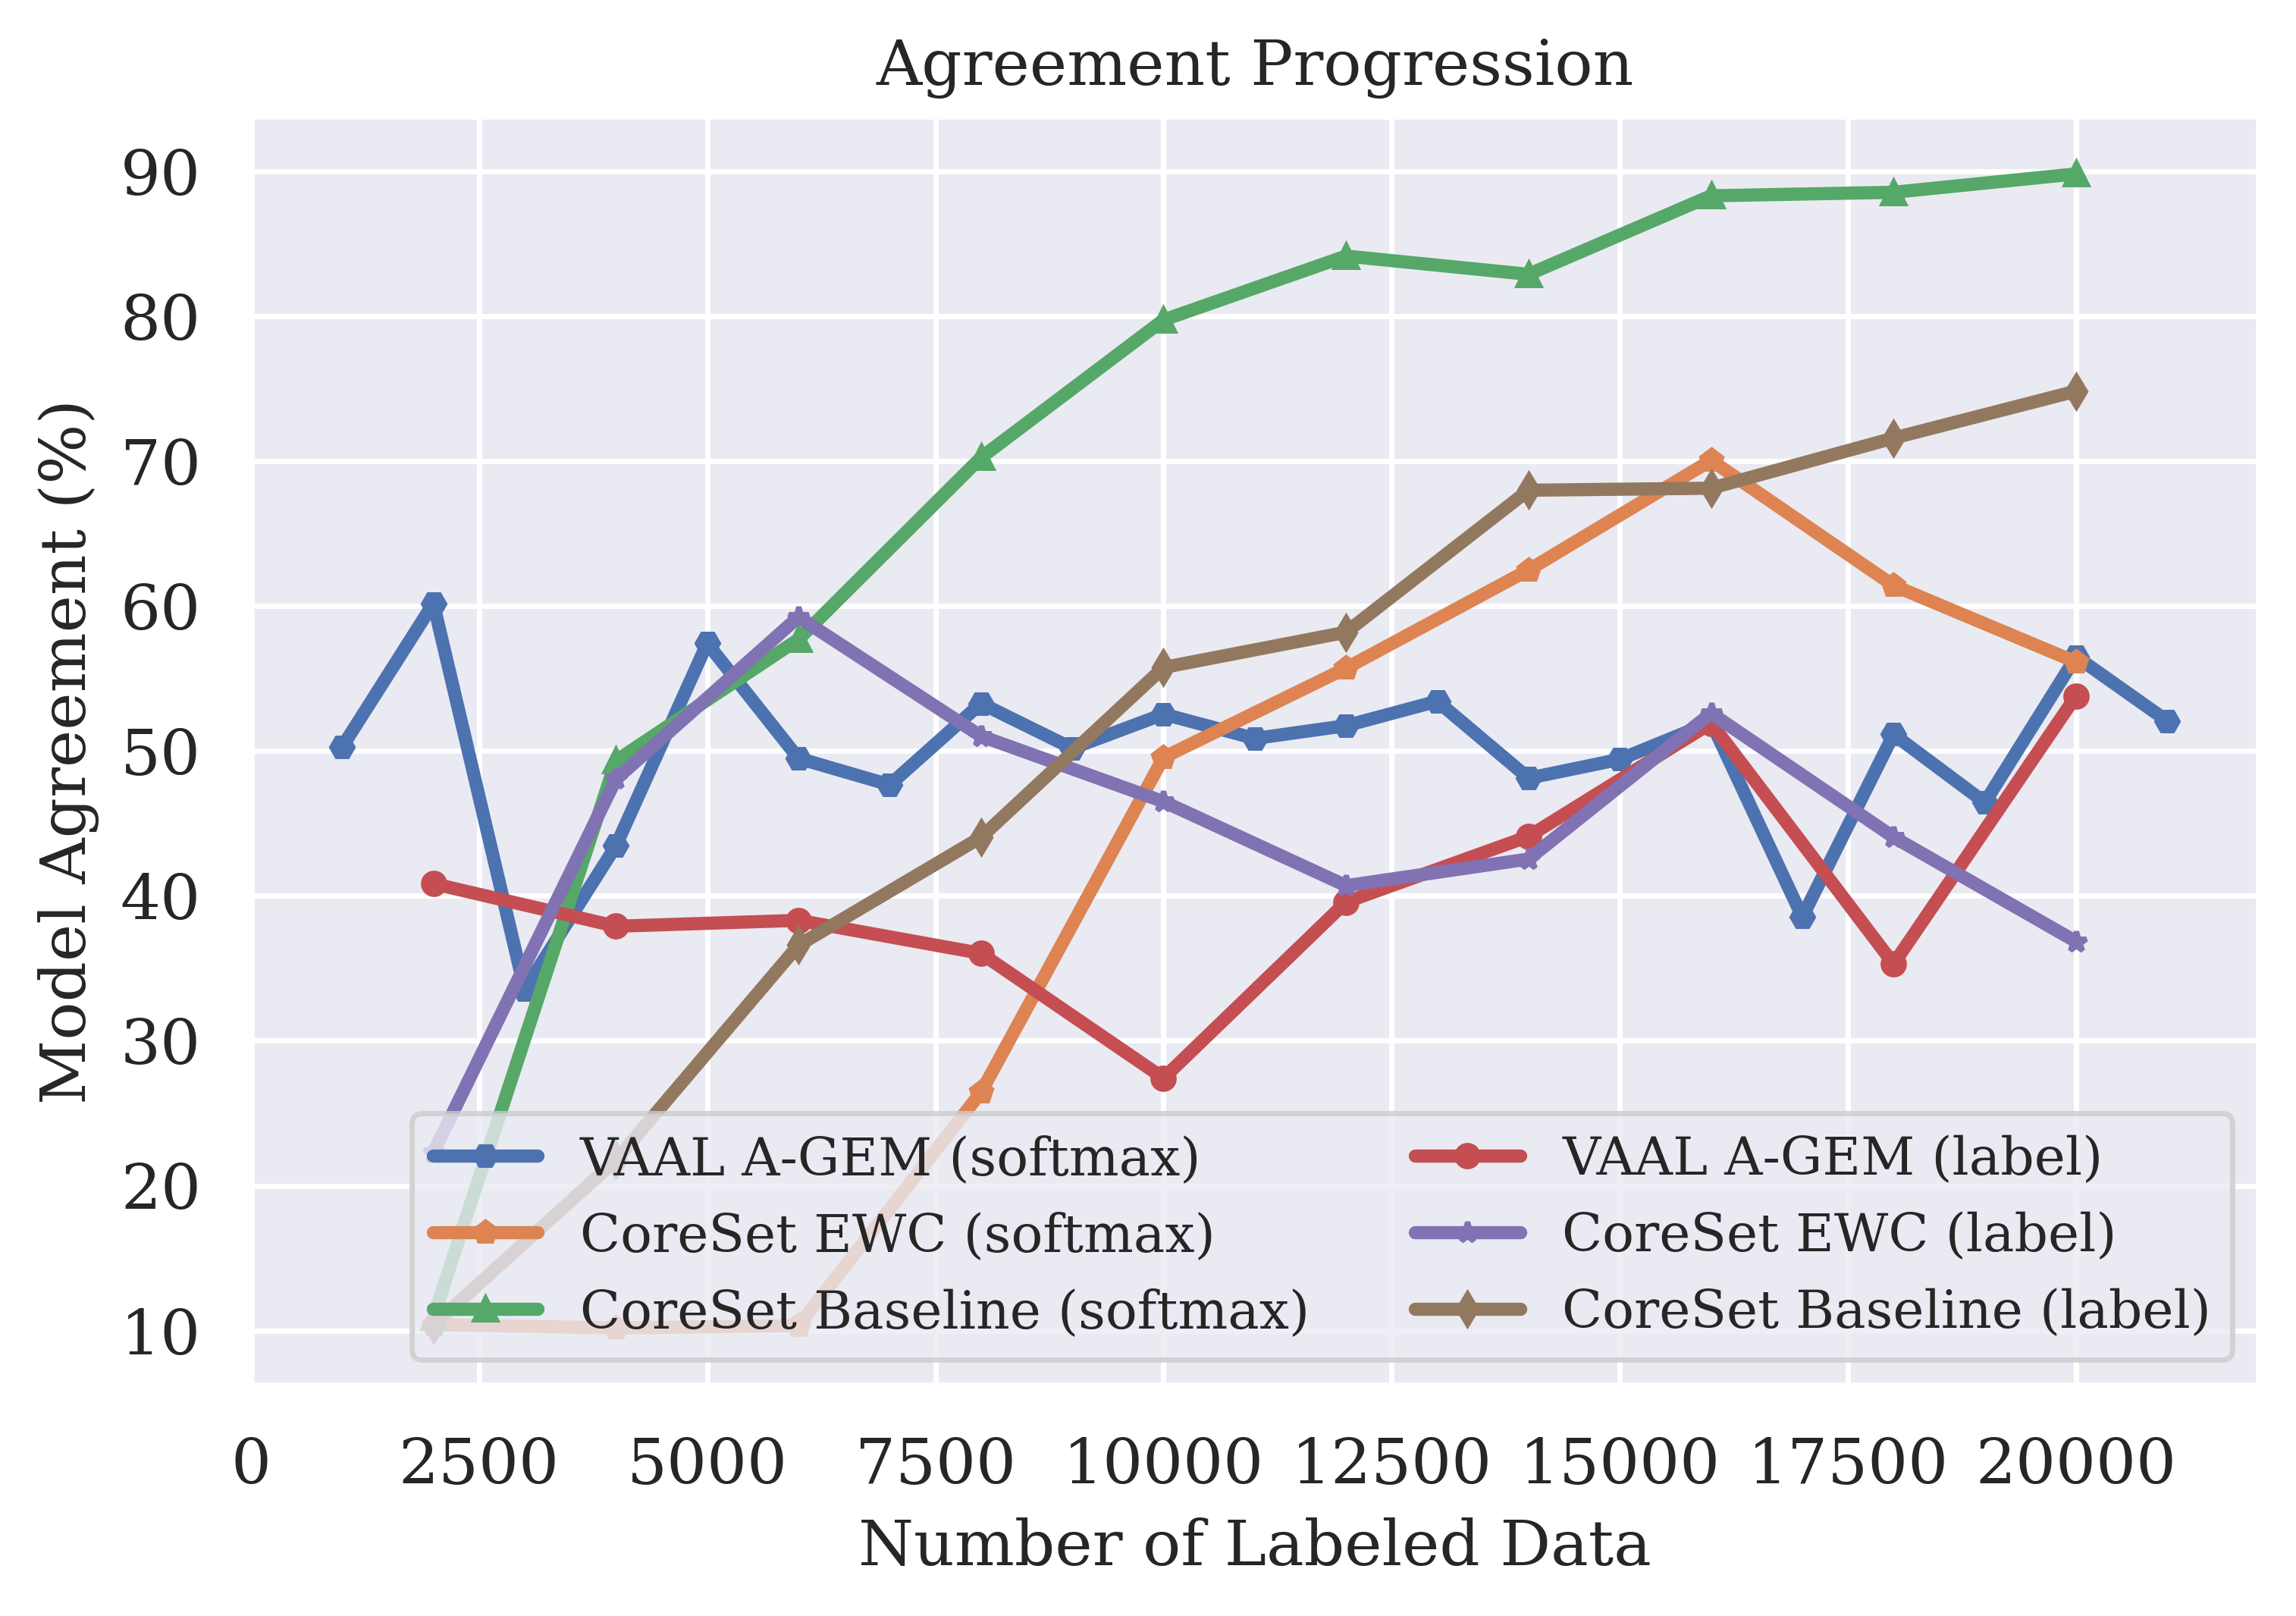
\includegraphics[width=0.7\linewidth]{images/results_CALMS/mnist_vaal_agem.png}
    \caption[Agreement Comparison for Model Stealing on MNIST using VAAL and AGEM]{Progression of Model Agreement (in \%)
    for Continual Active Learning using \gls{vaal} and \gls{a-gem}, CoreSet and \gls{ewc} as well as the CoreSet Baseline.
    We use a total budget of 20000 samples and MNIST as our Target Model Dataset}
    \label{fig:CALMSmnistVAAL_AGEM}
\end{figure}